% abnTeX2: Modelo de Trabalho Academico (tese de doutorado, dissertacao de
% mestrado e trabalhos monograficos em geral) em conformidade com 
% ABNT NBR 14724:2011: Informacao e documentacao - Trabalhos academicos - Apresentação
% Disponível em: https://github.com/abntex/abntex2/blob/master/doc/latex/abntex2/examples/abntex2-modelo-trabalho-academico.tex

% Configurações do documento:
\documentclass[12pt, openright, twoside, a4paper, english, french, spanish, brazil]{abntex2}
% \documentclass[12pt, openright, twoside, a4paper, english, french, spanish, brazil]{abntex2}

% Pacotes básicos:
\usepackage{lmodern}
\usepackage[T1]{fontenc}
\usepackage[utf8]{inputenc}
\usepackage{indentfirst}
\usepackage{color}
\usepackage{graphicx}
% Adicionados (ou com opções adicionadas) por Bruno:
\usepackage[nopatch=all]{microtype}
\usepackage[most]{tcolorbox}
\usepackage{listingsutf8}
\usepackage{enumerate}

% Pacotes adicionais, usados apenas no âmbito do Modelo Canônico do abnteX2:
\usepackage{lipsum}

% Pacotes de citações:
\usepackage[brazilian,hyperpageref]{backref}
\usepackage[alf]{abntex2cite}

% Configurações do pacote backref:
\renewcommand{\backrefpagesname}{Citado na(s) página(s):~}
\renewcommand{\backref}{}
\renewcommand*{\backrefalt}[4]{
	\ifcase #1 
		Nenhuma citação no texto.
	\or
		Citado na página #2.
	\else
		Citado #1 vezes nas páginas #2.
	\fi
}

% Capa e Folha de Rosto:
% Informações para CAPA e FOLHA DE ROSTO:
\titulo{Formalização do Símbolo de Legendre em \textit{Coq}}
\autor{Bruno Rafael dos Santos}
\local{Brasil}
\data{\today}
\orientador{Karina Girardi Roggia}
\coorientador{Paulo Henrique Torrens}
\instituicao{
  Universidade do Estado de Santa Catarina -- UDESC
  % \par
  % Departamento de Ciência da Computação
  \par
  Bacharelado em Ciência da Computação
}

\tipotrabalho{Trabalho de Conclusão de Curso}
% O preambulo deve conter o tipo do trabalho, o objetivo, 
% o nome da instituição e a área de concentração 
\preambulo{Trabalho de Conclusão de Curso apresentado ao curso de Bacharelado em Ciência da Computação do Centro de Ciências Tecnológicas da Universidade do Estado de Santa Catarina, como requisito parcial para a obtenção do grau de Bacharel em Ciência da Computação.}

% \preambulo{Trabalho de Conclusão de Curso apresentado como requisito parcial para obtenção do título de Bacharelado em Ciência da Computação pelo Centro de Ciências Tecnológicas da Universidade do Estado de Santa Catarina, como requisito parcial para a obtenção do grau de Bacharel em Ciência da Computação.}
% Outras configurações:
% ---- Arquivo com as configurações do PDF

% Alteração para fonte de capítulos:
\renewcommand{\ABNTEXchapterfont}{\normalfont}
\renewcommand{\ABNTEXchapterfont}{\bfseries}

% Definindo a cor azul em RGB:
\definecolor{blue}{RGB}{41,5,195}

% Informações do PDF:
\makeatletter
\hypersetup{
		pdftitle={\@title}, 
		pdfauthor={\@author},
    	pdfsubject={\imprimirpreambulo},
	    pdfcreator={Bruno Rafael dos Santos},
		pdfkeywords={Algoritmo \textit{RESSOL}}{Algoritmo de Tonelli-Shanks}{Lei de Reciprocidade Quadrática}{abntex2}{trabalho acadêmico}, 
		colorlinks=true,
    	linkcolor=blue,
    	citecolor=blue,
    	filecolor=magenta,
		urlcolor=blue,
		bookmarksdepth=4
}
\makeatother

% Posiciona figuras e tabelas no topo da página quando adicionadas sozinhas em uma página em branco (ver https://github.com/abntex/abntex2/issues/170):
\makeatletter
\setlength{\@fptop}{5pt} 
\makeatother

% Possibilita criação de Quadros e Lista de quadros (ver https://github.com/abntex/abntex2/issues/176):
\newcommand{\quadroname}{Quadro}
\newcommand{\listofquadrosname}{Lista de quadros}
\newfloat[chapter]{quadro}{loq}{\quadroname}
\newlistof{listofquadros}{loq}{\listofquadrosname}
\newlistentry{quadro}{loq}{0}

% Configurações para atender às regras da ABNT
\setfloatadjustment{quadro}{\centering}
\counterwithout{quadro}{chapter}
\renewcommand{\cftquadroname}{\quadroname\space} 
\renewcommand*{\cftquadroaftersnum}{\hfill--\hfill}

\setfloatlocations{quadro}{hbtp} % Ver https://github.com/abntex/abntex2/issues/176

% O tamanho do parágrafo é dado por:
\setlength{\parindent}{1.3cm}

% Controle do espaçamento entre um parágrafo e outro:
\setlength{\parskip}{0.2cm}  % tente também \onelineskip

% Configurações adicionadas por Bruno:
	% % Do .tex da UDESC:
	% 	% Comando para inverter sobrenome e nome
	% 	\newcommand{\invertname}[1]{%
	% 	\StrBehind{#1}{{}}, \StrBefore{#1}{{}}%
	% 	}%  
	% Teoremas e etc:
		\newtheorem{definição}{Definição}
		\newtheorem{teorema}{Teorema}
		\newtheorem{lema}{Lema}
	% Operadores e etc:
		\usepackage{amsmath, amsfonts, amssymb}
		\usepackage{mathtools}
		\DeclareMathOperator{\mdc}{mdc}
		\DeclareMathOperator{\mmc}{mmc}
		\DeclarePairedDelimiter\abs{\lvert}{\rvert}
		\usepackage{proof}
		\usepackage{mathpartir}
		\newcommand{\qed}{\hfill $\blacksquare$}
	% Highlight de código em coq:
		\definecolor{violet}{RGB}{80,5,100}
		\definecolor{teal}{RGB}{0,128,128}
		\definecolor{orange}{RGB}{255,128,13}
		\definecolor{darkgreen}{RGB}{0,100,0}
		\definecolor{darkred}{RGB}{100,0,0}
		\definecolor{dkpink}{RGB}{231,84,128}
		\usepackage{listings, Estilos/coq, Estilos/coq-error}
	% Algoritmos:
		\usepackage[portuguese,linesnumbered,boxruled,noend]{algorithm2e}
		\usepackage{hyperref}
		\SetArgSty{textnormal}
		\SetNlSty{textbf}{}{:}
		\setlength{\algomargin}{2.5em}
		\SetKwInput{Entrada}{Entrada}
		\SetKwInput{Saida}{Sa\'{i}da}
		\SetKw{Retorna}{retorna}
		\SetKwFor{Enqto}{enquanto}{faça}{endw}
		\SetKwIF{Se}{eSe}{SeN}{se}{então}{e se}{senão}{fimse}
		% Comandos para suprimir e reativar numeração em lstlisting:
		\let\origthelstnumber\thelstnumber
		\makeatletter
		\newcommand*\Suppressnumber{%
		\lst@AddToHook{OnNewLine}{%
			\let\thelstnumber\relax%
			\advance\c@lstnumber-\@ne\relax%
			}%
		}

		\newcommand*\Reactivatenumber{%
		\lst@AddToHook{OnNewLine}{%
		\let\thelstnumber\origthelstnumber%
		\advance\c@lstnumber\@ne\relax}%
		}
		\makeatother
		% Comando para \vdots customizado:
		\makeatletter
		\DeclareRobustCommand{\rvdots}{%
		\vbox{
			\baselineskip4\p@\lineskiplimit\z@
			\kern-\p@
			\hbox{.}\hbox{.}\hbox{.}
		}}
		\makeatother

% Compilar índice:
\makeindex

% Início do documento:
\begin{document}
\selectlanguage{brazil}
\frenchspacing 
	% Elementos pré-textuais:
	\pretextual
	% Capa:
	\imprimircapa
	% Folha de rosto (o '*' indica que haverá a ficha bibliográfica):
	\imprimirfolhaderosto*{}
	% Ficha Catalográfica:
	% \begin{fichacatalografica}
% 	\sffamily
% 	\vspace*{\fill}					% Posição vertical
% 	\begin{center}					% Minipage Centralizado
% 	\fbox{
%         \begin{minipage}[c][7cm]{12.5cm}		% Largura
%         % \begin{minipage}[c][8cm]{13.5cm}		% Largura
%         \small
%         \imprimirautor
%         %Sobrenome, Nome do autor
        
%         \hspace{0.5cm} \imprimirtitulo  / \imprimirautor. --
%         \imprimirlocal, \imprimirdata-
        
%         \hspace{0.5cm} \thelastpage p. : il. (algumas color.) ; 30 cm.\\
        
%         % \hspace{0.5cm} \imprimirorientadorRotulo~\imprimirorientador\\
%         % Editado por Bruno (parte de orientador e coorientador):
%         \hspace{0.5cm} \imprimirorientadorRotulo~\imprimirorientador
%         \par \hspace{0.5cm} \imprimircoorientadorRotulo~\imprimircoorientador \\
        
%         \hspace{0.5cm}
%         \parbox[t]{\textwidth}{\imprimirtipotrabalho~--~\\\imprimirinstituicao,
%         \imprimirdata.}\\
        
%         \hspace{0.5cm}
%             1. símbolo de Legendre.
%             2. criptografia.
%             3. Teoria dos Números.
%             I. Karina Girardi Roggia.
%             II. Universidade do Estado de Santa Catarina.
%             III. Faculdade de Ciência da Computação.
%             IV. Formalização do \textit{Símbolo de Legendre} em \textit{Coq}. 			
%         \end{minipage}
%     }
% 	\end{center}
% \end{fichacatalografica}

% Código de ficha catalográfica do .tex da UDESC:

\begin{fichacatalografica}
	%\sffamily
	%\rmfamily
	\ttfamily \hbadness=10000
	\vspace*{\fill}					% Posição vertical
	\begin{center}					% Minipage Centralizado
	% Para gerar a ficha catalográfica de teses e \\ 
	% dissertações acessar o link:  \\
	% https://www.udesc.br/bu/manuais/ficha
	
	\vspace*{8pt}
	
%	\begin{minipage}[c]{8cm}
%	\centering \sffamily
%	 Ficha catalográfica elaborada pelo(a) autor(a), com auxílio do programa de geração automática da Biblioteca Setorial do CCT/UDESC
%	\end{minipage}
	\fbox{
        \begin{minipage}[c]{12.5cm}		% Largura
	        \flushright
            {
                \begin{minipage}[c]{10.5cm}		% Largura
                \vspace{1.25cm}
                %\footnotesize
                \setlength{\parindent}{1.5em}
                % \noindent \invertname{\imprimirautor} \par
                \noindent dos Santos, Bruno Rafael \par
                \imprimirtitulo{ }/{ }\imprimirautor. -- \imprimirlocal, \imprimirdata .\par
                \pageref{LastPage} p. : il. ; 30 cm.\par
                \vspace{1.5em}
                \imprimirorientadorRotulo~\imprimirorientador.\par
                \imprimircoorientadorRotulo~\imprimircoorientador.\par
                \imprimirtipotrabalho~--~\imprimirinstituicao, \imprimirlocal, \imprimirdata.\par
                \vspace{1.5em}
                    1. símbolo de Legendre.
                    2. criptografia.
                    3. Teoria dos Números.
                    % 4. Palavra-chave.
                    % 5. Palavra-chave.
                    % I. \invertname{\imprimirorientador}.
                    I. Roggia, Karina Girardi.
                    % II. \invertname{\imprimircoorientador}.
                    II. Torrens, Paulo Henrique.
                    III. \imprimirinstituicao.
                    % IV. Título. %
                    IV. Formalização do \textit{Símbolo de Legendre} em \textit{Coq}. %
                \vspace{1.25cm}	%		
                \end{minipage}%
            }% 
	    \end{minipage}
    }%
	\vspace*{0.5cm}
	\end{center}
\end{fichacatalografica}

	% \begin{errata}
	% 	Elemento opcional.
	% \end{errata}

	\begin{folhadeaprovacao}
	\begin{center}
	  {\ABNTEXchapterfont\large\imprimirautor}
	  \vspace*{\fill}\vspace*{\fill}
	  \begin{center}
		\ABNTEXchapterfont\bfseries\Large\imprimirtitulo
	  \end{center}
	  \vspace*{\fill}
	  \hspace{.45\textwidth}
	  \begin{minipage}{.5\textwidth}
		  \imprimirpreambulo
	  \end{minipage}%
	  \vspace*{\fill}
	 \end{center}
		  
	 Trabalho aprovado. \imprimirlocal, 24 de novembro de 2012:
  
	 \assinatura{\textbf{\imprimirorientador} \\ Orientadora (Doutora)} 
	 \assinatura{\textbf{Cristiano Damiani Vasconcelos} \\ Doutor}
	 \assinatura{\textbf{Rafael Castro Gonçalves} \\ Mestre}
	 \assinatura{\textbf{Paulo Henrique Torrens} \\ Co-orientador}
		
	 \begin{center}
	  \vspace*{0.5cm}
	  {\large\imprimirlocal}
	  \par
	  {\large\imprimirdata}
	  \vspace*{1cm}
	\end{center}
	
\end{folhadeaprovacao}

% \begin{dedicatoria}
% 	\vspace*{\fill}
% 	\centering
% 	\noindent
% 	\textit{ Este trabalho é dedicado às crianças adultas que,\\
% 	quando pequenas, sonharam em se tornar cientistas.} \vspace*{\fill}
% \end{dedicatoria}

\begin{agradecimentos}
	Incialmente agradeço a Laurent Théry pelas implementações disponibilizadas em seu repositório, \hyperlink{https://github.com/thery/mathcomp-extra/}{\textit{mathcomp-extra}}, no \textit{GitHub} e pela atenção em responder aos e-mails de um garoto aleatório (eu) de outro canto deste mundo.

	Agradeço à professora Karina por ter me aceitado como orientando, pela atenção durante todos esses meses e pela ajuda na escrita do texto. Agradeço também ao professor Torrens, que se disponibilizou para responder minhas inúmeras mensagens e marcar diversas reuniões.

	Agradeço a todos os colegas da UDESC, mas em especial, aos colegas de laboratório (Função), por tornar esta longa jornada mais leve e pelos momentos e conhecimentos compartilhados durante o caminho.

	% Também agradeço a banca pela energia empenhada para ler o meu texto.
	
	Agradeço a banca pela energia empenhada para ler o meu texto.
	
	Também agradeço a instituição UDESC pelas oportunidades e a FAPESC pelo apoio ao laboratório de Fundamentos da Computação (Função). 
	% Também agradeço a FAPESC pelo apoio ao laboratório de Fundamentos da Computação (Função). 

	Por fim faço um agradecimento a minha família, pai, mãe e irmão, por estarem junto comigo nos altos e baixos desses últimos anos e pela confiaça que mantiveram em mim. A eles dedico a epígrafe deste trabalho, não por que o texto mencionado tenha algum significado relevante por si só, mas por que lhes traz lembranças alegres das quais compartilhamos.
\end{agradecimentos}

% \begin{epigrafe}
% 	\vspace*{\fill}
% 	\begin{flushright}
%         \textit{"Em cima desse rato\\
%         tinha uma pulga...\\
%         Será possível?\\
%         Uma pulga acordada,\\
%         em cima de um rato dormitando,\\
%         em cima de um gato ressonando,\\
%         em cima de um cachorro cochilando,\\
%         em cima de um menino sonhando,\\
%         em cima de uma avó roncando,\\
%         numa cama aconchegante,\\
%         numa casa sonolenta,\\
%         onde todos viviam dormindo."\\}
%         \cite{casasonolenta}.
% 	\end{flushright}
% \end{epigrafe}

\begin{epigrafe}
	\vspace*{\fill}
	\begin{flushright}
        \textit{``Uma pulga acordada,\\
		que picou o rato,\\
		que assustou o gato,\\
		que arranhou o cachorro,\\
		que caiu sobre o menino,\\
		que deu um susto na avó,\\
		que quebrou a cama,\\
		numa casa sonolenta,\\
		onde ninguém mais estava dormindo.''\\}
        \cite{casasonolenta}.
	\end{flushright}
\end{epigrafe}
	\setlength{\absparsep}{18pt}
\begin{resumo}

        \noindent
        O ramo da matemática conhecido como Teoria dos Números tem grande influência nos campos de estudo da Ciência da Computação, apresentando diversos algoritmos e teoremas relacionados principalmente à criptografia. Não isoladamente, como em todos os ramos da matemática, as formalizações e provas de conceitos desta área são essenciais para o seu desenvolvimento. Para isso, o presente trabalho busca contribuir com esses itens por meio de métodos formais utilizando o assistente de provas \textit{Coq} e estabelecendo, como objeto de implementação, a função conhecida pelo nome de \textit{símbolo de Legendre} e parte de suas propriedades. Além disso, se pretende utilizar nesta implementação, a biblioteca Mathematical Components, a fim de que o resultado deste trabalho possa servir como contribuição para a mesma.\\

        % O ramo da matemática conhecido como Teoria dos Números tem grande influência nos campos de estudo da Ciência da Computação, apresentando diversos algoritmos e teoremas relacionados principalmente à criptografia. Não isoladamente, como em todos os ramos da matemática, as formalizações e provas de conceitos desta área são essenciais para o seu desenvolvimento. Para isso, o presente trabalho busca contribuir com esses itens por meio de métodos formais utilizando o assistente de provas Coq e estabelecendo, como objeto de implementação, os seguintes conteúdos: o algoritmo \hyperref[algo:ressol]{\textsc{Ressol}} e a \textit{Lei de Reciprocidade Quadrática}. Além disso, se pretende utilizar nesta implementação, a biblioteca Mathematical Components, a fim de que o resultado deste trabalho possa servir como contribuição para a mesma.\\

        % O ramo da matemática conhecido como Teoria dos Números tem grande influência nos campos de estudo da Ciência da Computação, apresentando diversos algoritmos e teoremas relacionados à criptografia e à Teoria da Computação. Dentre os conteúdos relacionados estão o embasamento por trás do sistema RSA e o problema de fatoração em primos. Este último, além de fazer parte da justificativa de segurança sobre o RSA, é um tema que está muito presente nas discussões de Teoria da Computação na atualidade, visto que parece possível a não existência de um algoritmo determinístico de tempo polinomial (em outras palavras, de uma máquina de Turing determinística que resolva o problema em tempo polinomial) para este problema e esta não existência obviamente implica que $P \neq NP$ \cite{book:2399854}.  O presente trabalho busca apresentar formalizações e provas sobre algoritmos e teoremas em Teoria dos Números utilizando o assistente de provas Coq. \\
        
        % \noindent
        \textbf{Palavras-chave:} criptografia, Teoria dos Números, \textit{símbolo de Legendre}, Algoritmo de Tonelli-Shanks, Algoritmo \hyperref[algo:ressol]{\textsc{Ressol}}, Coq, \textit{Lei de Reciprocidade Quadrática}.
        % Reciprocidade Quadrática
\end{resumo}
	% \setlength{\absparsep}{18pt}
\begin{resumo}[Abstract]
        \begin{otherlanguage*}{english}
                % \noindent
                The math field known as Number Theory has a great influence in the study fields from Computer Science, presenting a series of algorithms and theorems mainly related to cryptography. Not alone, as all the math fields, formalizations and proofs for concepts in this area are essencial for it's development. For that, the following work seeks to contribute for these items by means of formal methods, using the proof assistant Coq and establishing, as implementation objects, the following contents: the \hyperref[algo:ressol]{\textsc{Ressol}} algorithm and the \textit{Quadratic Reciprocity Law}. Furthermore, it's pretended to be used in these implementations, the library Mathematical Components, in order to make this work's result to serve as a contribution for the same.  
                
                
                % The math field known as Number Theory has great influence in the study fields from Computer Science, presenting a series of algorithms and theorems related to cryptography and Theory of Computation. Among these related subjects there are the basis behind the RSA system and the prime factoring problem. This last one, in addition to being part of the security justification for the RSA, is also a topic a very present topic in discussions about Theory of Computation currently, since it seems possible that does not exist a deterministic polynomial time algorithm (in other words, a deterministic Turing machine which solves such problem in polynomial time) to solve such problem and this fact obviously implies that $P \neq NP$ \cite{book:2399854}.
                % This assignment seeks to present formalization and proofs about algorithms and theorems in Number Theory using the Coq proof assistent. \\
                \vspace{\onelineskip}
                
                \noindent
                \textbf{Keywords:} cryptography, Number Theory, \textit{Legendre Symbol}, Tonelli-Shanks algorithm, \hyperref[algo:ressol]{\textsc{Ressol}} algorithm, Coq, \textit{Quadratic Reciprocity Law}.
                % Quadratic Rseciprocity
        \end{otherlanguage*}
\end{resumo}
	% ---
% inserir o sumario
% ---
\pdfbookmark[0]{\contentsname}{main.toc}
\tableofcontents*
\cleardoublepage
% ---
	
	\textual
	\begin{frame}{Introdução}
    \begin{itemize}
        \item A Teoria dos Números é um ramo da matemática que lida, em sua maior parte, com  propriedades de números inteiros;
        \item É muito presente em temas relacionados a criptografia;
        \item Envolve definições de diversas relações em $\mathbb{Z}$, sendo duas dessas as relações de divisibilidade e congruência;
        % \item Neste contexto que se apresenta o \textit{símbolo de Legendre}, o qual possui relação com o algoritmo \textit{RESSOL} e está presente na \textit{Lei de Reciprocidade Quadrática}.
        % % algoritmo \textit{RESSOL}, também conhecido como algoritmo de Tonelli-Shanks, e a Lei de Reciprocidade Quadrática;
        % \item A seguir se apresentam as definições de divisibilidade e congruência.
    \end{itemize}
\end{frame}

\begin{frame}{Introdução}
    \begin{itemize}
        % \item A Teoria dos Números é um ramo da matemática que lida, em sua maior parte, com  propriedades de números inteiros;
        % \item É muito presente em temas relacionados a criptografia;
        % \item Envolve definições de diversas relações em $\mathbb{Z}$, sendo duas dessas as relações de divisibilidade e congruência;
        \item Neste contexto que se apresenta o \textit{símbolo de Legendre}, o qual possui relação com o algoritmo \textit{RESSOL} e está presente na \textit{Lei de Reciprocidade Quadrática};
        % algoritmo \textit{RESSOL}, também conhecido como algoritmo de Tonelli-Shanks, e a Lei de Reciprocidade Quadrática;
        \item O algoritmo \textit{RESSOL} está relacionado a sistemas de criptografia que utilizam curvas elípticas de acordo com \cite{PalashSarkar2024AdvancesinMathematicsofCommunications}, \cite{kumar2021algorithm} e \cite{7133812};
        
        \item A \textit{Lei de Reciprocidade Quadrática} tem aplicações em \textit{zero-knowledge proofs} conforme \cite{Wright2016} e pode-ser utilizada para tornar o algoritmo \textit{RESSOL} mais eficiente como apresentado em \cite{johndcookQuadraticReciprocity};

        % \item A seguir se apresentam as definições de divisibilidade e congruência.
    \end{itemize}
\end{frame}


\begin{frame}{Introdução}
    \begin{definicao}[\textit{Divisibilidade}]
            $\forall d, a \in \mathbb{Z}$, \textbf{$d$ divide $a$} (ou em outras palavras: $a$ é um múltiplo de $d$) se e somente se a seguinte proposição é verdadeira:
            \begin{equation*}
                \exists q \in \mathbb{Z}, a = d \cdot q
            \end{equation*}
            assim, se tal proposição é verdadeira e portanto $d$ divide $a$, tem-se a seguinte notação que representa tal afirmação:
            \begin{equation*}
                d \mid a
            \end{equation*}
            caso contrário, a negação de tal afirmação ($d$ não divide $a$) é representada por:
            \begin{equation*}
                d \nmid a
            \end{equation*}
    \end{definicao}
\end{frame}

\begin{frame}{Introdução}
    \begin{definicao}[\textit{Congruência}]
        Para todo $a, b, n \in \mathbb{Z}$, $a$ é congruente a $b$ módulo $n$ se e somente se, pela divisão euclidiana $\frac{a}{n}$ e $\frac{b}{n}$ (onde $0 \leq r_{a} < |n|$ e $0 \leq r_b < |n|$) tem-se
        \begin{equation*}
            a = n \cdot q_a + r_a
        \end{equation*}
        e
        \begin{equation*}
            b = n \cdot q_b + r_b
        \end{equation*}
        com $r_a = r_b$, o que também equivale a dizer que:
        \begin{equation*}
            n \mid a - b
        \end{equation*}
        tal relação entre os inteiros $a$, $b$ e $n$ é representada por:
        \begin{equation*}
            a \equiv b \pmod{n}
        \end{equation*}
    \end{definicao}
\end{frame}

% \begin{frame}{Introdução}
%     \begin{itemize}
%         \item Sendo $p$ um número primo e $r, n \in \mathbb{Z}$, uma congruência quadrática é uma equação da seguinte forma:
%         \begin{equation*}
%             r^2 \equiv n \pmod{p}
%         \end{equation*}
%         \item O objetivo do algoritmo \textit{RESSOL} é, tendo os valores de $p$ e $n$, computar um valor de $r$ que satisfaça tal equação;
%         \item Inicialmente, um algoritmo para resolução deste problema foi publicado em \cite{Tonelli1891};
%         \item Mais tarde foi publicada uma nova versão em \apud{danielShanks}{Maheswari}, que é a versão a ser tratada neste trabalho;
%         \item Algumas de suas aplicações são: \textit{Rabin Cryptosystem} \cite{Huynh1581080} e sistemas de criptografia que envolvem curvas elípticas \cite{PalashSarkar2024AdvancesinMathematicsofCommunications}.
%         % \cite{kumar2021algorithm} e \cite{7133812}.
%     \end{itemize}
% \end{frame}

% \begin{frame}{Introdução}
%     \begin{itemize}
%         \item Outro tema também abordado neste trabalho (porém não nesta apresentação) é a Lei de Reciprocidade Quadrática.
%     \end{itemize}
% \end{frame}
	\chapter{Biblioteca Mathematical Components}
\label{cap:mathcomp}

Nos capítulos seguintes será usada uma série de itens disponíveis na biblioteca Mathematical Components e outros implementados com uso da biblioteca. Todavia é necessário, por parte do leitor, um conhecimento básico sobre essa biblioteca, e para isso, neste capítulo serão explicados elementos que foram considerados mais essenciais de acordo com o tema definido. Todo o conteúdo a seguir se baseia em \cite{assia_mahboubi_2022_7118596}.

Ademais, é importante ressaltar que, na apresentação dos conteúdos deste capítulo, se assume que o leitor possui um conhecimento básico sobre \textit{Coq}, e em caso contrário recomenda-se que o leitor acesse o material disponível em: \url{https://softwarefoundations.cis.upenn.edu/lf-current/index.html}

\section{Módulos}
A biblioteca Mathematical Components é divida em módulos, nos quais alguns são simplesmente a união de outros menores relacionados entre si. No site oficial da biblioteca\footnote{\url{https://math-comp.github.io/}} está disponível, além do livro utilizado como referência neste trabalho \cite{assia_mahboubi_2022_7118596}, um grafo
de tais módulos. A Figura \ref{fig:graph-mathcomp} apresenta uma parte desse grafo:

\begin{figure}[h]
    \centering
    \caption{Grafo do módulo \textit{ssreflect}}
    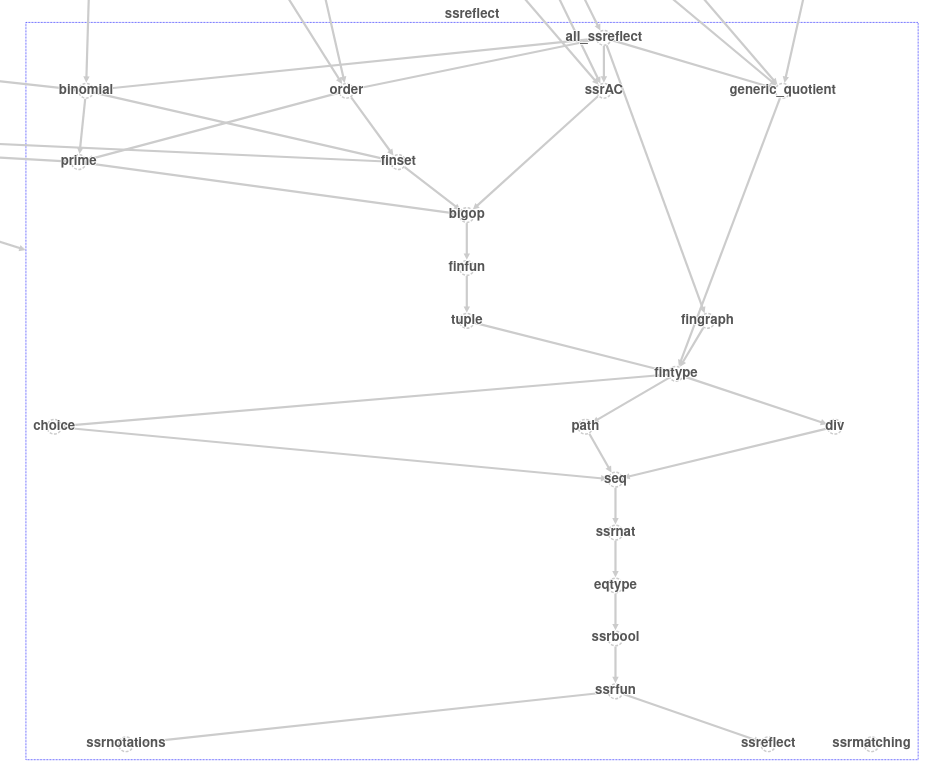
\includegraphics[width=0.6\textwidth]{Figuras/ssreflect.png}\\
    \footnotesize{Disponível em: <\url{https://math-comp.github.io/htmldoc_2_2_0/libgraph.html}>.
    Acesso em: 18 de maio de 2024.}
    \label{fig:graph-mathcomp}
\end{figure}

Os módulos principais para o desenvolvimento da prova sobre o algoritmo Tonelli-Shanks (com base no conteúdo de Teoria dos Números que sustenta a lógica do mesmo) são: \textit{all\_ssreflect} (que contém diversos outros módulos), \textit{ring\_quotient}, \textit{zmodp} e \textit{intdiv}.

\section{Igualdades}
Na maior parte dos teoremas das bibliotecas nativas de \textit{Coq}, usa-se uma definição indutiva de igualdade, que é por sua vez equivalente a igualdade de Leibniz (isto pode ser provado). Por sua vez, essa definição de igualdade é dada pela seguinte proposição indutiva (de acordo com a documentação\footnote{\url{https://coq.inria.fr/doc/V8.18.0/refman/proofs/writing-proofs/equality.html}} \cite{coqteam2022manual}):
    \begin{lstlisting}[language=coq,frame=single,tabsize=1]
Inductive eq {A : Type} (x : A) : A -> Prop := eq_refl : eq x x.
    \end{lstlisting}

De maneira distinta, a biblioteca Mathematical Components, em suas definições e teoremas, utiliza com frequência predicados booleanos \cite{assia_mahboubi_2022_7118596}, que são basicamente funções cujo tipo de retorno é \lstinline[language = coq]!bool!, para então representar proposições da forma \lstinline[language = coq]$x = true$, onde \lstinline[language = coq]$x$ é uma expressão cujo retorno é do tipo \lstinline[language = coq]!bool!. Tais proposições são construídas pela função \lstinline[language = coq]$is_true$.No entanto, através do comando \lstinline[language = coq]$Coercion$ (que será explicado mais detalhadamente adiante neste documento) e por questões de legibilidade, tal função é omitida e o sistema de tipos de \textit{Coq} é capaz de inferir quando uma expressão deve ter tipo \lstinline[language = coq]$bool$ ou tipo \lstinline[language = coq]$Prop$ (e então há uma aplicação de \lstinline[language = coq]$is_true$ omitida). 

Semelhantes aos teoremas existentes para proposição comuns, estão disponíveis diversos teoremas para proposições geradas com o uso de \lstinline[language = coq]$is_true$, como por exemplo o lema \lstinline[language = coq]$contraLR$. Esse é uma versão da contraposição utilizando predicados booleanos (junto à função \lstinline[language = coq]$is_true$) e sua definição é dada por:
    \begin{lstlisting}[language=coq,frame=single,tabsize=1]
Lemma contraLR (c b : bool) : (~~ c -> ~~ b) -> b -> c.
    \end{lstlisting}
onde \lstinline[language = coq]$~~$ é a operação de negação definida na biblioteca Mathematical Components.

Outra informação relevante ao se tratar do conteúdo da biblioteca é o tipo \lstinline[language = coq]$eqType$: para que seja construído qualquer habitante desse tipo é necessário um elemento \lstinline[language = coq]$T$ de tipo 
\lstinline[language = coq]$Type$, uma função \lstinline[language = coq]$eq_op$ de tipo \lstinline[language = coq]$T -> T -> bool$
e um elemento \lstinline[language = coq]$eqP$ cujo tipo é um teorema relacionando a igualdade de Leibniz com \lstinline[language = coq]$T$ e \lstinline[language = coq]$eq_op$. Este último possui, na biblioteca, uma notação de nome \lstinline[language = coq]$eq_axiom$, e sua descrição é:
    \begin{lstlisting}[language=coq,frame=single,tabsize=1]
Definition eq_axiom: forall (T : Type) (e : rel T), forall x x0 : T, 
    reflect (x = x0) (e x x0)
    \end{lstlisting}
onde \lstinline[language = coq]$rel T$ é equivalente ao tipo \lstinline[language = coq]$T -> T -> bool$.

Portanto, para que um tipo \lstinline[language = coq]$A$
pertença ao primeiro campo mencionado, é necessário que se tenha uma prova da proposição \lstinline[language = coq]$eq_axiom A$, isto é, 
a definição \lstinline[language = coq]$eq_axiom$ com 
\lstinline[language = coq]$T$ igual a \lstinline[language = coq]$A$.
Tal teorema indica que a igualdade sobre \lstinline[language = coq]$A$
é decidível, o que fica claro pelo seguinte lema:
    \begin{lstlisting}[language=coq,frame=single,tabsize=1]
Lemma decP: forall (P : Prop) (b : bool), reflect P b -> decidable P
    \end{lstlisting}

A utilização de um tipo como \lstinline[language = coq]$eqType$ facilita que se provem teoremas genéricos, no sentido de que servem para diferentes tipos (pertencentes a \lstinline[language = coq]$Type$) desde que estes possuam uma relação de equivalência decidível. Existem outros tipos semelhantes a \lstinline[language = coq]$eqType$, no sentido de que servem como interfaces. Em grande parte, esses são implementados por meio do açúcar sintático \lstinline[language = coq]$Record$, qual será explicado na sessão seguinte.

\section{Structures e Records} 
\label{section:structs-e-records}

\lstinline[language = coq]$Structure$ e \lstinline[language = coq]$Record$ são comandos sinônimos para geração de tipos indutivos que possuem somente um construtor e cujo os campos são dependentemente tipados, isto é, o tipo de cada campo pode depender dos valores de campos anteriores, assim como nas definições indutivas \cite{assia_mahboubi_2022_7118596}. A vantagem do uso desses comandos é que por meio desses são geradas automaticamente funções para extrair valores dos argumentos do construtor do tipo declarado.

Estes comandos são frequentemente utilizados na biblioteca Mathematical Components para definir interfaces (como o \lstinline[language = coq]$eqType$) e subtipos (ex.: tipo em que os habitantes são todos os números naturais menores que $8$). Para melhor entendimento do leitor, tem-se a seguir um exemplo semelhante ao tipo \lstinline[language = coq]$eqType$ definido na biblioteca, apresentado em \cite{assia_mahboubi_2022_7118596}:
    \begin{lstlisting}[language=coq,frame=single,tabsize=1]
Record eqType : Type := Pack
{
    sort : Type;
    eq_op : sort -> sort -> bool;
    axiom : eq_axiom eq_op
}.
    \end{lstlisting}
Como explicado acima, essa declaração é equivalente a se fazer as seguintes declarações:
    \begin{lstlisting}[language=coq,frame=single,tabsize=1]
Inductive eqType : Type :=
    | Pack (sort : Type) (eq_op : sort -> sort -> bool) (axiom : eq_axiom eq_op).
    
Definition sort (e : eqType) : Type :=
    match e with
    | Pack t _ _ => t
    end.
Definition eq_op (e : eqType) : (sort e -> sort e -> bool) :=
    match e with
    | Pack _ f _ => f
    end.
Definition axiom (e : eqType) : (eq_axiom (eq_op e)) :=
    | Pack _ _ a => a
    end.
    \end{lstlisting}
Observe que o uso de tipos dependentes ocorre nos campos \lstinline[language = coq]{eq_op} e \lstinline[language = coq]{axiom}. No primeiro, o tipo do campo depende do valor do campo \lstinline[language = coq]{sort} e no segundo o tipo do campo depende do valor do campo \lstinline[language = coq]{eq_op} e portanto também do campo \lstinline[language = coq]{sort}.

\subsection{Comando Canonical} Assim como apresentado em \cite{assia_mahboubi_2022_7118596}, para instanciar um habitante de \lstinline[language = coq]$eqType$ com campo \lstinline[language = coq]$sort$ igual a \lstinline[language = coq]$nat$, deve-se provar o seguinte teorema:
    \begin{lstlisting}[language=coq,frame=single,tabsize=1]
Theorem axiom_nat: eq_axiom eqn.
    \end{lstlisting}
onde \lstinline[language = coq]$eqn$ é uma operação de comparação booleana entre números naturais.
Tendo esta prova, podemos instanciar tal habitante
da seguinte forma:
    \begin{lstlisting}[language=coq,frame=single,tabsize=1]
Definition natEqtype := Pack nat eqn axiom_nat.
    \end{lstlisting}
Note que, agora, pode-se comparar dois números naturais da seguinte maneira:
    \begin{lstlisting}[language=coq,frame=single,tabsize=1]
Compute (@eq_op natEqType 2 2).
    \end{lstlisting}
o que nesse caso equivale a:
    \begin{lstlisting}[language=coq,frame=single,tabsize=1]
Compute (eqn 2 2).
    \end{lstlisting}

Entretanto, o objetivo de criar o tipo \lstinline[language = coq]$eqType$ não é estabelecer essa possibilidade de computação para relações de comparação, mas sim construir definições, funções e provas genéricas para todos os tipos que pertencem ao campo \lstinline[language = coq]$sort$ de algum habitante de \lstinline[language = coq]$eqType$ e estabelecer \textit{overloading} de notações. Para exemplo de como alcançar este último objetivo, se define uma notação da seguinte forma:

    \begin{lstlisting}[language=coq,frame=single,tabsize=1]
Notation "x == y" := (@eq_op _ x y).
    \end{lstlisting}
porém havendo apenas esta definição, caso executado o comando \lstinline[language = coq]$Check (3 == 2)$ tem-se um falha. Ao se executar:
    \begin{lstlisting}[language=coq,frame=single,tabsize=1]
Fail Check (3 == 2).
    \end{lstlisting}
a seguinte mensagem é apresentada:
    \begin{lstlisting}[language=coq-error,frame=single,tabsize=1]
The command has indeed failed with message:
The term "3" has type "nat" while it is 
expected to have type "sort ?e"
    \end{lstlisting}
Isto ocorre pois o \textit{Coq} não é capaz de inferir o argumento implícito\footnote{Note que o comando \lstinline[language = coq]$Fail Check (3 == 2)$ é equivalente a \lstinline[language = coq]$Fail Check (@eq_op _ 3 2)$.}  (\lstinline[language = coq]$_$).

Note que é mencionada uma variável \lstinline[language = coq]$?e$. Essa representa um elemento a ser inferido de modo que o tipo \lstinline[language = coq]$sort ?e$ seja igual ao tipo \lstinline[language = coq]$nat$. Como exposto em \cite{10.1007/978-3-642-39634-2_5} o algoritmo de inferência do \textit{Coq} não é capaz de descobrir o valor de tal variável por meio das regras de inferência que possui. Para resolver este problema 
o \textit{Coq} permite que se adicione regras de inferência de tipo por meio do comando \lstinline[language = coq]$Canonical$ (que recebe um construtor de algum \lstinline[language = coq]$Record$ ou \lstinline[language = coq]$Structure$ aplicado aos seus argumentos). Assim, resolver esse problema é possível por meio do seguinte código:
    \begin{lstlisting}[language=coq,frame=single,tabsize=1]
Canonical natEqType.
    \end{lstlisting}
Com isto, de maneira semelhante ao exemplo exposto em \cite{10.1007/978-3-642-39634-2_5}, é adicionada a seguinte regra de inferência ao algoritmo presente em \textit{Coq}:

\begin{equation*}
        \inferrule 
        {
        \text{\lstinline[language = coq]!nat!} \sim 
        \text{\lstinline[language = coq]!sort natEqType!} 
        \\
        \; \text{\lstinline[language = coq]!?!} \text{\lstinline[language = coq]!e!} \; \sim
        \text{\lstinline[language = coq]!natEqType!} 
        }
        {\text{\lstinline[language = coq]!nat!} \sim \text{\lstinline[language = coq]!sort ?e!}}   
\end{equation*}
em que a notação $\sim$ representa uma chamada do algoritmo de unificação \cite{10.1007/978-3-642-39634-2_5} (que é o nome dado ao algoritmo de comparação de tipos chamado nas rotinas de inferência de tipos). Neste momento o leitor pode se perguntar como tal regra de inferência leva o algoritmo a chegar em um resultado final, e a resposta de acordo \cite{10.1007/978-3-642-39634-2_5} está em na existência de outras regras de inferência, como \textit{eq} e \textit{assign}:
\begin{equation*}
    \inferrule
    { }
    {
        \text{\lstinline[language = coq]!t!} \sim \text{\lstinline[language = coq]!t!}
    } \textit{eq}
    \hspace{20mm} % \text{&&}
    \inferrule
    { }
    {
        \text{\lstinline[language = coq]!?!\lstinline[language = coq]!x!} \sim \text{\lstinline[language = coq]!t!}
    } \textit{assign}
\end{equation*}
Retornando ao comando \lstinline[language = coq]$Check$, se agora esse for executado da mesma maneira feita anteriormente (porém sem o \lstinline[language = coq]$Fail$):
    \begin{lstlisting}[language = coq,frame=single,tabsize=1]
Check (3 == 2).
    \end{lstlisting}
tem-se o seguinte resultado:
    \begin{lstlisting}[language = coq-error,frame=single,tabsize=1]
3 == 2
    : bool
    \end{lstlisting}

Como mencionado previamente o tipo \lstinline[language = coq]$eqType$ serve para diversas generalizações. Para exemplo disso, adiante se apresenta a definição de uma comparação entre valores do tipo \lstinline[language = coq]$option$. Antes desse exemplo, vale aqui relembrar o leitor da definição deste tipo:
    \begin{lstlisting}[language = coq,frame=single,tabsize=1]
Inductive option (A : Type) : Type :=
    | None : option A
    | Some : A -> option A.
    \end{lstlisting}
A função de comparação a ser declarada irá considerar que o argumento \lstinline[language = coq]$A$ pertence ao campo \lstinline[language = coq]$sort$ de algum habitante de \lstinline[language = coq]$eqType$. Tem-se então a definição dessa função:
    \begin{lstlisting}[language = coq,frame=single,tabsize=1]
Definition cmp_option (e : eqType) (o1 o2 : option (sort e)) :=
    match o1, o2 with
    | Some e1, Some e2 => op e e1 e2
    | None, Some _ => false
    | Some _, None => false
    | None, None => true
    end.
    \end{lstlisting}
Agora, para criar um habitante de \lstinline[language = coq]$eqType$ para todo tipo da forma \lstinline[language = coq]$option A$ (note que para todo \lstinline[language = coq]$A$ diferente tem-se um tipo diferente) em que o tipo \lstinline[language = coq]$A$ segue o que foi considerado na função, deve-se provar o seguinte teorema:
    \begin{lstlisting}[language = coq,frame=single,tabsize=1]
Theorem axiom_option: 
    forall e : eqType, eq_axiom (cmp_option e).
    \end{lstlisting}
que para facilidade de entendimento do leitor, pode ser escrito como:
    \begin{lstlisting}[language = coq,frame=single,tabsize=1]
Theorem axiom_option: 
    forall e : eqType, forall x y : option (sort e), reflect (x = y) (@cmp_option e x y).
    \end{lstlisting}
Com esta prova pode-se construir a seguinte definição:
    \begin{lstlisting}[language = coq,frame=single,tabsize=1]
Definition optionEqType (e : eqType) := 
    Pack (option (sort e)) (cmp_option e) (axiom_option e).
    \end{lstlisting}
Visto que ainda não foi executado o comando \lstinline[language = coq]$Canonical$ com esta definição, se executado o comando \lstinline[language = coq]$Check (Some 1 == Some 2)$, esse irá falhar, logo, ao se executar:
    \begin{lstlisting}[language = coq,frame=single,tabsize=1]
Fail Check (Some 1 == Some 2).
    \end{lstlisting}
É apresentada a seguinte mensagem:
    \begin{lstlisting}[language = coq-error,frame=single,tabsize=1]
The command has indeed failed with message:
The term "Some 1" has type "option nat" 
while it is expected to have type "sort ?e".
    \end{lstlisting}
Semelhante ao que foi feito anteriormente, para resolver este problema deve-se executar: 
    \begin{lstlisting}[language = coq,frame=single,tabsize=1]
Canonical optionEqType.
    \end{lstlisting}
e com isso se adiciona a seguinte regra de inferência:
% Semelhante ao que foi feito anteriormente, para resolver este problema deve-se executar: 
%     \begin{lstlisting}[language = coq,frame=single,tabsize=1]
% Canonical optionEqType.
%     \end{lstlisting}
% e com isso se adiciona a seguinte regra de inferência:
\begin{equation*}
    \inferrule
    {
    \text{\lstinline[language = coq]!t!} \sim 
    \text{\lstinline[language = coq]!sort ?x!} 
    \\ 
    \text{\lstinline[language = coq]!?!\lstinline[language = coq]!e!} \sim
    \text{\lstinline[language = coq]!optionEqType ?x!} 
    }
    {
        \text{\lstinline[language = coq]!option t!} \sim \text{\lstinline[language = coq]!sort ?e!}
    }   
\end{equation*}
Assim note que no problema de inferência acima, ocorre a seguinte (sub)sequência de aplicação de regras de inferência para se determinar o valor de \lstinline[language = coq]$?e$:
\begin{equation*}
    \inferrule []
    {
        \inferrule []
        {
        \text{\lstinline[language = coq]!nat!} \sim 
        \text{\lstinline[language = coq]!sort natEqType!} 
        \\ 
        \text{\lstinline[language = coq]!?!\lstinline[language = coq]!x!} \sim
        \text{\lstinline[language = coq]!natEqType!} 
        }
        {\text{\lstinline[language = coq]!nat!} \sim \text{\lstinline[language = coq]!sort ?x!}} 
        % \lstinline[language = coq]!nat! \sim 
        % \lstinline[language = coq]!sort ?x! 
        \\ 
        \\
        \text{\lstinline[language = coq]!?!\lstinline[language = coq]!e!} \sim
        \text{\lstinline[language = coq]!optionEqType ?x!} 
    }
    {\text{\lstinline[language = coq]!option nat!} \sim \text{\lstinline[language = coq]!sort ?e!}}   
\end{equation*}
Agora, com o comando:
    \begin{lstlisting}[language = coq,frame=single,tabsize=1]
Check (Some 1 == Some 2).
    \end{lstlisting}
tem-se a mensagem:
    \begin{lstlisting}[language = coq-error,frame=single,tabsize=1]
Some 1 == Some 2
    : bool
    \end{lstlisting}

\subsection{Comando Coercion} \label{subsection:coercion}

Em provas manuais costuma-se utilizar notações iguais para operações sobre diferentes tipos. Como exemplo, há o uso do símbolo $+$ para operação de soma sobre os conjuntos númericos $\mathbb{N}$, $\mathbb{Z}$, $\mathbb{Q}$, $\mathbb{R}$ , como operador lógico \textit{ou} e também como operação binária qualquer que forma um monoide genérico. Nessa aplicação cotidiana de \textit{overloading} de notações, as informações sobre tipos são inferidas pelo cérebro humano conforme o contexto em que se encontram \cite{10.1007/978-3-642-39634-2_5}. 
Tomando isso em consideração e tendo em mente o conteúdo abordado na subseção anterior, pode-se dizer que o comando \lstinline[language = coq]$Canonical$ auxilia os usuários, tornando a escrita em \textit{Coq} mais semelhante a que se faz manualmente.

Outro mecanismo relacionado a tipos em \textit{Coq}, e que de certa forma serve para esse mesmo propósito, é provido pelo comando \lstinline[language = coq]$Coercion$. Como motivação para o uso deste, suponha a declaração em \textit{Coq} de um tipo que contenha todos os números naturais múltiplos de um número $n$. Utilizando \lstinline[language = coq]$Record$, temos então: 
    \begin{lstlisting}[language = coq,frame=single,tabsize=1]
Record multiple (n : nat) : Type := Build
{       
    x : nat;
    axiom : (n %| x)        
}.
    \end{lstlisting}
Observe que para construir um habitante deste tipo é dado um elemento \lstinline[language = coq]$n$ de tipo \lstinline[language = coq]$nat$ e é necessário um elemento \lstinline[language = coq]$x$ de mesmo tipo, e além disso, uma prova\footnote{Há de maneira implícita a aplicação da função \lstinline[language = coq]$is_true$ no tipo do campo \lstinline[language = coq]$axiom$, portanto o que foi declarado como tipo deste campo, isto é, \lstinline[language = coq]$n \%| x$, é equivalente a \lstinline[language = coq]$n \%| x = true$.} de que \lstinline[language = coq]$x$ é divisível por \lstinline[language = coq]$n$.
Agora, com tal declaração, visto que o objetivo da mesma é representar qualquer conjunto de números divisíveis por um determinado natural $n$, o usuário de \textit{Coq} provavelmente desejará que se possa escrever algo como:
    \begin{lstlisting}[language = coq,frame=single,tabsize=1]
forall (n : nat) (a : multiple n), a + 0 = a.
    \end{lstlisting}
sem que o uso da operação de adição leve a um erro pela razão dessa possuir tipo \lstinline[language = coq]$nat -> nat -> nat$ enquanto o argumento \lstinline[language = coq]$a$ tem tipo \lstinline[language = coq]$multiple n$, quando a intenção do usuário é de que este último represente um número natural. Se for utilizado o comando \lstinline[language = coq]$Check$ na proposição acima:
    \begin{lstlisting}[language = coq,frame=single,tabsize=1]
Fail Check (forall (n : nat) (a : multiple n), a + 0 = a).
    \end{lstlisting}
tem-se a mensagem:
    \begin{lstlisting}[language = coq-error,frame=single,tabsize=1]
The command has indeed failed with message:
In environment
n : nat
a : multiple n
The term "a" has type "multiple n" while it is
expected to have type "nat".
    \end{lstlisting}
Buscando solucionar este tipo de problema, sem que tenha que se escrever:
    \begin{lstlisting}[language = coq,frame=single,tabsize=1]
forall (n : nat) (a : multiple n), (x n a) + 0 = (x n a).
    \end{lstlisting}
o que por sua vez não geraria erro algum pois \lstinline[language = coq]$(x n a)$ tem tipo \lstinline[language = coq]$nat$\footnote{Lembre-se que \lstinline[language = coq]$x$, no contexto externo a declaração do seu respectivo \lstinline[language = coq]$Record$, é uma função que extrai o campo \lstinline[language = coq]$x$ de um elemento do tipo \lstinline[language = coq]$multiple n$ (para qualquer \lstinline[language = coq]$n$) e não o valor do campo em si. Portanto a seguinte definção poderia ser dada simplesmente como \lstinline[language = coq]$x$.}, defini-se uma função que retira o campo \lstinline[language = coq]$x$ de um elemento como \lstinline[language = coq]$a$:
    \begin{lstlisting}[language = coq,frame=single,tabsize=1]
Definition multiple_nat (n : nat) (e : multiple n) : nat :=
    let t := (x n e) in t.
    \end{lstlisting}
e agora, para que o \textit{Coq} aplique esta função de maneira implícita, de modo a evitar erros de tipo, usa-se o comando \lstinline[language = coq]$Coercion$ da seguinte maneira:
    \begin{lstlisting}[language = coq,frame=single,tabsize=1]
Coercion multiple_nat : multiple >-> nat.
    \end{lstlisting}
Agora, realizando o comando \lstinline[language = coq]$Check$ como anteriormente:
    \begin{lstlisting}[language = coq,frame=single,tabsize=1]
Check (forall n (a : multiple n), a + 0 = 0).
    \end{lstlisting}
é gerada a mensagem:
    \begin{lstlisting}[language = coq-error,frame=single,tabsize=1]
forall (n : nat) (a : multiple n), a + 0 = 0
    : Prop
    \end{lstlisting}

\subsection{Exemplo de Implementação de grupos}
\label{sub:grupos}

Um uso semelhante do mecanismo \textit{coercion}, junto ao \textit{canonical}, pode ser proposto com um tipo que representa grupos. Um grupo é uma estrutura algébrica dada por $(G, \otimes)$ onde:
\begin{enumerate}
    \item $\otimes$ é uma operação binária sobre $G$, isto é, $\otimes$ é uma função tal que $\otimes : (G \times G) \rightarrow G$.
    \item $\otimes$ é associativa, ou seja, $\forall a, b \in G, (a \otimes b) \otimes c = a \otimes (b \otimes c)$.
    \item Existe um elemento neutro $e$, o que significa: $\exists e \in G (\forall a \in G, e \otimes a = a \otimes e = a)$. 
    \item Para todo elemento em $G$ existe um elemento inverso, isto é, \\
    $\forall x \in G (\exists \;\overline{x} \in G, x \;\otimes\; \overline{x} = \overline{x} \;\otimes\; x = e)$
\end{enumerate}
Em \textit{Coq} um grupo pode ser representado pelo seguinte \lstinline[language = coq]$Record$:
    \begin{lstlisting}[language = coq,frame=single,tabsize=1]
Record Group : Type := group 
{
    sort :> Type;
    bin_op : sort -> sort -> sort;
    associative_axiom : associative bin_op;
    e : sort;
    neutral_left : left_id e bin_op;
    neutral_right : right_id e bin_op;
    inverse_left : \forall x : sort, \exists y : sort, bin_op y x = e; 
    inverse_right : \forall x : sort, \exists y : sort, bin_op x y = e 
}.
    \end{lstlisting}
Observe que, diferente dos exemplos anteriores, o campo \lstinline[language = coq]$sort$ é seguido de \lstinline[language = coq]$:>$. Esse operador além de atribuir o tipo de \lstinline[language = coq]$sort$ como \lstinline[language = coq]$Type$
define a função \lstinline[language = coq]$sort$ como uma \textit{coercion} para todo habitante do tipo \lstinline[language = coq]$Group$. Assim, suponha a definição do seguinte habitante:
    \begin{lstlisting}[language = coq,frame=single,tabsize=1]
Definition int_group := 
    Group int addz addzA 0 add0z addz0 inverse_left_int inverse_right_int.
    \end{lstlisting}
Esse habitante tem como campo \lstinline[language = coq]$sort$ o tipo \lstinline[language = coq]$int$ (que representa os números inteiros) e devido a \textit{coercion}, se for feita uma declaração com uma variável de tipo \lstinline[language = coq]$int_group$ em que se aplica uma função de tipo \lstinline[language = coq]$int -> int$ sobre esta variável, o \textit{Coq} irá automaticamente tratar a variável como tendo tipo \lstinline[language = coq]$int$ (ou mais especificamente, irá tratá-la como se fosse o valor de seu campo \lstinline[language = coq]$sort$, aplicando de maneira implícita a função \lstinline[language = coq]$sort$ sobre a mesma).

Para fins de demonstrar uma implentação completa de grupos em \textit{Coq}, define-se agora uma notação para as operações binárias e uma para os elementos neutros que formam grupos quaisquer, da seguinte forma:
    \begin{lstlisting}[language = coq,frame=single,tabsize=1]
Notation "x \otimes y" := (@bin_op _ x y) (at level 10).
Notation "0" := (@e _).
    \end{lstlisting}
Usa-se então o comando \lstinline[language = coq]$Canonical$ para que o \textit{Coq} seja capaz de inferir os argumentos implícitos presentes nas descrições destas notações (para o caso de \lstinline[language = coq]$x$ e  \lstinline[language = coq]$y$ possuirem tipo  \lstinline[language = coq]$int$):
    \begin{lstlisting}[language = coq,frame=single,tabsize=1]
Canonical int_group.
    \end{lstlisting}
Com este conjunto de configurações passa a ser mais fácil a escrita e leitura de declarações relacionadas a grupos. Assim, torna-se então possível a formalização compacta de teoremas genéricos sobre quaisquer tipos presentes no campo \lstinline[language = coq]$sort$ de algum habitante de \lstinline[language = coq]$group$. Como exemplo, tem-se o seguinte teorema e sua respectiva prova:
    \begin{lstlisting}[language = coq,frame=single,tabsize=1]
Theorem exemplo_sobre_grupos: 
    \forall G : group, \forall a b : G, (a \otimes b) \otimes 0 = (a \otimes 0) \otimes b.
Proof.
    intros. rewrite (neutral_right G). rewrite (neutral_right G).
    reflexivity. 
Qed.
    \end{lstlisting}
Como este teorema serve para qualquer grupo \lstinline[language = coq]$G$, esse pode então ser usado na seguinte prova:
    \begin{lstlisting}[language = coq,frame=single,tabsize=1]
Theorem exemplo_sobre_int:
    \forall a b : int, (a + b) + 0 = (a + 0) + b.
Proof.
    apply exemplo_sobre_grupos.
Qed.
    \end{lstlisting}
Tal prova exemplifica como o uso dos mecanismos em \textit{Coq}, que foram apresentados neste capítulo, podem ser utilizados para que seja mais fácil trabalhar com um vasta quantidade de tipos que apresentam propriedades em comum (como é o caso dos grupos).

\subsection{Mantendo Informações de um Record ou Structure}

Em meio as provas que envolvem tipos de \lstinline[language = coq]$Record$ ou \lstinline[language = coq]$Structure$, o usuário de \textit{Coq} pode se deparar com situações em que, ao se aplicar uma determinada função sobre uma variável relacionada a um desses comandos, que portanto apresenta um determinado conjunto de propriedades, o resultado da computação dessa função irá retornar um dado do tipo definido pela \textit{coercion}. Em algumas dessas ocasiões, no entanto, a função aplicada retornará um dado com o qual se poderia construir uma nova variável do mesmo tipo de \lstinline[language = coq]$Record$ (ou \lstinline[language = coq]$Structure$) do elemento do qual o argumento da função foi extraído. Manter o tipo do resultado como o mesmo \lstinline[language = coq]$Record$ ou \lstinline[language = coq]$Structure$ pode ser útil em algumas provas, e fazer isso é possível através do comando \lstinline[language = coq]$Canonical$. A exemplo disso, retomando ao tipo \lstinline[language = coq]$multiple$, note que é possível provar os dois seguintes teoremas:
    \begin{lstlisting}[language = coq,frame=single,tabsize=1]
Theorem exemplo_multiple_axiom {n} :
    \forall (a : multiple n), n %| a.
Theorem exemplo_aplicacao_f_mul {n} :
    \forall (f : nat -> nat) (a : multiple n), n %| (f a) * n.
    \end{lstlisting}
onde \lstinline[language = coq]$%%$ é a operação de resto da divisão. Agora, imagine que se queira provar o seguinte:
    \begin{lstlisting}[language = coq,frame=single,tabsize=1]
Example exemplo_a_provar {n} :
    \forall (a : multiple n), (n %| ((fun x => x + 2) a) * n).
    \end{lstlisting}
Note que, se tratando \lstinline[language = coq]!multiple n! como um conjunto de números naturais (apesar desse não ser precisamente isso) faria sentido poder utilizar o teorema \lstinline[language = coq]!exemplo_multiple_axiom! para reescrever o lado esquerdo da equação como \lstinline[language = coq]!true! (o operador  \lstinline[language = coq]!%|! tem tipo \lstinline[language = coq]!nat -> nat -> bool! portanto há uma \textit{coercion} \lstinline[language = coq]!is_true! na declaração do exemplo), ao invés de ter que utilizar um teorema mais específico como \lstinline[language = coq]!exemplo_aplicacao_f_mul!. Dado que se trata de uma aplicação de função em que após a aplicação o resultado é multiplicado por \lstinline[language = coq]!n!, é óbvio que o resultado da expressão:
    \begin{lstlisting}[language = coq,frame=single,tabsize=1]
(((fun x => x + 2) a) * n)
    \end{lstlisting} 
é divisível por \lstinline[language = coq]!n!. Entretanto, a reescrita desejada não é possível pois ocorre um problema de unificação ao tentar se usar a tática \lstinline[language = coq]!rewrite exemplo_multiple_axiom!. Para obter-se uma melhor noção sobre este problema é possível utilizar o seguinte código fornecido por \cite{assia_mahboubi_2022_7118596} (sobre o qual a explicação de seu funcionamento vai além do escopo do presente trabalho):
    \begin{lstlisting}[language = coq,frame=single,tabsize=1]
Notation "X (*...*)" :=
    (let x := X in let y := _ in x) (at level 100, format "X  (*...*)").

Notation "[LHS 'of' equation ]" := 
    (let LHS := _ in let _infer_LHS := equation : LHS = _ in LHS) (at level 4).

Notation "[unify X 'with' Y ]" := 
    (let unification := erefl _ : X = Y in True).
    \end{lstlisting} 
Com isso, pode-se executar o seguinte comando:
    \begin{lstlisting}[language = coq,frame=single,tabsize=1]
Fail Check (forall n (a : multiple n) (f : nat -> nat),
    let LHS := [LHS of exemplo_multiple_axiom _] in
    let RDX := (n %| (f a) * n) in
    [unify LHS with RDX]).
    \end{lstlisting}
Este comando irá apresentar uma mensagem de confirmação da falha, que em parte, apresenta o seguinte conteúdo:
    \begin{lstlisting}[language = coq-error,frame=single,tabsize=1]
The command has indeed failed with message:
In environment
n :
nat
a : multiple n
f : nat -> nat
LHS := [LHS of exemplo_multiple_axiom ?a] : bool
RDX := n %| f (x n a) * n : bool
The term "erefl LHS" has type "LHS = LHS"
while it is expected to have type "LHS = RDX"
    \end{lstlisting} 
Com isto, pode-se verificar que o problema de unificação encontrado é descobrir qual o valor da variável \lstinline[language = coq]!?a!. De modo mais específico, o problema está em encontrar um valor que torne equivalentes as seguintes expressões:
    \begin{lstlisting}[language = coq,frame=single,tabsize=1]
n %| (x n ?a)
    \end{lstlisting} 
e
    \begin{lstlisting}[language = coq,frame=single,tabsize=1]
n %| ((f (x n a)) * n)
    \end{lstlisting}
 Para resolver este problema % e então simular tal tratamento de \lstinline[language = coq]!smaller n! como um conjunto (para este caso em específico) em \textit{Coq}, 
 usa-se o comando \lstinline[language = coq]!Canonical! junto ao teorema\\ 
 \lstinline[language = coq]!exemplo_aplicacao_f_mul!, através do seguinte código:
    \begin{lstlisting}[language = coq,frame=single,tabsize=1]
Canonical f_mul_multiple {n : nat} (f : nat -> nat) (a : multiple n) := 
    (@Build n ((f a) * n) (@exemplo_aplicacao_f_mul n f a)).
    \end{lstlisting} 
    Retornando então a prova de motivação para introdução ao problema discutido\\
    (\lstinline[language = coq]!exemplo_a_provar!) e utilizando a tática:
    \begin{lstlisting}[language = coq,frame=single,tabsize=1]
intros. simpl.
    \end{lstlisting} 
O \textit{goal} da prova se torna:
    \begin{lstlisting}[language = coq,frame=single,tabsize=1]
n %| (a + 2) * n
    \end{lstlisting}
Agora, para que se possa aplicar novamente a tática \lstinline[language = coq]!rewrite exemplo_smaller_axiom!, é necessário deixar o \textit{goal} escrito de modo que a expressão mais interna:
    \begin{lstlisting}[language = coq,frame=single,tabsize=1]
(a + 2)
    \end{lstlisting}
fique na forma de uma função aplicada sobre um elemento múltiplo de \lstinline[language = coq]!n!.
Isso é necessário para que o \textit{Coq} possa inferir um elemento do tipo \lstinline[language = coq]!multiple n! dado pela definição \lstinline[language = coq]!f_mul_multiple!, permitindo assim o uso do teorema \lstinline[language = coq]!exemplo_multiple_axiom!. Como \lstinline[language = coq]!2! é de tipo \lstinline[language = coq]!nat!, o \textit{Coq} não consegue construir um habitante do tipo \lstinline[language = coq]!multiple n! que resolva o problema de unificação. O que se pode então fazer é inverter a ordem da função de soma, realizando a tática \lstinline[language = coq]!rewrite addnC!, em que \lstinline[language = coq]!addnC! é um teorema de comutativa da soma. Assim, o \textit{goal} resultante será:
    \begin{lstlisting}[language = coq,frame=single,tabsize=1]
n %| ((2 + a) * n)
    \end{lstlisting}
Agora, utilizando novamente a tática \lstinline[language = coq]!rewrite exemplo_multiple_axiom!, tem-se:
    \begin{lstlisting}[language = coq,frame=single,tabsize=1]
true
    \end{lstlisting}
Com isso a prova pode ser finalizada com o uso de 
\lstinline[language = coq]!reflexivity!.
	\chapter{Base Teórica}
\label{cap:base}

Para que se realizem as implementações serão necessários diversos teoremas, lemas e funções, dos quais, parte, já estão implementados na biblioteca Mathematical Components. Sendo assim, o presente capítulo busca trazer a descrição da maioria destes itens, colocando também suas respectivas implementações disponíveis na biblioteca (se houver). 

A maior parte do conteúdo deste capítulo se baseia no livro \cite{book:2399854}, que foi amplamente estudado para realização deste trabalho. Sendo assim, as provas não apresentadas aqui se encontram nesse livro.

\section{Máximo Divisor Comum}
Tendo sido apresentado os conceitos de módulo e divisibilidade, outro pilar fundamental da Teoria dos Números é o conceito de $\mdc$ (máximo divisor comum). A princípio, a definição seria auto-explicativa, mas parte de diversos teoremas importantes a utiliza e portanto é interessante que se tenha uma definição equivalente específica para facilitar provas futuras. Para se obter tal definição alternativa, observe que, formalmente, a definição de $\mdc$ é:
    \begin{equation*}
        \forall a, b, n \in \mathbb{Z},  \mdc(a, b) = n \Leftrightarrow (n \mid a) \land (n \mid b) \land (\forall k \in \mathbb{Z}, (k \mid a) \land (k \mid b) \rightarrow k \leq n)
    \end{equation*}
Analisando a proposição:
    \begin{equation*}
        \forall k \in \mathbb{Z}, (k \mid a) \land (k \mid b) \rightarrow k \leq n
    \end{equation*}
Pode-se verificar os seguintes casos:
    \begin{enumerate}
        \item $|k| = |n|$, isto é, $k = n$ ou $k = -n$. Em ambos estes casos $k \mid n$.

        \item $|k| < |n|$, assim, como $n \mid a$ e $n \mid b$, então, $\exists q_a, q_b \in \mathbb{Z}, (a = q_a \cdot n \land b = q_b \cdot n) $, onde $\mdc(q_a, q_b) = 1$ (caso contrário $n$ não seria $\mdc(a,b)$, pois haveria o divisor $\mdc(q_a, q_b) \cdot n$ que é maior que $n$, se $n > 1$). Portanto, como $k \mid a$ e $k \mid b$, então $k \mid q_a \cdot n$ e $k \mid q_b \cdot n$, mas sabe-se que $k \nmid q_a$ e $k \nmid q_b$, logo, $k \mid n$.
    \end{enumerate}
Olhando o que acontece quando $k \mid n$, é fácil notar que $|k| \leq |n|$, logo, no contexto em que $k \mid a$ e $k \mid b$, as afirmações $k \leq n$ e $k \mid n$ são equivalentes. Sendo assim tem-se a seguinte definição alternativa:
\begin{equation*}
        \forall k \in \mathbb{Z}, (k \mid a) \land (k \mid b) \rightarrow k \mid n
\end{equation*}    

\section{Algoritmo de Euclides}
\label{sec:algoritmo-de-euclides}

O algoritmo de Euclides é um método de computar o $\mdc$ entre dois números inteiros $a$ e $b$, tendo a seguinte descrição (Algoritmo \ref{algo:euclides}):

        \begin{algorithm}[!htbp]
                \SetAlgoLined
                \vspace{3mm}
                \Entrada{$a, b \in \mathbb{Z}$}
                \Saida{inteiro $n$.}
                \Se{$a = 0$}
                {\Retorna{$b$}}
                \SeN
                {\Retorna{\hyperref[algo:euclides]{\textsc{Euclides}}($b$, $a\bmod b$)}}
                \caption{\textsc{Euclides}}\label{algo:euclides}
        \end{algorithm}

\noindent
Este algoritmo se baseia no seguinte lema:
\begin{lema} \label{lema:euclides}
    $\forall a, b \in \mathbb{Z}$, seja $a = b \cdot q  + r$, onde $0 \leq r < |b|$, então:
    \begin{equation*}
        \mdc(a, b) = \mdc(b, r)
    \end{equation*}
\end{lema}
    % \begin{proof}
\noindent
\textit{Demonstração}: inicialmente deve-se notar que, provar tal lema equivale a demonstrar:
        \begin{equation} \label{eq : 1}
            \forall n \in \mathbb{Z}, (\mdc(a, b) = n \leftrightarrow \mdc(b, r) = n)
        \end{equation}
        Além disso, deve-se considerar o seguinte lema trivial que versa sobre combinações lineares:
        \begin{lema}[\textit{Divisibilidade e combinações lineares}]
            \begin{equation*}
                \forall a, b, n \in \mathbb{Z}, (n \mid a) \land (n \mid b) \rightarrow \forall c_1, c_2 \in \mathbb{Z}, n \mid (c_1 \cdot a + c_2 \cdot b)
            \end{equation*}
        \end{lema}
        Dados esses adendos, prova-se inicialmente a volta da bi-implicação \ref{eq : 1}. Para isso, observe que, se $x = \mdc(b, r)$ então $x \mid b$ e $x \mid r$, e como $r = a - b \cdot q$ então $x \mid (a - b \cdot q)$. Pode-se então fazer uma combinação linear escolhendo $c_1 = q$ e $c_2 = 1$, donde se chega em:
        \begin{equation*}
                x \mid q \cdot b + 1 \cdot (a - b \cdot q)
        \end{equation*}
        \begin{equation*}
                x \mid q \cdot b + a - b \cdot q
        \end{equation*}
        \begin{equation*}
                x \mid a
        \end{equation*}
        Resta então provar que:
        \begin{equation*}
            \forall y \in \mathbb{Z}, (y \mid a) \land (y \mid b) \rightarrow (y \mid x) 
        \end{equation*}
        Da hipótese tem-se que
        \begin{equation*}
            \forall y \in \mathbb{Z}, (y \mid b) \land (y \mid r) \rightarrow (y \mid x) 
        \end{equation*}
        Se $y \mid a$ e $y \mid b$, como $a = b \cdot q + r$ então
        $y \mid (b \cdot q + r)$. Utilizando o teorema sobre combinação linear novamente, com $c_1 = -q$ e $c_2 = 1$:
        \begin{equation*}
            y \mid -q \cdot b + 1 \cdot (b \cdot q + r) 
        \end{equation*}
        \begin{equation*}
            y \mid - b \cdot q + b \cdot q + r 
        \end{equation*}
        \begin{equation*}
            y \mid r 
        \end{equation*}
        Como $y \mid b$ e $y \mid r$, da hipótese temos que $y \mid x$ portanto se provou o que restava. Para a ida da bi-implicação a prova é semelhante. \qed
    % \end{proof}
% \end{lema}

O algoritmo \hyperref[algo:euclides]{\textsc{Euclides}} é implementado da seguinte forma na biblioteca Mathematical Components (em sua versão para números naturais):
    \begin{lstlisting}[language=coq,frame=single,tabsize=1]
Fixpoint gcdn m n :=
    let n' := n %% m in if n' is 0 then m else
    if m - n'.-1 is m'.+1 then gcdn (m' %% n') n' else n'.
    \end{lstlisting}
A versão para números inteiros é basicamente \lstinline[language = coq]{gcdn} aplicada sobre o valor absoluto dos números inteiros de entrada.
% \begin{lstlisting}[language = coq]
%     Definition gcdz m n := (gcdn `|m| `|n|)%:Z.
% \end{lstlisting}
Sobre a notação \lstinline[language = coq] essa representa a operação de resto da divisão, que, para números naturais é definida por:
    \begin{lstlisting}[language=coq,frame=single,tabsize=1]
Definition modn_rec d := 
    fix loop m := if m - d is m'.+1 then loop m' else m.
Definition modn m d := if d > 0 then modn_rec d.-1 m else m.
Notation "m %% d" := (modn m d) : nat_scope.
    \end{lstlisting}
E utilizando a função 
\lstinline[language = coq]{divz} para divisão entre números inteiros, é implementada da seguinte forma (para inteiros):
    \begin{lstlisting}[language=coq,frame=single,tabsize=1]
Definition modz (m d : int) : int := m - divz m d * d.
Infix "%%" := modz : int_scope.
    \end{lstlisting}

\section{Teorema Bachet-Bézout}

Uma das consequências teóricas da definição de $\mdc$ é o Teorma Bachet-Bézout. Este por sua vez traz uma aplicação do conceito de $\mdc$ na resolução de equações. O seu enunciado é dado por:
\begin{teorema}[\textit{Bachet-Bézout}] \label{teorema : bachetbezout}
    $\forall a, b \in \mathbb{Z}, \exists x, y \in \mathbb{Z}$ tal que
    \begin{equation*}
        a \cdot x + b \cdot y = \mdc(a, b)
    \end{equation*}
\end{teorema}
\noindent
Como exemplo de consequências deste teorema têm-se:
\begin{enumerate}
    \item $\forall c \in \mathbb{Z}, c \mid a \land c \mid b \Rightarrow c \mid \mdc(a, b)$, ou seja, caso $c$ divida tanto $a$ quanto $b$ então $c$ divide $\mdc(a, b)$.
    \item $\forall c \in \mathbb{Z}, (\exists x, y \in \mathbb{Z}, a \cdot x + b \cdot y = c) \Longleftrightarrow \mdc(a, b) \mid c $, ou seja, a equação $a \cdot x + b \cdot y = c$ tem solução se e somente se $\mdc(a, b)$ divide $c$.
\end{enumerate}
A prova manual do Teorema \ref{teorema : bachetbezout} e das consequências mencionadas se encontra em \cite{book:2399854}.

    Em relação à biblioteca Mathematical Components e se tratando do Teorema \ref{teorema : bachetbezout}, essa possui a implementação de um algoritmo
    % do algoritmo conhecido como "algoritmo de Euclides extendido" (
    que encontra os coeficientes $x$ e $y$ e o valor de $\mdc(a,b)$. Este algoritmo possui duas versões, sendo identificado na biblioteca como \lstinline[language = coq]{egcdn} para naturais e \lstinline[language = coq]{egcdz} para inteiros. Além disso, existem os lemas \lstinline[language = coq]{egcdn_spec} e \lstinline[language = coq]{egcdz_spec}, tratando da corretude desses algoritmos (respectivamente) e para o caso dos números inteiros, há o lema \lstinline[language = coq]{Bezoutz} que é equivalente ao Teorema \ref{teorema : bachetbezout}.

\section{Propriedades de Congruência}
As propriedade da relação de congruência serão usadas com muita frequência (e de maneira implícita) no decorrer desse documento. Por essa razão, nesta seção serão listadas essas propriedades. Recomenda-se então ao leitor consultar o conteúdo aqui apresentado em caso de dúvidas no desenvolvimento de equações modulares.
    
    Seguindo para as propriedades, para todo $a,b, c, d, n \in \mathbb{Z}$ têm-se:
\begin{enumerate}
    \item (\textit{Reflexividade}) $a \equiv a \pmod{n}$
    \item (\textit{Simetria}) $a \equiv b \pmod{n} \Longrightarrow b \equiv a \pmod{n}$
    \item (\textit{Transitividade}) $a \equiv b \pmod{n} \land b \equiv c \pmod{n} \Longrightarrow a \equiv c \pmod{n}$
    \item (\textit{Compatibilidade com a soma})
    \begin{equation*}
        a \equiv b \pmod{n} \land c \equiv d \pmod{n} \Longrightarrow a + c \equiv b + d \pmod{n}
    \end{equation*}
    \item (\textit{Compatibilidade com a diferença})
    \begin{equation*}
        a \equiv b \pmod{n} \land c \equiv d \pmod{n} \Longrightarrow a - c \equiv b - d \pmod{n}
    \end{equation*}
    \item \label{item:propcong6-produto} (\textit{Compatibilidade com o produto})
    \begin{equation*}
        a \equiv b \pmod{n} \land c \equiv d \pmod{n} \Longrightarrow a \cdot c \equiv b \cdot d \pmod{n}
    \end{equation*}
    A partir dessa propriedade, note que, para todo $k \in \mathbb{N}$:
    \begin{equation*}
        a \equiv b \pmod{n} \Longrightarrow a^k \equiv b^k \pmod{n}
    \end{equation*}
    \item \label{item:propcong7-cancelamento} (\textit{Cancelamento}) $\mdc(c, n) = 1 \Longrightarrow (a \cdot c \equiv b \cdot c \pmod{n} \Longleftrightarrow a \equiv b \pmod{n})$   
\end{enumerate}

Na biblioteca Mathematical Components, as relações de módulo são definidas pelas seguintes notações:
    \begin{lstlisting}[language=coq,frame=single,tabsize=1]
Notation "m = n %[mod d ]" := (modz m d = modz n d) : int_scope.
Notation "m == n %[mod d ]" := (modz m d == modz n d) : int_scope.
Notation "m <> n %[mod d ]" := (modz m d <> modz n d) : int_scope.
Notation "m != n %[mod d ]" := (modz m d != modz n d) : int_scope.
    \end{lstlisting}
Deve-se observar que existem duas igualdades, sendo a primeira a de Leibniz e a segunda uma função booleana. O mesmo ocorre com as desigualdades (na mesma ordem).

Tais definições são equivalentes a definição apresentada por \cite{book:2399854}, conforme é mostrado pelo lema \lstinline[language = coq]{eqz_mod_dvd} implementado na biblioteca \footnote{O operador 
\lstinline[language = coq]{\%Z} serve para indicar o escopo da operação dentro do parênteses}:
    \begin{lstlisting}[language=coq,frame=single,tabsize=1]
Lemma eqz_mod_dvd d m n : (m == n %[mod d])%Z = (d %| m - n)%Z.
    \end{lstlisting}

Quanto a implementação das propriedades apresentadas nesta seção, a biblioteca não as implementa, apesar de fazer isso para lemas semelhantes a algumas destas propriedades. A exemplo tem-se:
    \begin{lstlisting}[language=coq,frame=single,tabsize=1]
Lemma modzDm m n q : ((m %% q)%Z + (n %% q)%Z = m + n %[mod q])%Z.
    \end{lstlisting}
Este lema se assemelha a propriedade de \textit{compatibilidade com a soma}, no sentido de que, considerando a existência do seguinte lema:
    \begin{lstlisting}[language=coq,frame=single,tabsize=1]
Lemma modz_mod m d : ((m %% d)%Z = m %[mod d])%Z.
    \end{lstlisting}
possuem a mesma utilidade. 

% Outro detalhe importante de se mencionar aqui é que também é possível trabalhar com esta relação (módulo) de outras maneiras usando implementações disponíveis na biblioteca. Uma destas é por meio de estruturas implementadas no módulo \textit{generic\_quotient} \footnote{\url{https://math-comp.github.io/htmldoc_2_2_0/mathcomp.ssreflect.generic_quotient.html}}.

\section{Anel de Inteiros Módulo $n$}

Uma estrutura que será utilizada no presente trabalho, e que pode ser implementada usando elementos disponíveis na biblioteca Mathcomp, são os anéis de inteiros módulo $n$. De acordo com \cite{book:2399854}, dada a relação $\sim$ sobre um conjunto $X$, se esta relação é uma relação de equivalência, isto é, possui as seguintes propriedades:
\begin{enumerate}
    \item \textbf{\textit{reflexividade}}: $\forall x \in X, x \sim x$
    \item \textbf{\textit{transitividade}}: $\forall x, y, z \in X, x \sim y \land y \sim z \rightarrow x \sim z$
    \item \textbf{\textit{simetria}}: $\forall x y \in X, x \sim y \leftrightarrow y \sim x$
\end{enumerate}
Como exposto em \cite{book:2399854}, estabelecer uma relação de equivalência sobre um conjunto $X$ é o mesmo que definir um partição sobre o mesmo, isto é, dividir $X$ em subconjuntos, em que, sendo cada subconjunto identifica como $X_\lambda$ onde $\lambda$ pertence a um conjunto $\Lambda$, então
\begin{equation*}
    X = \bigcup_{\lambda \in \Lambda} X_{\lambda}
\end{equation*}
Particionando $X$ por meio da relação $\sim$, tem-se que, dados $x, y \in X$, então $x, y \in X_\lambda$ se e somente se $x \sim y$. Além disso pode-se definir a \textit{classe de equivalência} $\overline{x}$ em que:
\begin{equation*}
    \overline{x} = \{y \in X \mid y \sim x \}
\end{equation*}
O conjunto de classes de equivalência $\{\overline{x} \mid x \in X\}$ é denominado quociente de $X$ por $\sim$ e é representado por $X/\sim$.

Particionando $\mathbb{Z}$ por meio da relação $\equiv \mod n$ para algum $n \in \mathbb{Z} - \{0\}$, tem-se um conjunto de \textit{classes de equivalência} denominado \textit{anel de inteiros módulo $n$}, que costuma ser representado por $\mathbb{Z}/(n)$, onde então:
\begin{equation*}
    \mathbb{Z}/(n) = \{\overline{0}, ..., \overline{n - 1}\}
\end{equation*}
Note que, no entanto, as classes de equivalência podem ser denotadas por diferentes números, desde que tenha o mesmo resto na divisão inteira por $n$. A exemplo disso observe que:
\begin{equation*}
    \overline{0} = \overline{n}
\end{equation*}
pois
\begin{equation}
    0 \equiv n \pmod{n}
\end{equation}
Portanto, para quaisquer $a, b \in \mathbb{Z}$, se $\overline{a}, \overline{b} \in \mathbb{Z}/(n)$ tem-se:
\begin{equation*}
    \overline{a} = \overline{b} \Longleftrightarrow a \equiv b \pmod{n}
\end{equation*}
Com isso, dada que as seguintes propriedades são válidas para as relações de congruência, com quaisquer $a, b, c, d \in \mathbb{Z}$:
\begin{itemize}
    \item $a \equiv b \mod n \land c \equiv d \pmod{n} \Rightarrow a + c \equiv b + d \pmod{n}$
    \item $a \equiv b \mod n \land c \equiv d \pmod{n} \Rightarrow a - c \equiv b - d \pmod{n}$
    \item $a \equiv b \mod n \land c \equiv d \pmod{n} \Rightarrow a \cdot c \equiv b \cdot d \pmod{n}$
\end{itemize}
Se define então as operações de soma, subtração e multiplicação em $\mathbb{Z}/(n)$, das seguintes formas para todo $\overline{a}, \overline{b} \in \mathbb{Z}/(n)$
\begin{itemize}
    \item $\overline{a} + \overline{b} = \overline{a + b}$
    \item $\overline{a} - \overline{b} = \overline{a - b}$
    \item $\overline{a} \cdot \overline{b} = \overline{a \cdot b}$
\end{itemize}
Como explicado por explicado por \cite{book:2399854} e devido a estas operações, o nome \textit{anel de inteiros módulo $n$} é justificado pela definição de \textit{anel}: qualquer conjunto $A$ com duas operações binárias $+$ e $\cdot$, de modo que $A$ satisfaz as seguintes propriedades:
% é um \textit{grupo abeliano}, isto é, um grupo que além das condições para ser um grupo, é comutativo, ou seja, se $A$ é um grupo por meio da operação binária $\cdot$, então:
% \begin{equation*}
%     \forall a, b \in A, a \cdot b = b \otimes a
% \end{equation*}
% Além desta condição, devem ser também satisfeitas as seguintes \cite{book:2399854}:
\begin{itemize}
    \item $(A, +)$ é um \textit{grupo abeliano}, isto é, um grupo que possui a propriedade de \textit{comutatividade} por meio da operação binária $+$, ou seja:
    \begin{equation*}
        \forall a, b \in A, a + b = b + a
    \end{equation*}
    com elemento neutro $0$ (neste caso $0$ é um elemento quaisquer, e não necessariamente o número $0$).
    % \item \textit{\textbf{Associatividade do produto}}: $\forall a, b, c \in A, (a \cdot b) \cdot c = a \cdot (b \cdot c)$
    % \item \textit{\textbf{Elemento neutro do produto:}} $\forall a \in A, \exists 1 \in A, (a \cdot 1 = 1 \cdot a)$ (semelhante a primeira condição, $1$ é um elemento quaisquer, e não necessariamente o número 1)
    % \item \textit{\textbf{Distributividade}}: $\forall a, b, c \in A, a \cdot (b + c) = a \cdot b + a \cdot c \land (b + c) \cdot a = b \cdot a + c \cdot a$
    \item $(A, \cdot)$ é um monoide com elemento neutro $1$.
\end{itemize}
Com esta definição de \textit{anel} chega-se em outras também importantes:
\begin{itemize}
    \item se $\forall a, b \in A, a \cdot b = b \cdot a$ então $A$ é um \textit{anel comutativo}.

    \item se $A$ é um \textit{anel comutativo} em que os elementos neutros deste são diferentes ($0 \neq 1$) e $\forall a, b \in A, a \cdot b = 0 \Rightarrow a = 0 \lor b = 0$ então $A$ é um \textit{domínio}.

    \item se $A$ é um \textit{anel comutativo} em que os elementos neutros deste são diferentes ($0 \neq 1$) e todo elemento diferente de $0$ em $A$ possui inverso na operação $\cdot$, isto é, $(A - \{0\}, \cdot)$ é um grupo então $A$ é um \textit{corpo}.
\end{itemize}
Relacionados a \textit{corpos}, tem-se os seguintes lemas importantes apresentados em \cite{book:2399854}:
\begin{lema}
    $\forall a, n \in \mathbb{Z}, n > 0 \Rightarrow \exists b \in \mathbb{Z}$ tal que $a \cdot b \equiv 1 \pmod n$ se, e somente se, $\mdc(a, n) = 1$.
\end{lema}

\begin{lema}
    $\forall n \in \mathbb{Z}, \mathbb{Z}/(n)$ é um corpo se e somente se $n$ é primo. 
\end{lema}

Note que, pelo Lema 4, em um \textit{anel de inteiros módulo $n$}, só há inverso multiplicativo para um determinada \textit{classe de equivalência} $\overline{a}$ se $\mdc(a, n) = 1$, pois só assim existirá outra \textit{classe de equivalência} $\overline{b}$ tal que $\overline{a} \cdot \overline{b} = \overline{a \cdot b} = \overline{1}$ ($\overline{1}$ é o elemento neutro da operação $\cdot$).

Outro conceito importante originado a partir da definição de \textit{anéis de inteiros módulo $n$} é a definição de \textit{grupo de unidades}, denotado por $(\mathbb{Z}/(n))^{\times}$. Esse é um subconjunto formado pelas \textit{classes de equivalência} invertíveis de $\mathbb{Z}/(n)$, ou seja:
\begin{equation} \label{def:totientset}
    (\mathbb{Z}/(n))^{\times} = \{\overline{a} \in \mathbb{Z}/(n) | \mdc(a, n) = 1\}
\end{equation}

Sobre a implementação de \textit{anéis de inteiros módulo $n$} na biblioteca Mathematical Components, conforme é apresentado em \cite{assia_mahboubi_2022_7118596}, essa implementação envolve o tipo \lstinline[language = coq]{ordinal}. Este é declarado da seguinte forma (junto de sua notação e \textit{coercion} relacionada):
% Este é idêntico ao \textit{record} \lstinline[language = coq]{smaller} (usado como exemplo na Subseção \ref{subsection:coercion}), porém é declarado da seguinte forma (junto de sua notação e \textit{coercion} relacionada):
    \begin{lstlisting}[language=coq,frame=single,tabsize=1]
Inductive ordinal n := Ordinal m of m < n.
Notation "'I_' n" := (ordinal n).
Coercion nat_of_ord n (i : 'I_n) := let: @Ordinal _ m _ := i in m.
    \end{lstlisting}
Com isso, para simular os \textit{inteiros módulo $n$} (ainda não tendo provadas as propriedades que fazem destes conjuntos anéis), se utiliza o seguinte código:
    \begin{lstlisting}[language=coq,frame=single,tabsize=1]
Variable p' : nat.
Local Notation p := p'.+1.
Implicit Types x y z : 'I_p.
Definition inZp i := @Ordinal p (i %% p) (ltn_pmod i (ltn0Sn p')).
    \end{lstlisting}
em que o comando \lstinline[language = coq]{Variable} declara um variável no contexto de quaisquer declarações a partir daquela linha, o que é equivalente a utilizar nessas \lstinline[language = coq]{\forall (p' : nat)} (e é o que é considerado nas declarações fora da \lstinline[language = coq]{Section} em que foi declarada a variável). Sobre o comando \lstinline[language = coq]{Local Notation}, esse cria um notação válida apenas para o módulo em que ela é declarada (assim, importar o módulo não importará a notação), e quanto ao comando \lstinline[language = coq]{Implicit Types}, esse faz com que nas declarações a seguir, se forem utilizadas variáveis com tipos implícitos e de nome \lstinline[language = coq]{x}, \lstinline[language = coq]{y} ou \lstinline[language = coq]{z}, o \textit{Coq} infira como tipo dessas \lstinline[language = coq]{'I_p}.

Em relação a definição \lstinline[language = coq]{InZp}, esta serve como maneira para converter números naturais em elementos do tipo \lstinline[language = coq]{'I_p}, e portanto, é útil para definir operações como soma e multiplicação sobre \lstinline[language = coq]{'I_p}. Tal definição utiliza $2$ lemas, cujas proposições são:
    \begin{lstlisting}[language=coq,frame=single,tabsize=1]
Lemma ltn_pmod m d : 0 < d -> m %% d < d.
Lemma ltn0Sn n : 0 < n.+1.
    \end{lstlisting}
Portanto note que a expressão \lstinline[language = coq]{ltn_pmod i (ltn0Sn p')} constrói uma prova de que \lstinline[language = coq]{i %% p < p}, assim construindo um objeto do tipo \lstinline[language = coq]{'I_p}. Por isso a definição de local da variável \lstinline[language = coq]{p} força que esta seja maior ou igual a 1 (não é possível construir um objeto do tipo \lstinline[language = coq]{'I_0}).

São então definidas as classes de equivalência $\overline{0}$ e $\overline{1}$ e operações para instâncias de \lstinline[language = coq]{'I_p} da seguinte maneira:
    \begin{lstlisting}[language=coq,frame=single,tabsize=1]
Definition Zp0 : 'I_p := ord0.
Definition Zp1 := inZp 1.
Definition Zp_opp x := inZp (p - x).
Definition Zp_add x y := inZp (x + y).
Definition Zp_mul x y := inZp (x * y).
Definition Zp_inv x := if coprime p x then inZp (egcdn x p).1 else x.
    \end{lstlisting}
onde \lstinline[language = coq]{ord0} tem a seguinte definição:
    \begin{lstlisting}[language=coq,frame=single,tabsize=1]
Definition ord0 := Ordinal (ltn0Sn n').
    \end{lstlisting}
ou seja, \lstinline[language = coq]{ord0} é sempre o elemento de \lstinline[language = coq]{'I_p} construído com \lstinline[language = coq]{m} sendo 0 (em que \lstinline[language = coq]{p} é um valor inferido pelo \textit{Coq}).

A partir disso podem ser provados os lemas que tornam o conjunto \lstinline[language = coq]{'I_p} dotado das operações definidas com \lstinline[language = coq]{inZp} em um \textit{anel} (conforme a definição mais básica em \cite{book:2399854}):
\begin{lstlisting}[language=coq,frame=single,tabsize=1]
Lemma Zp_add0z : left_id Zp0 Zp_add. (* Elemento neutro da operacao "+" *)
Lemma Zp_addC : commutative Zp_add. (* Comutatividade da operacao "+" *)
Lemma Zp_mulz1 : right_id Zp1 Zp_mul. (* Elemento neutro do produto a direita *)
Lemma Zp_mul1z : left_id Zp1 Zp_mul. (* Elemento neutro do produto a esquerda *)
Lemma Zp_mulA : associative Zp_mul. (* Associatividade do produto *)
Lemma Zp_mul_addr : right_distributive Zp_mul Zp_add. (* Distributividade a direita *)
Lemma Zp_mul_addl : left_distributive Zp_mul Zp_add. (* Distributividade a esquerda *)
\end{lstlisting}
    Por fim, vale aqui ressaltar que o desenvolvimento deste tipo na biblioteca vai muito além do que foi apresentado aqui, envolvendo detalhes relacionados a interfaces de anéis e outros conceitos tratados na biblioteca.

\section{Função $\varphi$ de Euler}

Uma função muito presente em grande parte dos conteúdos de teoria dos números é a função $\varphi$ de Euler. Essa também é conhecida como função totiente de Euler e conforme \cite{book:2399854}, para quaisquer $n$ inteiro positivo, é definida como:
    \begin{equation} \label{def:phi}
        \varphi(n) = |(\mathbb{Z}/(n))^{\times}|
    \end{equation}
e essa possui algumas propriedades importantes a serem destacadas:
%(estas são apresentadas em \cite{book:2399854} \textcolor{red}{e maior parte das provas não apresentadas aqui se encontram neste livro}):
    \begin{enumerate}
    \item $\varphi(1) = \varphi(2) = 1$
    \item \label{item:prop-phi-2} $\forall n, n > 2 \Rightarrow 1 < \varphi(n) < n$
    \item \label{item:prop-phi-3} $\forall p,$ se $p$ é primo então $\forall k \in \mathbb{N} - \{0\}, \varphi(p^k) = p^k - p^{k-1}$, portanto, $\varphi(p) = p - 1$
    \item \label{item:prop-phi-4} $\forall n, m \in \mathbb{N} - \{0\}, \mdc(n, m) = 1 \Rightarrow \varphi(n \cdot m) = \varphi(n) \cdot \varphi(m) $
    \item \label{item:prop-phi-5} $\forall n \in \mathbb{N} - \{0\}$, se a fatoração de $n$ em potências de primos distintos é dada por $n = p_{1}^{\alpha_{1}} \cdot ... \cdot p_{k}^{\alpha_{k}}$, então:
        \begin{equation} \label{lema:phi-formula}
            \varphi(n) = \prod_{1 \leq i \leq k} \varphi(p_{i}^{\alpha_{i}}) = \prod_{1 \leq i \leq k} p_{i}^{\alpha_{i}} - p_{i}^{\alpha_{i} - 1} = n \cdot \prod_{1 \leq i \leq k} \left( 1 - \frac{1}{p_{i}} \right)
        \end{equation}
    \end{enumerate}

Além dessas propriedade existem dois teoremas apresentados em \cite{book:2399854} que devem ser notados, que são eles:

\begin{teorema}[\textit{Teorema de Euler-Fermat}]
\label{eq : euler-fermat}
$\forall a, m \in \mathbb{Z},$ se  $ m > 0$  e $\mdc(a,m) = 1$ então:
    \begin{equation*}
        a^{\varphi(m)} \equiv 1 \pmod{m}
    \end{equation*}
\end{teorema}

\noindent
\textit{Demonstração}: seja $R = \{r_1, r_2, ..., r_{\varphi(m)}\}$ o conjunto de valores no intervalo $[1, m-1]$ em que $\mdc(r_i, m) = 1$ para $i \in [1, \varphi(m)]$ (por isso $|R| = |\varphi(m)|$), observe que o conjunto $A = \{a \cdot r_1, a \cdot r_2, ..., a \cdot r_{\varphi(m)}\}$ é composto apenas de valores tais que para $i \in [1, \varphi(m)]$, $\mdc(a \cdot r_i, m) = 1$. Além disso, note que cada elemento do conjunto $A$, assim como cada um do conjunto $R$, é único, pois se $a \cdot r_i \equiv a \cdot r_j \pmod{m}$, então pelo Item \ref{item:propcong7-cancelamento}, $r_i \equiv r_j \pmod{m}$, logo como $r_i, r_j \in [1, m-1]$, $r_i = r_j$ (ou seja, $i = j$). Como $A$ possui a mesma quantidade de elementos que $R$, sendo todos distintos módulo $m$, então para cada elemento $a \cdot r_i \in A$ existe um elemento em $r_j \in R$ tal que $a \cdot r_i \equiv r_j \pmod{m}$. Essa última afirmação pode ser provada por absurdo, pois supondo que não exista tal $r_j$, então $a \cdot r_i \equiv r \pmod{m}$, tal que $r \not\in R \land r \in [1, m-1] \land \mdc(r, m) = 1$ (pelo Lema \ref{lema:euclides}), mas se esse for o caso então $R$ não é o conjunto de valores no intervalo $[1, m-1]$ em que $\mdc(r_i, m) = 1$ para $i \in [1, \varphi(m)]$, como definido inicialmente, logo, tem-se um absurdo.
Por meio dos pares congruentes módulo $m$, de forma $a \cdot r_i \equiv r_j \pmod{m}$, tem-se pelo Item \ref{item:propcong6-produto}:
\begin{align*}
    \prod_{i = 1}^{\varphi(m)} a \cdot r_i \equiv \prod_{i = 1}^{\varphi(m)} r_i \pmod{m}
\end{align*}
manipulando a equação:
\begin{align*}
    \prod_{i = 1}^{\varphi(m)} a \cdot r_i \equiv \prod_{i = 1}^{\varphi(m)} r_i \pmod{m}
    \\
    \Longleftrightarrow a^{\varphi(m)} \cdot \prod_{i = 1}^{\varphi(m)} r_i \equiv \prod_{i = 1}^{\varphi(m)} r_i \pmod{m}
\end{align*}
e como:
\begin{equation*}
    \mdc\left(\prod_{i = 1}^{\varphi(m)} r_i, m\right) = 1
\end{equation*}
pelo Item \ref{item:propcong7-cancelamento} tem-se:
\begin{align*}
    a^{\varphi(m)} \cdot \prod_{i = 1}^{\varphi(m)} r_i & \equiv \prod_{i = 1}^{\varphi(m)} r_i \pmod{m}
    \\
    \Longleftrightarrow a^{\varphi(m)} & \equiv 1 \pmod{m} 
\end{align*} \qed

\begin{teorema}[\textit{Pequeno Teorema de Fermat}]
\label{eq : pequeno-fermat}
$\forall a \in \mathbb{N} - \{0\}$, dado um número primo $p$, tem-se que:
    \begin{equation*}
        a^p \equiv a \pmod{p}
    \end{equation*}
\end{teorema}

\noindent
\textit{Demonstração}: pelo Teorema \ref{eq : euler-fermat} tem-se que:
\begin{equation*}
    a^{\varphi(p)} \equiv 1 \pmod{p}
\end{equation*}
e pelo Item \ref{item:prop-phi-3}:
\begin{align*}
    a^{\varphi(p)} \equiv 1 \pmod{p}
    \\
    \Longleftrightarrow a^{p-1} \equiv 1 \pmod{p}
\end{align*}
assim utilizando-se da propriedade descrita no Item \ref{item:propcong6-produto} tem-se:
\begin{align*}
    a^{p-1} \equiv 1 \pmod{p}
    \\
    \Longleftrightarrow a^{p} \equiv a \pmod{p}
\end{align*} \qed

Na biblioteca Mathematical Components, a função $\varphi$ de Euler é implementada da seguinte maneira:
\begin{lstlisting}[language=coq,frame=single,tabsize=1]
Definition totient n := 
    foldr add_totient_factor (n > 0) (prime_decomp n).
\end{lstlisting}
Em que por meio de uma \textit{coercion} de \lstinline[language = coq]{bool} para \lstinline[language = coq]{nat} o valor retornado por \lstinline[language = coq]{n > 0} é convertido para $0$ (se for \lstinline[language = coq]{false}) ou $1$ (se for \lstinline[language = coq]{true}) e a função \lstinline[language = coq]{add_totient_factor} é definida como:
\begin{lstlisting}[language=coq,frame=single,tabsize=1]
Definition add_totient_factor f m := 
    let: (p, e) := f in p.-1 * p ^ e.-1 * m.
\end{lstlisting}
e \lstinline[language = coq]{prime_decomp} é uma função que recebe um número $n$ qualquer e retorna uma lista de tuplas $k$ da forma $(p_i, e_i)$ em que:
    \begin{equation*}
        n = p_1^{e_1} \cdot p_2^{e_2} \cdot ... \cdot p_k^{e_k}
    \end{equation*}
ou seja, retorna a fatoração de $n$ em primos, o que é garantido pelo seguinte lema \lstinline[language = coq]{prime_decomp_correct} disponível na biblioteca (cuja proposição não será apresentada aqui devido a sua extensão).

Além disso, tem-se na biblioteca, lemas sobre algumas das propriedades aqui expostas. Iniciando pela propriedade \ref{item:prop-phi-3}, tem-se:
\begin{lstlisting}[language=coq,frame=single,tabsize=1]
Lemma totient_pfactor p e :
  prime p -> e > 0 -> totient (p ^ e) = p.-1 * p ^ e.-1.
\end{lstlisting}
Também há um lema equivalente a propriedade \ref{item:prop-phi-4} (em que a condição de maior divisor comum igual a $1$ é dada por \lstinline[language = coq]{coprime}, que é por sua vez uma função booleana que recebe dois números e retorna \lstinline[language = coq]{true} se o $\mdc$ desses for $1$ e \lstinline[language = coq]{false} caso contrário):
\begin{lstlisting}[language=coq,frame=single,tabsize=1]
Lemma totient_coprime m n :
    coprime m n -> totient (m * n) = totient m * totient n.
\end{lstlisting}
Por último, há também um lema que estabelece a equivalência entre a definição da função $\varphi$ de Euler exposta em \cite{book:2399854} (Definição \ref{def:phi}) e a definição da biblioteca baseada na Equação \ref{lema:phi-formula}\footnote{Vale aqui observar que novamente há uma \textit{coercion} de \lstinline[language = coq]{bool} para \lstinline[language = coq]{nat} sobre o retorna da função \lstinline[language = coq]{coprime} (a \textit{coercion} converte \lstinline[language = coq]{false} para $0$ e \lstinline[language = coq]{true} para $1$), dado que o somatório requer valores numéricos.}%colocar aqui q retorna 0 se false e 1 se true?
\begin{lstlisting}[language=coq,frame=single,tabsize=1]
    Lemma totient_count_coprime n : 
        totient n = \sum_(0 <= d < n) coprime n d.
\end{lstlisting} 

\section{Congruência de Grau 2 e Símbolo de Legendre}
Sendo um técnica muito eficiente para verificar se um número é um resíduo quadrático em relação a um outro número primo, os símbolos de Legendre, além de serem um objetivo de implementação deste trabalho, são diretamente utilizados no algoritmo RESSOL. Entretanto para se explicar o que são esses, é necessário uma breve introdução sobre congruências de grau 2 (ou quadráticas).
Como motivação para se tratar deste assunto, note que, sendo $p > 2$ um número primo e $a, b, c \in \mathbb{Z}$, em que $a$ não é divisível por $p$, suponha que se deseje resolver a seguinte equação:
\begin{equation} \label{eq : ax2bxc}
    a \cdot x^2 + b \cdot x + c \equiv 0 \pmod p
\end{equation}
Manipulando essa equação com objetivo de obter um resultado semelhante ao da fórmula de Bhãskara, tem-se (multiplicando ambos os lados por $4$):
\begin{equation*}
    4 \cdot a^2 \cdot x^2 + 4 \cdot a \cdot b \cdot x + 4 \cdot a \cdot c \equiv 0 \pmod p
\end{equation*}
e como 
\begin{equation*}
    b^2 - 4 \cdot a \cdot c \equiv b^2 - 4 \cdot a \cdot c \pmod p
\end{equation*}
pode-se adicionar esses valor em ambos os lados:
\begin{equation*}
    4 \cdot a^2 \cdot x^2 + 4 \cdot a \cdot b \cdot x + b^2 \equiv b^2 - 4 \cdot a \cdot c \pmod p
\end{equation*}
assim, finalmente se chega ao resultado desejado:
\begin{equation} \label{eq : bhaskara}
    (2 \cdot a \cdot x + b)^2 \equiv b^2 - 4 \cdot a \cdot c \pmod p
\end{equation}
Pode se verificar que resolver a Equação \ref{eq : ax2bxc}  é equivalente a resolver \ref{eq : bhaskara}. Rescrevendo com $X = 2 \cdot a \cdot x + b$ e $d = b^2 - 4 \cdot a \cdot c$, obtêm-se:
\begin{equation} \label{eq : quadcong}
    X^2 \equiv d \pmod p
\end{equation}
Com isso, note que um problema mais complexo (Equação \ref{eq : ax2bxc}) foi transformado em um problema mais simples (Equação \ref{eq : quadcong}). Sobre esse último, se possui solução, isto é, $d$ é um quadrado perfeito em $\mathbb{Z}/(p)$, então, se diz que $d$ é um \textit{resíduo quadrático} módulo $p$. Além disso, conforme \cite{book:2399854}, existem precisamente $\frac{p+1}{2}$ resíduos quadráticos módulo $p$ (valores de $d$ menores que $p$ para os quais \ref{eq : quadcong} tem solução), que são neste caso:
\begin{equation} \label{eq : listquadres}
    0^2 \bmod{p}, 1^2 \bmod{p}, 2^2 \bmod{p}, 3^2 \bmod{p}, ..., \left(\frac{p -1}{2} \right)^2 \bmod{p} 
\end{equation}
O motivo desse fato é que para todo $x \in \mathbb{Z}$ existe algum $i$ no intervalo $\left[0, \frac{p-1}{2}\right]$ tal que $x \equiv i \pmod p $ ou $ x \equiv -i \pmod p$.
Tal afirmação pode ser inferida facilmente, visto que tem-se todos os restos até $\frac{p-1}{2}$ 
com $i$, e para qualquer resto $r > \frac{p-1}{2}$ basta escolher $i = p - r$ (o que está obviamente dentro do intervalo de $i$), pois:
\begin{align*}
    (p - r) \equiv i \pmod p
    &\begin{aligned}
        \;\; \Longrightarrow \; -(p - r) \equiv -i \pmod p
    \end{aligned} \\
    &\begin{aligned}
        \;\; \Longrightarrow \; r - p \equiv -i \pmod p
    \end{aligned} \\
    &\begin{aligned}
        \;\; \Longrightarrow \; r \equiv -i \pmod p
    \end{aligned}
\end{align*}
Logo, $x^2$ é congruente à um dos números da lista \ref{eq : listquadres}, pois dado $y = \pm i$, ou seja, $y \in \left[- \frac{p-1}{2}, \frac{p-1}{2}\right]$:
\begin{align*}
    x \equiv y \pmod p
    &\begin{aligned}
        \;\; \Longrightarrow \; x^2 \equiv y^2 \pmod p
    \end{aligned} \\
    &\begin{aligned}
        \;\; \Longrightarrow \; x^2 \equiv i^2 \pmod p
    \end{aligned}
\end{align*}
e $i^2$ está na Lista \ref{eq : listquadres}.

Outro fato interessante em relação a lista \ref{eq : listquadres} é que todos este números são distintos em módulo $p$, haja vista, para quaisquer $i, j \in \left[0, \frac{p-1}{2}\right]$:
\begin{align}
    i^2 \equiv j^2 \pmod p
    &\begin{aligned}
        \;\; \Longleftrightarrow p \mid (i^2 - j^2)
    \end{aligned} \\
    &\begin{aligned}
        \;\; \Longleftrightarrow p \mid (i - j)\cdot(i + j)
    \end{aligned} \\
    &\begin{aligned} \label{eq : ordivp}
        \;\; \Longleftrightarrow p \mid (i - j) \lor p \mid (i + j)
    \end{aligned} 
    % \\
    % &\begin{aligned}
    %     \;\; \Longleftrightarrow \; i \equiv j \pmod p \;\; \lor \;\; i \equiv -j \pmod p
    % \end{aligned} \\
\end{align}
Dado que $i, j \in \left[0, \frac{p-1}{2}\right]$ então $0 \leq i + j \leq p - 1$, logo, existem as seguintes possibilidades:
\begin{enumerate}
    \item $i = j = 0$ e portanto $i \equiv j \pmod p$.
    \item $0 < i + j \leq p-1$ (visto que $0 < i, j \leq \frac{p-1}{2}$) e portanto $p$ não divide $i + j$ (pois essa soma resulta em um valor menor que $p$ e maior que $0$), e então pela disjunção em \ref{eq : ordivp} resta apenas a possibilidade de $p \mid (i - j)$, o que equivale a $i \equiv j \pmod p$, ou seja, $i$ é igual $j$ módulo $p$ se e somente se seus quadrados também são.
\end{enumerate}
\noindent
A partir destas conclusões expostas aqui é importante estabelecer o seguinte lema a ser utilizado futuramente:
\begin{lema} \label{lema:existnonquadratic}
    Seja $p > 2$ um número primo, existem exatamente $\frac{p+1}{2}$ resíduos quadráticos módulo $p$ e $\frac{p-1}{2}$ resíduos não quadráticos módulo $p$.
\end{lema}
\noindent
\textit{Demonstração}: note que a seguinte lista contém todos os resíduos quadráticos módulo $p$
\begin{equation*}
    0^2 \bmod{p}, 1^2 \bmod{p}, 2^2 \bmod{p}, 3^2 \bmod{p}, ..., (p - 1)^2 \bmod{p}
\end{equation*}
No entanto, essa lista contém valores repetidos, pois
\begin{align}
    (p-x)^2 \equiv (p-x)^2 \pmod{p} & \Longleftrightarrow
    (p-x)^2 \equiv p^2 - 2 \cdot p \cdot x + x^2 \pmod{p} 
    \\
    & \Longleftrightarrow (p-x)^2 \equiv x^2 \pmod{p} \label{eq:paresquad}
\end{align}
Assim, retirando os valores repetidos da lista (isto é, remover valores de modo que não hajam pares como em \ref{eq:paresquad}), tem-se:
\begin{equation*}
    0^2 \bmod{p}, 1^2 \bmod{p}, 2^2 \bmod{p}, 3^2 \bmod{p}, ..., \left(\frac{p -1}{2} \right)^2 \bmod{p} 
\end{equation*}
Cada um desses valores é um número em $[1, p-1]$ (são restos), porém existem apenas $\frac{p+1}{2}$ desses valores, logo existem números no mesmo intervalo que não são resíduos quadráticos, e quantidade desses é $p - \frac{p+1}{2} = \frac{2 \cdot p - p - 1}{2} = \frac{p - 1}{2}$. \qed

% \begin{lema}
%     Seja $p > 2$ um número primo e $a \in \mathbb{Z}$, a equação $x^2 \equiv a \pmod{p}$ possui exatamente $\frac{p-1}{2}$ soluções no intervalo $[1, p-1]$ e os números 
% \end{lema}

Apresentados estes conceitos sobre congruências quadráticas, dado um número primo $p > 2$ e $a \in \mathbb{Z}$, se define o \textit{símbolo de Legendre} por:
\begin{equation*}
    \left( \frac{a}{p} \right) = \begin{cases}
        1 \text{, se $p \hspace{-4pt}\not|\hspace{2pt} a$ e $a$ é um resíduo quadrático módulo $p$}
        \\
        0 \text{, se $p \mid a$}
        \\
        -1 \text{, caso contrário ($a$ não é um resíduo quadrático)}
        \end{cases}
\end{equation*}
Essa definição, por si só, não traz qualquer utilidade, no entanto há o então chamado \textit{Critério de Euler}, que apresenta uma maneira eficiente para computar o valor de um símbolo de Legendre. Esse critério afirma o seguinte:
\begin{teorema}[\textit{Critério de Euler}] $\forall a \in \mathbb{Z}$, seja $p > 2$ um número primo, então: \label{teorema:criteriodeeuler}
    \begin{equation*}
        \left( \frac{a}{p} \right) \equiv a^{\frac{p-1}{2}} \pmod p
    \end{equation*}
\end{teorema}
\noindent
Logo, para se computar um símbolo de Legendre basta verificar se o resto da divisão inteira de $a^{\frac{p-1}{2}}$ por $p$ é igual a $1$, $0$ ou $-1 \bmod p$.

Para se realizar a demonstração do \textit{Critério de Euler}, antes é necessário apresentar o conceito de inverso multiplicativo módulo $n$ e alguns lemas e teoremas envolvidos:

\begin{definição}[\textit{Inverso multiplicativo módulo $n$}]
Dados $a, m, n \in \mathbb{Z}$, se $a \cdot m \equiv 1 \pmod n$, se diz que $m$ é um \textit{inverso de $a$ módulo $n$}, e pode ser denotado por $a^{-1}$.
\end{definição}

\begin{lema} \label{lema : mdcinv}
    Para todo $a, n \in \mathbb{Z}$, se $n > 0$, então, existe $b \in \mathbb{Z}$ tal que $a \cdot b \equiv 1 \pmod{n}$ se, e somente se, $\mdc(a, n) = 1$.
\end{lema}
\noindent
\textit{Demonstração}: note que
    \begin{align*}
        a \cdot b \equiv 1 \pmod{n} & \Longleftrightarrow n \mid a \cdot b - 1
        \\
        & 
        \Longleftrightarrow \exists q \in \mathbb{Z}, n \cdot q = a \cdot b - 1
        \\
        & 
        \Longleftrightarrow \exists q \in \mathbb{Z},  a \cdot b - n \cdot 1  = 1
    \end{align*}
Por consequência do Teorema \ref{teorema : bachetbezout}, só existe tal $q$ se $\mdc(a, n) = 1$, e portanto $b$ existe se e somente se isto ocorre.

\begin{lema}[\textit{Unicidade de inverso multiplicativo módulo p}] Dado um número primo $p$, seja 
$a \in [1, p-1]$, existe $k \in [1, p-1]$ tal que $ a \cdot k \equiv 1 \pmod p$ e $k$ é portanto o único inverso multiplicativo de  módulo $p$ de $a$ no intervalo $[1, p-1]$. \label{lema : invmod}
\end{lema}
\noindent
\textit{Demonstração}: primeiramente, sabe-se que $k$ existe pelo Lema \ref{lema : mdcinv} (pois $p$ é primo, logo $\mdc(a, p) = 1$). Assim, dado que $a \cdot k \equiv 1 \pmod p$, suponha que existe $k' \in [1, p-1]$ tal que $a \cdot k' \equiv 1 \pmod p$, então:
\begin{align*}
    a \cdot k \equiv a \cdot k' \pmod p \;
    &\begin{aligned}
        \Longleftrightarrow p \mid a \cdot k - a \cdot k'
    \end{aligned} \\
    &\begin{aligned}
        \Longleftrightarrow p \mid a \cdot (k - k')
    \end{aligned} \\
    &\begin{aligned}
        \Longleftrightarrow p \mid a \cdot (k - k')
    \end{aligned}
    \\
    &\begin{aligned}
        \Longleftrightarrow p \mid a \; \lor \; p \mid (k - k')
    \end{aligned}
\end{align*}
Como $a \in [1, p-1]$, para que a disjunção seja válida deve ser o caso que $p | (k - k')$, e como $|k - k'| < p-1$, a única maneira disto ocorrer é se $k - k' = 0$, ou seja, $k = k'$. \qed
\begin{lema} Seja $a \in [1, p-1]$ em que $p$ é um número primo maior que $2$, se $x^2 \equiv a \pmod p$ não tem solução, então para todo $h \in [1, p-1]$ existe $k \in [1, p-1]$, tal que: \label{lema : hkequivamodp}
    \begin{equation*} 
        h \neq k \land h \cdot k \equiv a \pmod p 
    \end{equation*}
\end{lema}
\noindent \textit{Demonstração}: pelo Lema \ref{lema : invmod}, sabe-se que existe $h^{-1} \in [1, p-1]$ tal que:
\begin{equation*}
    h^{-1} \cdot h \equiv 1 \pmod p
\end{equation*}
e têm-se:
\begin{equation*}
    a \equiv a \pmod p \Rightarrow h^{-1} \cdot a \equiv h^{-1} \cdot a \pmod p
\end{equation*}
Neste momento é importante notar que independentemente de ser o caso de $h^{-1} \cdot a > p - 1$ ou não, existe algum $r \in [1, p-1]$ tal que:
\begin{equation*}
    r \equiv a \cdot h^{-1} \pmod p
\end{equation*}
Seguindo então, pode-se obter o seguinte:
\begin{equation*}
    a \cdot (h^{-1} \cdot h) \equiv a \pmod p
\end{equation*}
pois $h^{-1} \cdot h \equiv 1 \pmod p$. Manipulando essa equação, se chega em:
\begin{equation*}
    (a \cdot h^{-1}) \cdot h \equiv a \pmod p \Longleftrightarrow r \cdot h \equiv a \pmod p
\end{equation*}
Como $r \in [1, p-1]$, resta apenas provar que $r \neq h$, o que é válido pela hipótese de que $x^2 \equiv a \pmod p$ não tem solução (se $r = h$ haveria solução e portanto se teria uma contradição). \qed

\begin{lema} \label{lema : kk'modp}
    Seja $a, h, k, k' \in [1, p-1]$, se $k \cdot h \equiv a \pmod{p}$ e $k' \cdot h \equiv a \pmod{p}$ então $k = k'$ ($k$ é único).
\end{lema}
\noindent
\textit{Demonstração}: observe que, seguindo da hipótese:
\begin{align*}
    k \cdot h \equiv k' \cdot h \pmod{p} 
    &
        \Longleftrightarrow p \mid k \cdot h - k' \cdot h
    \\
    &
        \Longleftrightarrow p \mid h \cdot (k - k')
    \\
    &
        \Longleftrightarrow p \mid h \lor p \mid k - k'
\end{align*}
Como $p \nmid h$ (pois $|h| < p$) só pode ser o caso de que $p \mid k - k'$, porém $|k - k'| < p$, o que implica que $k - k' = 0$ e portanto $k = k'$. \qed

\begin{lema} \label{lema : modp-1fat}
    Seja $p > 2$ um número primo, para todo $a \in \mathbb{Z}$, se $\mdc(a, p) = 1$ e $x^2 \equiv a \pmod p$ não tem solução então:
    \begin{equation*}
        (p - 1)! \equiv a^{\frac{p-1}{2}} \pmod{p}
    \end{equation*}
    
\end{lema}
\noindent
\textit{Demonstração}: pelos lemas \ref{lema : invmod}, \ref{lema : hkequivamodp} e \ref{lema : kk'modp}, pode-se escolher $\frac{p-1}{2}$ pares, utilizando todos os números no intervalo $[1, p-1]$, sem que qualquer número esteja em mais de um par (ou seja, se repita) e de modo que para cada par $(x_i, y_i)$, $x_i \cdot y_i \equiv a \pmod p$, logo:
    \begin{equation*}
        (x_1 \cdot y_1) \cdot (x_2 \cdot y_2) \cdot ... \cdot \left(x_{\frac{p-1}{2}} \cdot y_{\frac{p-1}{2}}\right) \equiv a^{\frac{p-1}{2}} \pmod{p}
    \end{equation*}
Note que o lado esquerdo da equação é uma multiplicação entre todos os valores no intervalo $[1, p-1]$ (sem repetição), o que é igual a $(p - 1)!$, portanto:
    \begin{equation*}
        (p - 1)! \equiv a^{\frac{p-1}{2}} \pmod{p}
    \end{equation*}
    \qed

\begin{lema} Seja $p$ um número primo, então para quaisquer soluções de $x^2 \equiv 1 \pmod{p}$ têm-se que $x \equiv 1 \pmod{p}$ ou $x \equiv -1 \pmod{p}$. Portanto para qualquer outro valor $y$ que não é uma solução, $y \not\equiv y^{-1} \pmod{p}$.
\label{lema : eq1modp}
\end{lema}
\noindent
\textit{Demonstração}: se $x$ é uma solução então
    \begin{align*}
        x^2 \equiv 1 \pmod{p} &
        \Longleftrightarrow p \mid (x^2 - 1)
        \\
        &
        \Longleftrightarrow p \mid (x - 1) \cdot (x + 1)
        \\
        &
        \Longleftrightarrow p \mid (x - 1) \lor p \mid (x + 1)
        \\
        &
        \Longleftrightarrow x \equiv 1 \pmod{p} \lor x \equiv -1 \pmod{p}
    \end{align*}
Portanto, para qualquer valor $y$ tal que $y^2 \not\equiv 1 \pmod{p}$ tem-se que $y \not\equiv y^{-1} \pmod{p}$ (caso contrário $y$ seria uma solução). \qed

\begin{teorema}[\textit{Teorema de Wilson}] \label{teorema : wilson}
    Seja número composto um número que pode ser escrito como a multiplicação de dois outros números menores então, dado $n > 1$:
    \begin{equation*}
        (n - 1)! \equiv \begin{cases}
                        -1 \pmod{n} \; \textit{se $n$ é primo} \\
                        0 \pmod{n} \; \textit{se $n$ é composto e $n \neq 4$}
                        \end{cases}
    \end{equation*}
\end{teorema}
\noindent
\textit{Demonstração}: têm-se os seguintes casos:
\begin{enumerate}
    \item Se $n$ é composto mas não é quadrado de um número primo, pode-se escrever $n = a \cdot b$ em que $1 < a < b < n$, então $a$ e $b$ são fatores de $(n-1)!$, portanto $n \mid (n-1)!$, ou seja, $(n-1)! \equiv 0 \pmod{n}$.

    \item Se $n = p^2$ onde $p$ é um número primo maior que $2$ então $p$ e $2 \cdot p$ são fatores de $(n-1)!$, portanto, novamente $n \mid (n-1)!$, ou seja, $(n-1)! \equiv 0 \pmod{n}$.

    \item \label{item:caso3wilson} Se $n$ é primo, como $n - 1 \equiv -1 \pmod{n}$ partindo de $(n-2)! \equiv (n-2)! \pmod{p}$ se obtém que $(n-1)! \equiv -(n-2)! \pmod{n}$, e agora, observe que do lado direito da equação, pelos lemas \ref{lema : mdcinv}, \ref{lema : hkequivamodp} e \ref{lema : eq1modp}, pode-se manipular a expressão de modo a organizá-la em $\frac{n-3}{2}$ pares $(x \cdot y)$ onde $x, y \in [2, n-2]$ e                      $x \cdot y \equiv 1 \pmod{n}$, portanto $(n-2)! \equiv 1 \pmod{p}$ e então $-(n-2)! \equiv -1 \pmod{p}$, logo $(n-1)! \equiv -1 \pmod{n}$.
\qed
\end{enumerate}

Agora será então apresentada a demonstração do \textit{Critério de Euler}.
% Demonstração do Critério de Euler
\\
\noindent
\textit{Demonstração}: tem-se os seguintes casos
\begin{enumerate}
    \item se $a \equiv 0 \pmod p$, ou seja, $p \mid a$, pelas propriedades de módulo pode-se elevar ambos os lados por $\frac{p-1}{2}$, e
    então se chega em $a^{\frac{p-1}{2}} \equiv 0 \pmod p$

    \item se $p \nmid a$, então pelo Teorema \ref{eq : euler-fermat} tem-se 
\begin{align*}
        a^{\varphi(p)} \equiv 1  \pmod p \; \Longleftrightarrow
        &\begin{aligned}
            \;\; a^{p - 1} \equiv 1  \pmod p 
        \end{aligned} \\
        &\begin{aligned}
            \;\; a^{\frac{p-1}{2}} \cdot a^{\frac{p-1}{2}} \equiv 1  \pmod p 
        \end{aligned}
\end{align*}
subtraindo 1 de ambos os lados:
\begin{align*}
        a^{\varphi(p)} \equiv 1  \pmod p \; \Longleftrightarrow
        &\begin{aligned}
            \;\; a^{\frac{p-1}{2}} \cdot a^{\frac{p-1}{2}} -1 \equiv 0  \pmod p 
        \end{aligned} \\
        \Longleftrightarrow
        &\begin{aligned}
            \;\; (a^{\frac{p-1}{2}} + 1) \cdot (a^{\frac{p-1}{2}} - 1) \equiv 0  \pmod p 
        \end{aligned} \\
        \Longleftrightarrow
        &\begin{aligned}
            \;\; p \mid (a^{\frac{p-1}{2}} + 1) (a^{\frac{p-1}{2}} - 1)
        \end{aligned} \\
        \Longleftrightarrow
        &\begin{aligned}
            \;\; p \mid (a^{\frac{p-1}{2}} + 1) \;\; \lor \;\; p \mid (a^{\frac{p-1}{2}} - 1)
        \end{aligned} \\
        \Longleftrightarrow
        &\begin{aligned}
            \;\; a^{\frac{p-1}{2}} \equiv -1 \pmod p \;\; \lor \;\; a^{\frac{p-1}{2}} \equiv 1 \pmod p
        \end{aligned}
\end{align*}
Agora deve-se mostrar que o lado direito da disjunção é válido se e somente (bi-implicação) $a$ é um resíduo quadrático módulo $p$. Para isso, provando a volta da bi-implicação, suponha que $a$ é um resíduo quadrático, e portanto existe algum $i$ tal que
$a \equiv i^2 \pmod p$. Podemos elevar ambos os lados por $\frac{p-1}{2}$, donde se obtêm:
\begin{equation*}
    a^{\frac{p-1}{2}} \equiv i^{p-1} \pmod p
\end{equation*}
pelo Teorema \ref{eq : euler-fermat} (e pela transitividade da relação de módulo), ocorre o seguinte:
\begin{align*}
    i^{p-1} \equiv 1 \pmod p \;\; \Longrightarrow
    &\begin{aligned}
        \;\; a^{\frac{p-1}{2}} \equiv 1 \pmod p
    \end{aligned}
\end{align*}
Assim está provada a volta. Agora, para provar a ida:
\begin{equation*}
    a^{\frac{p-1}{2}} \equiv 1 \pmod p \Longrightarrow \exists i, a \equiv i^2 \pmod p 
\end{equation*}
por contraposição, é equivalente provar que:
\begin{equation} \label{eq : contrapos}
    \forall i, a \not\equiv i^2  \pmod p \Longrightarrow a^{\frac{p-1}{2}} \not\equiv 1 \pmod p
\end{equation}
Pela hipótese e pelo Lema \ref{lema : modp-1fat} tem-se que $a^{\frac{p-1}{2}} \equiv (p-1)! \pmod{p}$. Usando o Teorema \ref{teorema : wilson}, por transitividade, $a^{\frac{p-1}{2}} \equiv -1 \pmod{p}$, então de fato $a^{\frac{p-1}{2}} \not\equiv 1 \pmod{p}$. \qed

\end{enumerate}

Quanto aos conceitos apresentados nessa sessão, a grande parte (se não todos) não estão implementados na biblioteca Mathematical Components. Sendo assim, apresentam um desafio considerável para que se complete o objetivo proposto neste trabalho, a ser apresentado com maiores detalhes no Capítulo \ref{cap:implementacao}.
	\chapter{Implementação}
\label{cap:implementacao}

% Neste capítulo será tratada a implementação do \textit{símbolo de Legendre}, trazendo um conteúdo dividido em três partes: apresentação do sistema de hierarquia de estruturas algébricas, discussão sobre implementações de outros conteúdos externos a este trabalho consideradas fundamentais para realização do objetivo proposto, e por fim as implementações realizadas no presente trabalho.
Neste capítulo será tratada a implementação do \textit{símbolo de Legendre}, trazendo um conteúdo dividido em duas partes: discussão sobre implementações externas relacionadas a este trabalho (consideradas fundamentais para realização do objetivo proposto) e as implementações realizadas no presente trabalho.
        
Vale ressaltar que existem implementações sobre \textit{símbolo de Legendre} fora da biblioteca Mathematical Components. Como exemplo de tais implementações tem-se, na biblioteca Mathlib\footnote{Disponível em: \url{https://github.com/leanprover-community/mathlib4}} do auxiliador de provas \textit{Lean}, tanto a implementação de \textit{símbolo de Legendre} quanto da \textit{Lei de Reciprocidade Quadrática}
(tema este discutido no Apêndice \ref{cap:reciprocidadequadratica}). Há também a implementação de tais conteúdos em \textit{Coq} (sem utilização da biblioteca Mathematical Components) publicada em repositório\footnote{Disponível em: \url{https://github.com/Ekdohibs/coq-proofs/tree/master/Reciprocity}} de Nathanaëlle Courant disponível no GitHub. Ainda assim, a implementação aqui realizada tem contribuição significativa, uma vez que muito do desenvolvimento de provas matemáticas em \textit{Coq} ocorre através do uso da Mathematical Components.

% \section{Hierarquias entre Estruturas Algébricas}

% Ao se utilizar a biblioteca Mathematical Components pela primeira vez o usuário tende a necessitar corriqueiramente da ferramenta de busca de teoremas, lemas e definições. Isto tende acontecer pois em geral o usuário precisa aprendar os nomes (e padrões destes) utilizados na biblioteca e o como são implementados. Como exemplo suponha que queira-se rescrever uma expressão com números naturais utilizando a propriedade de comutatividade: o lema para isto é dado por \lstinline[language = coq]!addnC! e pode ser notado como o lema que se deseja utilizar por sua definição:
% \begin{lstlisting}[language=coq]
%         Lemma addnC : commutative addn.
% \end{lstlisting}
% Agora, supondo que se tenha a mesma situação envolvendo números inteiros. É provável que não seja tão simples para o mesmo usuário encontrar o lema desejado, pois nesse caso, apesar da existência do lema \lstinline[language = coq]!addzC! com definição:
% \begin{lstlisting}[language=coq]
%         Lemma addzC : commutative addz.
% \end{lstlisting}
% pelo fato da notação \lstinline[language = coq]!+! não ser definida para a operação \lstinline[language = coq]!addz! (operação de soma entre inteiros) mas sim para determinadas operações binárias de estruturas semelhantes ao \textit{record} apresentado na Subseção \ref{sub:grupos}, tal lema não irá servir (exceto caso o usuário esteja utilizando a função \lstinline[language = coq]!addz! e não a notação \lstinline[language = coq]!+!).

% Sendo assim, para realizar a manipulação desejada, deve-se utilizar o lema \lstinline[language = coq]!addrC!, qual possui a seguinte definição: 
% \begin{lstlisting}[language=coq]
%         forall s : nmodType, commutative +%R
% \end{lstlisting}
% Note que o lema é definido pra uma estrutura \lstinline[language = coq]!nmodType!; estruturas como essa são muito comuns nos códigos da Mathematical Components, e, conforme apresentado no guia de contribuições da biblioteca\footnote{Disponível em: https://github.com/math-comp/math-comp/blob/master/CONTRIBUTING.md}, pode-se verificar, utilizando a linguagem HB \cite{cohen_et_al:LIPIcs.FSCD.2020.34} para hierarquia de estruturas algébricas, os lemas que caracterizam \lstinline[language = coq]!nmodType!, usando o seguinte comando: 
% \begin{lstlisting}[language=coq]
%         HB.about nmodType.
% \end{lstlisting}
% que irá apresentar uma mensagem contendo, em parte dela, o seguinte conteúdo:
% \begin{lstlisting}[language=coq-error]
%         HB: nmodType is a structure (from "./ssralg.v", line 589)
%         HB: nmodType characterizing operations and axioms are:
%         - add0r
%         - addrC
%         - addrA
%         - add
%         - zero
% \end{lstlisting}
% Verificando as definições dos nomes apresentados nesta mensagem podemos notar que tal estrutura possui uma operação (\lstinline[language = coq]!add!), um elemento neutro à esquerda (\lstinline[language = coq]!zero! e \lstinline[language = coq]!add0r!) e as propriedades de comutatividade e associatividade para tal operação (\lstinline[language = coq]!addrC! e \lstinline[language = coq]!addrA!).
% Usando o mesmo comando (\lstinline[language = coq]!HB.about!) sobre o tipo \lstinline[language = coq]!int!, tem-se como resultado na mensagem apresentada as estruturas com as quais o tipo está ``equipado'', e dentre estas tem-se \lstinline[language = coq]!GRing.Nmodule! (para qual \lstinline[language=coq]!nmodType! é um sinônimo). 

% Tal organização presente na biblioteca, ao ser conhecida pelo usuário, torna mais fácil e organizada a manipulação de diferentes tipos, e é portanto uma informação importante para leitores deste trabalho que desejam futuramente fazer uso da mesma biblioteca. 

% \textcolor{red}{ Ainda da pra mexer nessa subseção, pra citar mais referências apesar de eu não ter precisado tanto por que as informações são meio obvias após algum tempo de uso da biblioteca, acho q é interessante citar pra dar mais segurança ao leitor (e a mim mesmo também)}

% \textcolor{darkgreen}{\textbf{IDEIA}: jogar essa seção para o Capítulo 2.}
% % conforme apresentado em \cite{2023multipleinheritancehazardsdependentlytypedalgebraic}, são utilizadas para 

\section{Implementações Externas de Maior Relevância}
\label{sec:implementacoes}

Dentre os teoremas e lemas utilizados neste trabalho (dos quais a grande maioria são lemas simples da biblioteca Mathematical Components), existem dois que merecem destaque devido a complexidade para a prova dos mesmos. Este empecilho em suas respectivas provas ocorre pela dificuldade em se fazer uma formalização com base nas ideias de prova manual para os mesmos (ambas apresentadas neste trabalho).

O primeiro lema foi provado na biblioteca Mathematical Components e trata do caso \ref{item:caso3wilson} do Teorema \ref{teorema : wilson} e possui, na biblioteca, em \cite{mathcomp-binomial}, o seguinte enunciado:
        \begin{lstlisting}[language=coq,frame=single,tabsize=1]
Theorem Wilson p : p > 1 -> prime p = (p %| ((p.-1)`!).+1).
        \end{lstlisting}
É importante notar que a igualdade entre as proposições booleanas \lstinline[language=coq]!p %| ((p.-1)`!).+1! e \lstinline[language=coq]!prime p! equivale a uma bi-implicação caso estas proposições fossem de tipo \lstinline[language=coq]|Prop|. Note que, pela definição de equivalência em módulo $p$, há a seguinte bi-implicação:
% Além disso, vale aqui lembrar da definição de equivalência em módulo $p$, e que portanto:
        \begin{equation}
                p \mid (p-1)! + 1 \Longleftrightarrow (p-1)! \equiv -1 \pmod{p} 
        \end{equation}

Quanto ao segundo item a ser mencionado, este trata do Lema \ref{lema : modp-1fat} provado por Laurent Théry durante o período de realização deste trabalho. A prova deste está em \cite{mathcomp-extra-euler} e tem a seguinte declaração:
        \begin{lstlisting}[language=coq,frame=single,tabsize=1]
Lemma fact_sqr_exp a p :
        prime p -> ~~ (p %| a) -> ~~ res_quad p a -> (p.-1`!) = a ^ p.-1./2 %[mod p].
        \end{lstlisting}
onde \lstinline[language=coq]!res_quad!, de acordo com \cite{mathcomp-extra-euler}, é uma função para obter o resíduo quadrático módulo $p$ e tem a seguinte definição:
        \begin{lstlisting}[language=coq,frame=single,tabsize=1]
Definition res_quad p a := has (fun i => i * i == a %[mod p]) (iota 0 p).
        \end{lstlisting}
em que, a função \lstinline[language=coq]!has!, conforme \cite{mathcomp-seq}, recebe um predicado booleano e uma lista, e então retorna \lstinline[language=coq]!true!
se há algum elemento da lista que satisfaz o predicado e \lstinline[language=coq]!false! caso contrário. Já a função \lstinline[language=coq]!iota!, também conforme \cite{mathcomp-seq} recebe dois números naturais $m$ e $n$ e retorna uma lista crescente de todos os naturais de $m$ até $n-1+m$. Sendo assim, a função \lstinline[language=coq]!res_quad! é um método exaustivo para verificar se há um valor $r$ tal que $r^{2} \equiv a \pmod{p}$.

% O lema \coqinline[]{fact_sqr_exp} foi usado por Laurent Théry na prova da seguinte versão do \textit{Critério de Euler} (Lema \ref{teorema:criteriodeeuler}):
%         \begin{lstlisting}[language=coq,frame=single,tabsize=1]
% Lemma euler_criterion a p : 
%         prime p -> ~~ (p %| a) -> 
%         a ^ p.-1./2 = (if res_quad p a then 1 else p.-1) %[mod p].
%         \end{lstlisting}

As dificuldades relacionadas às provas destas declarações em \textit{Coq}, se baseando nas ideias de provais manuais apresentadas neste trabalho, devem-se ao fato de que tais ideias sugerem a reorganização de todos os termos de produtórios com tamanho arbitrário. Tais provas não podem ser evitadas na implementação de \textit{símbolo de Legendre} em \textit{Coq} dado que tratam de conteúdos diretamente relacionados (principalmente ao se considerar o Teorema \ref{teorema:criteriodeeuler}).

Devido a essa dificuldade, que pode vir a aparecer em diversas situações onde tem-se uma ideia de prova semelhante a ser formalizada, as implementações das provas do Teorema \ref{teorema : wilson} e do Lema \ref{lema : modp-1fat}, em \textit{Coq}, são interessantes de serem analisadas. A prova do Lema \ref{lema : modp-1fat} foi realizada por Laurent Théry em \cite{mathcomp-extra-euler} e o código, com alguns trechos adaptados e comentários adicionados (ambos para fins didáticos) aqui, pode ser divido nas seguintes etapas:

% é de interesse se ter conhecimento de como as provas do Teorema \ref{teorema : wilson} e do Lema \ref{lema : modp-1fat} foram feitas em \textit{Coq}. Para satisfazer tal necessidade será aqui explicada em detalhe (com excessão da maioria dos \textit{subgoals} e outras partes triviais) o conteúdo da prova do Lema \ref{lema : modp-1fat} realizada por Laurent Théry. O código da prova pode-ser divido nas seguintes etapas:

\begin{enumerate}[label=\textbf{\roman*.}]

        % Parte 01:

        \item Inicialmente tem-se o seguinte \textit{goal}:
                \begin{lstlisting}[language=coq-error,frame=single,tabsize=1]
prime p -> ~~ (p %| a) -> ~~ res_quad p a -> (p.-1`!) = a ^ p.-1./2 %[mod p]
                \end{lstlisting}
        Introduz-se então todas as hipóteses e se reescreve $(p-1)!$:
                \begin{lstlisting}[language=coq,frame=single, numbers=left,stepnumber=1,tabsize=1,name=proof]
move=> pP pNDa aR.
have -> : p.-1`! = \prod_(i in 'F_p | i != 0%R) i.
        (* ... prova do subgoal... *)
                \end{lstlisting}
        Explicando os comandos feitos em linhas específicas têm-se:
        \begin{enumerate}
                \item[\textbf{(1)}] Introdução dos precedentes do \textit{goal} para hipóteses com os nomes \lstinline[language=coq]|pP|, \lstinline[language=coq]|pNDa| e \lstinline[language=coq]|aR| respectivamente.
                
                \item[\textbf{(2)}] Reescrita de $(p-1)!$ como $\prod_{i \in (\mathbb{F}_p - \{0\})} i$ (o que abre um \textit{subgoal}, que é por sua vez trivial).
                
                % \item[\textbf{(3)}] resolução do \textit{subgoal} aberto na linha 2.
        \end{enumerate}

        % Parte 02:

        \item Tendo agora o seguinte \textit{goal}:
                \begin{lstlisting}[language=coq,frame=single,tabsize=1]
\prod_(i in 'F_p | i != 0%R) i  = a ^ p.-1./2  %[mod p]
                \end{lstlisting}
        faz-se então uma série de declarações de variáveis e funções junto à introdução de novas hipóteses:
                \begin{lstlisting}[language=coq,frame=single, numbers=left,stepnumber=1,tabsize=1,escapechar=@, name=proof]
pose a' : 'F_p := inZp a.                       @ \label{line:4-item2} @
have a'E : a' = a %% p :> nat                   @ \label{line:5-item2} @
        by rewrite /= Fp_cast.                  @ \label{line:6-item2} @
have a'_neq0 : a' != 0%R.                       @ \label{line:7-item2} @
        (*... prova do subgoal...*)             @ \label{line:8-item2} @
rewrite -modnXm -a'E.                                                   @ \label{line:9-item2} @
pose f (i : 'F_p) : 'F_p := (a' / i)%R.                                 @ \label{line:10-item2} @
have f_eq0 : f 0%R = 0%R by rewrite /f GRing.invr0 GRing.mulr0.         @ \label{line:11-item2} @
have fM (i : 'F_p) : i != ord0 -> (f i * i = a')%R.                     @ \label{line:12-item2} @
        (*... prova do subgoal...*)                                     @ \label{line:13-item2} @
have fI (i : 'F_p) : f (f i) = i.                                       @ \label{line:14-item2} @
        (*... prova do subgoal...*)                                     @ \label{line:15-item2} @
have fI_neq0 (i : 'F_p) : i != 0%R -> f i != i.                         @ \label{line:16-item2} @
        (*... prova do subgoal...*)                                     @ \label{line:17-item2} @
have fB : {on [pred i |  i != ord0],  bijective f}.                     @ \label{line:18-item2} @
        (*... prova do subgoal...*)                                     @ \label{line:19-item2} @
pose can (i : 'F_p) :=  if i < (f i) then i else f i.                   @ \label{line:20-item2} @
                \end{lstlisting}
        Explicando os comandos feitos em linhas específicas têm-se:
        \begin{enumerate}
                \item[\textbf{(\ref{line:4-item2})}] Declaração da variável $a' \in \mathbb{F}_p$ que por sua vez depende do valor de $a$.
                
                \item[\textbf{(\ref{line:5-item2})}] Introdução da hipótese \lstinline[language=coq]|a'E| de que $a' = a \bmod{p}$.
                
                \item[\textbf{(\ref{line:7-item2})}] Introdução da hipótese \lstinline[language=coq]|a'_neq0| de que $a' \neq 0$.
                
                \item[\textbf{(\ref{line:9-item2})}] Reescrita (no \textit{goal}) de $a^{\frac{p-1}{2}}$ como $(a')^{\frac{p-1}{2}}$.
                
                \item[\textbf{(\ref{line:10-item2})}] Declaração de uma função $f : \mathbb{F}_p \rightarrow \mathbb{F}_p$ tal que $f(i) = (a') \cdot i^{-1}$ (onde $i^{-1}$ é o inverso de $i$ em $\mathbb{F}_p$ e a notação \lstinline[language=coq]|"x / y"| é definida como \lstinline[language=coq]|x * y^-1|).
                
                \item[\textbf{(\ref{line:11-item2})}] Introdução (e prova na mesma linha a partir do comando \lstinline[language=coq]|by|) da hipótese \lstinline[language=coq]|f_eq0| de que $f(0) = 0$.
                
                \item[\textbf{(\ref{line:12-item2})}] Introdução da hipótese \lstinline[language=coq]|fM| de que $\forall i \in \mathbb{F}_p, (i \neq 0 \rightarrow f(i) \cdot i = a')$;
                
                \item[\textbf{(\ref{line:14-item2})}] Introdução da hipótese \lstinline[language=coq]|fI| de que $\forall i \in \mathbb{F}_p, f(f(i)) = i$, isto é, $f$ é involutiva.
                
                \item[\textbf{(\ref{line:16-item2})}] Introdução da hipótese \lstinline[language=coq]|fI_neq0| de que $\forall i \in \mathbb{F}_p, (i \neq 0 \rightarrow f(i) \neq i)$.
                
                \item[\textbf{(\ref{line:18-item2})}] Introdução da hipótese \lstinline[language=coq]|fB| de existência de uma função $f : (\mathbb{F}_p - \{0\}) \rightarrow (\mathbb{F}_p - \{0\})$ que é bijetora (o que é óbvio já que a função $f$ declarada anteriormente é involutiva).
                
                \item[\textbf{(\ref{line:20-item2})}] Declaração de uma função $can : \mathbb{F}_p \rightarrow \mathbb{F}_p$ tal que $can(i)$ retorna o valor mínimo entre $i$ e $f(i)$.
        \end{enumerate}

        \item Tendo agora o seguinte \textit{goal}:
                \begin{lstlisting}[language=coq,frame=single,tabsize=1]
\prod_(i in 'F_p | i != 0%R) i  = a' ^ p.-1./2  %[mod p]
                \end{lstlisting}
        faz-se a seguinte reescrita:
                \begin{lstlisting}[language=coq,frame=single, numbers=left,stepnumber=1,tabsize=1,escapechar=@, name=proof]
have -> : \prod_(i in 'F_p | i != 0%R) i =                      @ \label{line:21-item3} @
                \prod_(j in 'F_p | (j < f j))
                        \prod_(i in 'F_p | (i != 0%R) && (can i == j)) i.
        (*... prova do subgoal...*)                             @ \label{line:24-item3} @
                \end{lstlisting}
        
        Explicando os comandos feitos em linhas específicas têm-se:
        \begin{enumerate}[listparindent=\parindent]

                \item[\textbf{(\ref{line:21-item3})}] Substituição (no \textit{goal}) de $\prod_{i \in (\mathbb{F}_p - \{0\})} i$ por:
                
                        \begin{equation*}
                        \prod_{j \in \mathbb{F}_p \mid j < f(j)} \left( \prod_{i \in (\mathbb{F}_p - \{0\}) \mid can(i)= j} i \right)
                        \end{equation*}

                \item[\textbf{(\ref{line:24-item3})}] Código da prova do \textit{subgoal} gerado na linha \ref{line:21-item3} - este código não será apresentado aqui, no entanto, pode-se dizer que tal subprova se baseia na utilização do lema \lstinline[language=coq]|partition_big|, que tem a seguinte declaração em \cite{mathcomp-bigop}:
                
                        \begin{lstlisting}[language=coq,frame=single,tabsize=1]
Lemma partition_big {R : Type} {idx : R} {op : Monoid.com_law idx} 
{I : Type} {s : seq I} {J : finType} {P : pred I} (p : I -> J) (Q : pred J) 
{F : I -> R} :
(\forall i : I, P i -> Q (p i)) ->
        \big[op/idx]_(i <- s | P i) F i =
        \big[op/idx]_(j | Q j) \big[op/idx]_(i <- s | P i && (p i == j)) F i
                        \end{lstlisting}
                onde \lstinline[language=coq]|\big[op/idx]| é parte comum de uma série de notações para uso da função \lstinline[language=coq]|bigop|, que, conforme apresentado em \cite{assia_mahboubi_2022_7118596}, pode ser definida como:
                % (apesar de não possuir exatamente esta implementação na biblioteca) como:

                        \begin{lstlisting}[language=coq,frame=single,tabsize=1]
Definition bigop R I idx op r (P : pred I) (F : I -> R) : R :=
        foldr (fun i x => if P i then op (F i) x else x) idx r.
                        \end{lstlisting}
                e dentre as notações para o uso desta função (dadas em \cite{mathcomp-bigop}) é mostrada em \cite{assia_mahboubi_2022_7118596} a seguinte:

                        \begin{lstlisting}[language=coq,frame=single,tabsize=1]
Notation "\big [ op / idx ]_ ( i <- r | P ) F" :=
        (bigop idx op r (fun i => P%B) (fun i => F)) : big_scope.
                        \end{lstlisting}
                Assim, pode-se perceber que a notação de um produtório é um açúcar sintático para a uso do operador \lstinline[language=coq]|bigop| com o argumento \lstinline[language=coq]|op| sendo a operação de multiplicação e o argumento \lstinline[language=coq]|idx| sendo 1. 
                
                Nesta subprova usa-se então o lema \lstinline[language=coq]|partition_big| com \lstinline[language=coq]|P i| sendo a condição \lstinline[language=coq]|(i != 0)|, \lstinline[language=coq]|p| sendo a função \lstinline[language=coq]|can| e \lstinline[language=coq]|Q j| sendo a condição \lstinline[language=coq]|(j < f(j))|. Após o uso de tal lema é então necessário provar mais um subgoal:
                %  (que não é printado exatamente da seguinte forma mas é equivalente a tal): 
                % devido ao lema \lstinline[language=coq]|Fp_cast|):
                        \begin{lstlisting}[language=coq,frame=single,tabsize=1]
forall i : 
 fintype_ordinal__canonical__fintype_Finite (Zp_trunc (pdiv p)).+2,
        (i  \in 'F_p) && (i != 0%R) -> (can i  \in 'F_p) && (can i < f (can i))
                        \end{lstlisting}
                onde a expressão:
                
                        \begin{lstlisting}[language=coq,frame=single,tabsize=1]
fintype_ordinal__canonical__fintype_Finite (Zp_trunc (pdiv p)).+2
                        \end{lstlisting}
                equivale à \lstinline[language=coq]|'F_p|, pois basta realizar uma computação sobre a expressão para que ela se torne \lstinline[language=coq]|'F_p|, o que pode ser feito utilizando a tática (que usa casamento de padrões):

                        \begin{lstlisting}[language=coq,frame=single,tabsize=1]
rewrite [X in forall i : X, _]/=.
                        \end{lstlisting}

        \end{enumerate}

        \item Após a resolução dos \textit{subgoals} gerados anteriormente, o \textit{goal} atual se torna o seguinte:
                \begin{lstlisting}[language=coq,frame=single,tabsize=1]
\prod_(j in 'F_p | j < f j) 
        \prod_(i in 'F_p | (i != 0%R) && (can i == j)) i
                                        = a' ^ p.-1./2  %[mod p]
                \end{lstlisting}
        Usa-se então a seguinte tática:

                \begin{lstlisting}[language=coq,frame=single, numbers=left,stepnumber=1,tabsize=1,name=proof, escapechar=\@]
apply: etrans (_ : \prod_(j in 'F_p | j < f j) (j * f j) = _ %[mod p]). @ \label{line:25-item4} @
        (*... prova do goal 1...*)      @ \Suppressnumber @
                        @\footnotesize \rvdots \Reactivatenumber \setcounter{lstnumber}{34}@
        (*... prova do goal 2...*)      @ \Suppressnumber @
                        @\footnotesize \rvdots \Reactivatenumber \setcounter{lstnumber}{25}@
                \end{lstlisting}
        A tática então aplicada na linha \ref{line:25-item4} utiliza da transitividade da igualdade por meio do lema \lstinline[language=coq]|etrans|, definido em \cite{coqteam2022manual}, junto a um argumento que permite que o \textit{Coq} infira o termo médio desta transitividade. Este argumento é uma prova de igualdade, a qual, por não existir nas hipóteses, irá gerar 2 \textit{goals} no lugar do \textit{goal} atual:

        \begin{enumerate}[label=\textbf{\roman{enumi}.(\alph*)}]
                \item Primeiro \textit{goal}:
                
                        \begin{lstlisting}[language=coq,frame=single,tabsize=1]
\prod_(j in 'F_p | j < f j) \prod_(i in 'F_p | (i != 0%R) && (can i == j)) i
        = \prod_(j in 'F_p | j < f j) (j * f j)  %[mod p]
                        \end{lstlisting}
                
                Para este \textit{goal} são usadas as seguintes táticas:
                
                        \begin{lstlisting}[language=coq,frame=single, numbers=left,stepnumber=1,tabsize=1, escapechar=\$, name=proof]
congr (_ %% _).                         $\label{line:26-item4-a}$
apply: eq_bigr => j /andP[jF jLfj].     $\label{line:27-item4-a}$
rewrite (bigD1 j); last first.          $\label{line:28-item4-a}$
        (*... prova do subgoal...*)
rewrite [LHS]/=.                        $\label{line:30-item4-a}$
rewrite (bigD1 (f j)); last first.      $\label{line:31-item4-a}$
        (*... prova do subgoal...*)
rewrite big1 /= ?muln1 // => i.         $\label{line:33-item4-a}$
        (*... prova do subgoal...*)
                        \end{lstlisting}
                
                Explicando os comandos feitos em linhas específicas têm-se:
        
                \begin{enumerate}[listparindent=\parindent]
                
                        \item[\textbf{(\ref{line:26-item4-a})}] Retirada da aplicação de $\bmod \; p$ em ambos os lados da equação.
                
                        \item[\textbf{(\ref{line:27-item4-a})}] Aplicação do lema \lstinline[language=coq]|eq_bigr| junto à eliminação do $\forall$ e introdução da hipótese gerada por tal aplicação; é interessante ao leitor não acostumado com as táticas da linguagem \textit{SSReflect} notar, sabendo que o lema \lstinline[language=coq]|eq_bigr|, conforme \cite{mathcomp-bigop}, tem o seguinte enunciado:
        
                                \begin{lstlisting}[language=coq,frame=single,tabsize=1]
Lemma eq_bigr r (P : pred I) F1 F2 : (forall i, P i -> F1 i = F2 i) ->
        \big[op/idx]_(i <- r | P i) F1 i = \big[op/idx]_(i <- r | P i) F2 i.
                                \end{lstlisting}
                        que após a aplicação desse lema e eliminação do $\forall$, o \textit{goal} se torna:
                        
                                \begin{lstlisting}[language=coq,frame=single,tabsize=1]
(j  \in 'F_p) && (j < f j) -> 
        \prod_(i in 'F_p | (i != 0%R) && (can i == j)) i = j * f j
                                \end{lstlisting}
                        mas nesse caso também é feita a introdução do precedente com \lstinline[language=coq]|/andP[jF jLfj]|, que torna, em tal hipótese, a expressão com operador \lstinline[language=coq]|&&| (conjunção booleana) em uma expressão equivalente com \lstinline[language=coq]|/\| (conjunção proposicional) que é então separada nas hipóteses \lstinline[language=coq]|jF| e \lstinline[language=coq]|jLfj| \cite{assia_mahboubi_2022_7118596}.
                        
                        Pode-se notar portanto que a partir da aplicação do lema \lstinline[language=coq]|eq_bigr| o \textit{goal} consiste em provar que o termo geral dos produtórios é igual.
                        
                        \item[\textbf{(\ref{line:28-item4-a})}] Reescrita por meio do lema \lstinline[language=coq]|bigD1| com o \textit{goal} sendo (devido as alterações feitas nas linhas anteriores):
                        
                                \begin{lstlisting}[language=coq,frame=single,tabsize=1]
\prod_(i in 'F_p | (i != 0%R) && (can i == j)) i = j * f j
                                \end{lstlisting}
                        Este lema basicamente retira um elemento de dentro da aplicação do operador \lstinline[language=coq]|bigop| (nesse caso o elemento \lstinline[language=coq]|j| pois foi este o argumento passado ao lema) conforme \cite{mathcomp-bigop}, no entanto deve-se demonstrar que tal elemento realmente ocorre em alguma das iterações, por isto é então gerado um \textit{subgoal}. Esse \textit{subgoal} normalmente deveria ser resolvido após a resolução do \textit{goal} principal, mas devido ao uso de \lstinline[language=coq]|last first| tal \textit{subgoal} deve ser resolvido antes do \textit{goal} principal \cite{assia_mahboubi_2022_7118596}.
                        
                        \item[\textbf{(\ref{line:30-item4-a})}] Comando adicionado apenas para tornar o \textit{goal} mais legível (não é algo que estava na prova original feita por Laurent), e nesse caso, após a execução dos comandos da linha 3 e deste comando, o \textit{goal} se torna:
                        
                                \begin{lstlisting}[language=coq,frame=single,tabsize=1]
j * \prod_(i < (Zp_trunc (pdiv p)).+2 | (i != 0%R) && (can i == j) && (i != j))  i 
        = j * f j
                                \end{lstlisting}
                        em que \lstinline[language=coq]|(Zp_trunc (pdiv p)).+2| é igual a \lstinline[language=coq]|p|, o que é provado pelo lema \lstinline[language=coq]|Fp_cast|.
                        
                        \item[\textbf{(\ref{line:31-item4-a})}] Reescrita análoga a feita na linha \ref{line:28-item4-a}, porém retirando o elemento \lstinline[language=coq]|f j| do produtório, de modo que o \textit{goal} se torne então:
                        
                                \begin{lstlisting}[language=coq,frame=single,tabsize=1]
j * ssrnat_muln__canonical__SemiGroup_ComLaw (f j)
        (\big[ssrnat_muln__canonical__SemiGroup_ComLaw/1]_(i | (i != 0%R) 
                && (can i == j) && (i != j) && (i != f j)) i) 
                        = j * f j
                                \end{lstlisting}
                        onde \lstinline[language=coq]|ssrnat_muln__canonical__SemiGroup_ComLaw| é a operação de multiplicação entre naturais.
                        
                        \item[\textbf{(\ref{line:33-item4-a})}] Reescrita do produtório ainda presente no \textit{goal} como 1 (elemento neutro) por meio do lema \lstinline[language=coq]|big1|, que por sua vez tem o seguinte enunciado \cite{mathcomp-bigop}:
                        
                                \begin{lstlisting}[language=coq,frame=single,tabsize=1]
Lemma big1 {R : Type} {idx : R} {op : Monoid.law idx} I r (P : pred I) F :
        (forall i : I, P i -> F i = idx) -> 
                \big[op/idx]_(i <- r | P i) F i = idx.
                                \end{lstlisting}
                        seguindo de computação (dada por \lstinline[language=coq]|/=|), reescrita da multiplicação por 1 (omissão), resolução do goal por meio de \lstinline[language=coq]|//| (semelhante ao comando \lstinline[language=coq]|simplify|) e eliminação do $\forall$ (com "\lstinline[language=coq]|=> i|") do \textit{subgoal} aberto pelo uso do lema \lstinline[language=coq]|big1|. 
                                
                        Este \textit{subgoal} aberto consiste em provar que o termo geral é sempre igual a 1 ou que as condições do produtório nunca serão atendidas (que é o caso desta prova) e portanto o produtório retorna apenas 1. 
                        
                        Após a prova deste \textit{subgoal} resta então apenas o segundo \textit{goal} gerado na aplicação da tática \lstinline[language=coq]|etrans| \cite{coq-ssrfun}.
                
                \end{enumerate}

                \item Segundo \textit{goal}:
        
                        \begin{lstlisting}[language=coq,frame=single,tabsize=1]
\prod_(j in 'F_p | j < f j) (j * f j)  = a' ^ p.-1./2  %[mod p]
                        \end{lstlisting}

                Para este \textit{goal} é inicialmente utilizada a aplicação do lema \lstinline[language=coq]|etrans| novamente:

                        \begin{lstlisting}[language=coq,frame=single, numbers=left,stepnumber=1,tabsize=1, escapechar=@, name=proof]
apply: etrans (_ : \prod_(j in 'F_p | j < f j) a' = _ %[mod p]).        @ \label{line:35-item4b} @    
        (*... prova do goal 1...*)      @ \Suppressnumber @
                @\footnotesize \rvdots \Reactivatenumber \setcounter{lstnumber}{39}@
        (*... prova do goal 2...*)      @ \Suppressnumber @
                @\footnotesize \rvdots \Reactivatenumber \setcounter{lstnumber}{35}@
                        \end{lstlisting}

                e assim, como feito em item anterior, têm-se agora dois \textit{goals} a serem resolvidos:
                
                \begin{enumerate}[label=\textbf{(\alph{enumii}.\arabic*)}]
                        
                        \item Primeiro \textit{goal}:
                
                        \begin{lstlisting}[language=coq,frame=single,tabsize=1]
\prod_(j in 'F_p | j < f j) (j * f j)  
        = \prod_(j in 'F_p | j < f j) a'  %[mod p]
                        \end{lstlisting}

                        Para este \textit{goal} são inicialmente aplicadas as seguintes táticas:
                
                        \begin{lstlisting}[language=coq,frame=single, numbers=left,stepnumber=1,tabsize=1, escapechar=@, name=proof]
rewrite -modn_prodm.                                    @ \label{line:36-item4b-item1} @
congr (_ %% _).                                         @ \label{line:37-item4b-item1} @
apply: eq_bigr => i /andP[_ iLfi].                      @ \label{line:38-item4b-item1} @
        (*... restante da prova do goal atual...*)                        
        (*... prova do goal seguinte...*)                        
                        \end{lstlisting}

                        Explicando os comandos feitos em linhas específicas têm-se:
                        \begin{enumerate}
                                \item[\textbf{(\ref{line:36-item4b-item1})}] Reescrita do termo geral do produtório do lado esquerdo como \lstinline[language=coq]|((j * f j) %% p)|.
                        
                                \item[\textbf{(\ref{line:37-item4b-item1})}] Remoção da aplicação de $\bmod \; p$ em ambos os lados da equação.
                        
                                \item[\textbf{(\ref{line:38-item4b-item1})}] aplicação do lema \lstinline[language=coq]|eq_bigr|, que por sua vez tem o seguinte enunciado \cite{mathcomp-bigop}:
                        
                                        \begin{lstlisting}[language=coq,frame=single,tabsize=1]
Lemma eq_bigr r (P : pred I) F1 F2 : (\forall i, P i -> F1 i = F2 i) ->
        \big[op/idx]_(i <- r | P i) F1 i = \big[op/idx]_(i <- r | P i) F2 i.
                                        \end{lstlisting}
                                junto a eliminação do $\forall$ e introducão das hipóteses do  \textit{goal} alterado após a aplicação de \lstinline[language=coq]|eq_bigr|. Com isto o \textit{goal} se torna:

                                        \begin{lstlisting}[language=coq,frame=single,tabsize=1]
(i * f i) %% p = a'
                                        \end{lstlisting}
                                o que é trivial considerando a hipótese \lstinline[language=coq]|fM| introduzida anteriormente.
                        \end{enumerate}
                
                        \item Segundo \textit{goal}:
                
                                \begin{lstlisting}[language=coq,frame=single,tabsize=1]
\prod_(j in 'F_p | j < f j) a'  = a' ^ p.-1./2  %[mod p]
                                \end{lstlisting}
                        Para este \textit{goal} são inicialmente utilizadas as seguintes táticas:

                                \begin{lstlisting}[language=coq,frame=single, numbers=left,stepnumber=1,tabsize=1, escapechar=@, name=proof, firstnumber=40]
congr (_ %% _).                                         @ \label{line:40-item4b-item2} @
rewrite prod_nat_const.                                 @ \label{line:41-item4b-item2} @
rewrite [X in fun i : X => _]/=.                        @ \label{line:42-item4b-item2} @
congr (_ ^  _).                                         @ \label{line:43-item4b-item2} @
rewrite -[p in RHS](card_Fp pP).                        @ \label{line:44-item4b-item2} @
rewrite [in RHS](cardD1 0%R).                           @ \label{line:45-item4b-item2} @
rewrite inE add1n -pred_Sn.                             @ \label{line:46-item4b-item2} @
set A := [predD1 'F_p & 0%R].                           @ \label{line:47-item4b-item2} @
pose B := [pred i |  (i : 'F_p) < f i].                 @ \label{line:48-item4b-item2} @
rewrite -(cardID B A).                                  @ \label{line:49-item4b-item2} @
have <- : #|image f [predI A & B]| = #|[predD A & B]|.  @ \label{line:50-item4b-item2} \Suppressnumber @
        (*... prova do subgoal...*)                     @ \Reactivatenumber \setcounter{lstnumber}{62} @
rewrite card_image; last by move=> i j fiEfj; rewrite -[i]fI fiEfj fI. @ \label{line:63-item4b-item2} @
rewrite addnn (half_bit_double _ false).                @ \label{line:64-item4b-item2} @
apply: eq_card => i.                                    @ \label{line:65-item4b-item2} @
rewrite !inE.                                           @ \label{line:66-item4b-item2} @
                                \end{lstlisting}
                        Explicando os comandos feitos em linhas específicas têm-se:

                        \begin{enumerate}[listparindent=\parindent]

                                \item[\textbf{(\ref{line:40-item4b-item2})}] Remoção da aplicação de $\bmod \; p$ em ambos os lados da equação.

                                \item[\textbf{(\ref{line:41-item4b-item2})}] Reescrita utilizando \lstinline[language=coq]|prod_nat_const|, lema este que possui o seguinte enunciado em \cite{mathcomp-bigop}:
                                
                                        \begin{lstlisting}[language=coq,frame=single,tabsize=1]
Lemma prod_nat_const n : \prod_(i in A) n = n ^ #|A|.
                                        \end{lstlisting}
                                em que \lstinline[language=coq]!#|A|! denota a cardinalidade de um conjunto \lstinline[language=coq]!A!. Assim o lado direito do goal se torna:

                                        \begin{lstlisting}[language=coq,frame=single,tabsize=1]
a' ^ #|(fun i : fintype_ordinal__canonical__fintype_Finite 
        (Zp_trunc (pdiv p)).+2 => eqn (i.+1 - f i) 0)|
                                        \end{lstlisting}
                                onde, como já explicado anteriormente, a expressão:

                                        \begin{lstlisting}[language=coq,frame=single,tabsize=1]
fintype_ordinal__canonical__fintype_Finite 
        (Zp_trunc (pdiv p)).+2
                                        \end{lstlisting}
                                é equivalente à \lstinline[language=coq]|'F_p|, e portanto, ao se executar uma computação sobre tal expressão, ela resulta em \lstinline[language=coq]|'F_p|. Esta computação é então realizada na linha \ref{line:42-item4b-item2} (qual não estava no código de Laurent), e assim, tem-se no \textit{goal}:
                                % é equivalente à \lstinline[language=coq]|'F_p|, pois ao se executar uma computação ela resulta em \lstinline[language=coq]|'F_p|. Esta computação é então realizada na linha 3, e assim, tem-se no \textit{goal}:

                                        \begin{lstlisting}[language=coq,frame=single,tabsize=1]
a' ^ #|(fun i : 'F_p => eqn (i.+1 - f i) 0)| = a' ^ p.-1./2
                                        \end{lstlisting}
                                em que a expressão: 
                                
                                        \begin{lstlisting}[language=coq,frame=single,tabsize=1]
eqn (i.+1 - f i) 0
                                        \end{lstlisting}
                                é a operação \lstinline[language=coq]|<| (a notação está \textit{``unfolded''}). Pode-se notar aqui que o conjunto não é definido por uma lista, mas sim por um predicado booleano, cujo domínio é um tipo finito (\lstinline[language=coq]|'F_p| neste caso).

                                \item[\textbf{(\ref{line:43-item4b-item2})}] Tranformação do \textit{goal} em uma igualdade entre os expoentes, dado que em cada lado da equação do \textit{goal} haviam exponenciações de mesma base. Com isto o \textit{goal} se torna:
                                
                                        \begin{lstlisting}[language=coq,frame=single,tabsize=1]
#|(fun i : 'F_p => eqn (i.+1 - f i) 0)| = p.-1./2
                                        \end{lstlisting}

                                \item[\textbf{(\ref{line:44-item4b-item2})}] Reescrita de \lstinline[language=coq]|p| como \lstinline[language=coq]!#|'F_p|! no lado direito da equação.
                                
                                \item[\textbf{(\ref{line:45-item4b-item2})}] Reescrita de \lstinline[language=coq]!#|'F_p|! como \lstinline[language=coq]!(0%R  \in 'F_p) + #|[predD1 'F_p & 0%R]|! em que \lstinline[language=coq]![predD1 'F_p & 0%R]!, conforme \cite{mathcomp-eqtype}, é uma notação para o seguinte:
                                
                                        \begin{lstlisting}[language=coq,frame=single,tabsize=1]
[fun x =>  (x != 0%R) && (x  \in 'F_p)]
                                        \end{lstlisting}
                                ou seja, \lstinline[language=coq]![predD1 'F_p & 0%R]! é o conjunto $\mathbb{F}_p - \{0\}$.

                                \item[\textbf{(\ref{line:46-item4b-item2})}] Reescrita de \lstinline[language=coq]!(0%R  \in 'F_p)! como \lstinline[language=coq]!true!, por meio da tupla \lstinline[language=coq]!inE! (\lstinline[language=coq]!inE! é uma tupla de lemas e portanto quando usada para reescrita o \textit{Coq} tenta realizar a reescrita usando cada um dos membros da tupla) definida em \cite{mathcomp-finset}. O resultado desta reescrita é então convertido para 1 (devido a \textit{coercion} de \lstinline[language=coq]!bool! para \lstinline[language=coq]!nat!); reescrita da soma de 1 à esquerda na forma da notação \lstinline[language=coq]!_.+1! (pelo lema \lstinline[language=coq]!add1n!); cancelamento da adição de 1 com a subtração de 1 (pelo lema \lstinline[language=coq]!pred_Sn!, onde o uso de \lstinline[language=coq]|-| antes do nome do lema indica a direção contrária a usual da rescrita, isto é, do padrão do lado direito para o padrão do lado esquerdo). Com estas reescritas o \textit{goal} se torna:
                                        \begin{lstlisting}[language=coq,frame=single,tabsize=1]
#|(fun i : 'F_p => eqn (i.+1 - f i) 0)| = #|[predD1 'F_p & 0%R]|./2
                                        \end{lstlisting}
                                
                                \item[\textbf{(\ref{line:47-item4b-item2})}] Introducão do \textit{alias} \lstinline[language=coq]|A| para o conjunto \lstinline[language=coq]|[predD1 'F_p & 0%R]| \cite{coqteam2022manual}.
                                
                                \item[\textbf{(\ref{line:48-item4b-item2})}] Introducão do \textit{alias} \lstinline[language=coq]|B| para o conjunto \lstinline[language=coq]![pred i |  (i : 'F_p) < f i]! (tendo como base a descrição em \cite{coq-ssrbool})
                                 (uma diferença do uso de \lstinline[language=coq]|set| e \lstinline[language=coq]|pose| é que o primeiro realiza substituição da expressão pelo \textit{alias} no \textit{goal} \cite{coqteam2022manual}).
                                
                                \item[\textbf{(\ref{line:49-item4b-item2})}] Reescrita da cardinalidade de \lstinline[language=coq]!A! como a cardinalidade da intersecção entre \lstinline[language=coq]!A! e \lstinline[language=coq]!B! somada a cardinalidade de \lstinline[language=coq]!A! menos \lstinline[language=coq]!B! (por meio do lema \lstinline[language=coq]!cardID!); em termos das notações mais comuns usadas em Teoria dos Conjunto faz-se a substituição de $|A|$ por $|A \bigcap B| + |A - B|$.
                                
                                \item[\textbf{(\ref{line:50-item4b-item2})}] Substituição de \lstinline[language=coq]!#|[predD A & B]|! por \lstinline[language=coq]!#|image f [predI A & B]|! (que é printada como \lstinline[language=coq]!#|[seq f x  | x in [predI A & B]]!) em que está ultima expressão indica a imagem de \lstinline[language=coq]!f! tendo \lstinline[language=coq]!#|[predD A & B]|! como domínio, conforme \cite{mathcomp-fintype}. 
                                
                                Tal substituição abre um \textit{subgoal} que é resolvido em seguida, conforme indicado no comentário da linha 12 e com isso o \textit{goal} se torna:
                                % \textcolor{red}{vou colocar aqui a resolução desse \textit{subgoal} por que ele não é trivial e é bem importante para a prova}. 
                                        \begin{lstlisting}[language=coq,frame=single,tabsize=1]
#|(fun i : 'F_p => eqn (i.+1 - f i) 0)| = 
        (#|[predI A & B]| + #|[seq f x  | x in [predI A & B]]|)./2
                                        \end{lstlisting}

                                % A prova do \textit{subgoal} mencionado consiste na ideia de que é possível provar que os conjuntos \lstinline[language=coq]!#|[seq f x  | x in [predI A & B]]! e \lstinline[language=coq]!#|[predD A & B]|! são iguais 
                                
                                Por não ser trivial, é útil se analisar a prova do \textit{subgoal} mencionado. Tal prova consiste no uso das seguintes táticas:
                                
                                        \begin{lstlisting}[language=coq,frame=single, numbers=left,stepnumber=1,tabsize=1, escapechar=@, firstnumber=50]
apply: eq_card => i.                                            @ \label{line:50-item4b-item2} @
rewrite !inE.                                                   @ \label{line:51-item4b-item2} @
rewrite -[in LHS](fI i).                                        @ \label{line:52-item4b-item2} @
rewrite mem_map; last first.                                    @ \label{line:53-item4b-item2} @
      by move=> i1 j1 fiEfj; rewrite -[i1]fI fiEfj fI.          @ \label{line:54-item4b-item2} @
rewrite mem_enum.                                               @ \label{line:55-item4b-item2} @
rewrite !inE fI !andbT.                                         @ \label{line:56-item4b-item2} @
case: (i =P 0%R) => [->|];                                      @ \label{line:57-item4b-item2} @
        first by rewrite f_eq0.                                 @ \label{line:58-item4b-item2} @
case: (f i =P 0%R) => [fi0|/eqP fi_neq0 /eqP i_neq0].           @ \label{line:59-item4b-item2} @
        by case; rewrite -(fI i) fi0 f_eq0.                     @ \label{line:60-item4b-item2} @
case: ltngtP => // /eqP/val_eqP fiEi.                           @ \label{line:61-item4b-item2} @
        by have := fI_neq0 i i_neq0; rewrite fiEi eqxx.         @ \label{line:62-item4b-item2} @
                                        \end{lstlisting}
                                Explicando determinadas linhas (com o item de cada uma destas linhas) da subprova têm-se:
                                        \begin{itemize}
                                                \item[\textbf{(\ref{line:50-item4b-item2})}] Transformação do \textit{goal} de uma igualdade entre cardinalidade em uma igualdade de conjunto, isto é, em:
                                                        \begin{lstlisting}[language=coq,frame=single,tabsize=1]
(i  \in [seq f x  | x in [predI A & B]]) = (i  \in [predD A & B])
                                                        \end{lstlisting}        
                                                
                                                \item[\textbf{(\ref{line:51-item4b-item2})}] Simplificação de expressões como \lstinline[language=coq]|x \in 'F_p| (que aparecem na expressão \textit{``unfolded''}) em \lstinline[language=coq]|true|. Com isso o \textit{goal} se torna:
                                                        \begin{lstlisting}[language=coq,frame=single,tabsize=1]
(i  \in [seq f x  | x in [predI A & B]]) 
        = [&& ~~ (i < f i),  i != 0%R  & true]
                                                        \end{lstlisting}
                                                        
                                                \item[\textbf{(\ref{line:52-item4b-item2})}] Reescrita de \lstinline[language=coq]|i| como \lstinline[language=coq]|f (f i)| no lado esquerdo do \textit{goal}.
                                                
                                                \item[\textbf{(\ref{line:53-item4b-item2})}] Reescrita de:
                                                        \begin{lstlisting}[language=coq,frame=single,tabsize=1]
(f (f i)  \in [seq f x  | x in [predI A & B]])
                                                        \end{lstlisting}
                                                como:
                                                        \begin{lstlisting}[language=coq,frame=single,tabsize=1]
((f i)  \in enum [predI A & B])
                                                        \end{lstlisting}
                                                o que é possível pois \lstinline[language=coq]|f| é injetora (\textit{subgoal} aberto por este \lstinline[language=coq]|rewrite| e provado na linha \ref{line:54-item4b-item2}). Com isto o
                                                \textit{goal} se torna:
                                                        \begin{lstlisting}[language=coq,frame=single,tabsize=1]
(f i  \in enum [predI A & B]) = [&& ~~ (i < f i),  i != 0%R  & true]
                                                        \end{lstlisting}
                                                onde \lstinline[language=coq]|enum| é uma função que retorna os elementos do tipo finito que atende a proposição booleana passada como argumento (o tipo finito é inferido pelo tipo do argumento de tais proposições), conforme consta em \cite{mathcomp-fintype}.
                                                % conforme consta na documentação da biblioteca\footnote{\url{https://math-comp.github.io/htmldoc_2_2_0/mathcomp.ssreflect.fintype.html}} ou no código em \cite{mathcomp-fintype}.

                                                \item[\textbf{(\ref{line:55-item4b-item2})}] Reescrita de \lstinline[language=coq]|(f i  \in enum [predI A & B])| como \lstinline[language=coq]|(f i  \in [predI A & B])|.
                                                
                                                \item[\textbf{(\ref{line:56-item4b-item2})}] Reescritas atráves da tupla \lstinline[language=coq]|inE|, reescrita de \lstinline[language=coq]!f (f i)! com \lstinline[language=coq]!i! e por fim reescritas de conjunções booleanas com um dos elementos sendo \lstinline[language=coq]!true!. Assim obtêm-se o seguinte \textit{goal}:
                                                        \begin{lstlisting}[language=coq,frame=single,tabsize=1]
(f i != 0%R) && (f i < i) = ~~ (i < f i) && (i != 0%R)
                                                        \end{lstlisting}
                                                O \textit{goal} é agora considerávelmente trivial e pode ser resolvido por análise de caso, o que é feito nas linhas seguintes.

                                                \item[\textbf{(\ref{line:57-item4b-item2})}] Análise dos dois seguintes casos: \lstinline[language=coq]|i = 0%R| e \lstinline[language=coq]|i <> 0%R|, feito por meio do comando \lstinline[language=coq]|case| sobre a expressão \lstinline[language=coq]|i =P 0%R|. É resolvido o primeiro caso e então \lstinline[language=coq]|i <> 0%R| é uma hipótese no restante da resolução.
                                                
                                                \item[\textbf{(\ref{line:59-item4b-item2})}] Análise dos dois seguintes casos análoga a linha anterior porém sobre o termo comando \lstinline[language=coq]|f i| ao invés de comando \lstinline[language=coq]|i|.
                                                
                                                \item[\textbf{(\ref{line:61-item4b-item2})}] Análise dos casos:
                                                \lstinline[language=coq]|i < f i|, \lstinline[language=coq]|i > f i| e por último \lstinline[language=coq]|i = f i|.
                                                Os dois primeiros casos são resolvidos com a simplificação \lstinline[language=coq]|//| na mesma linha do \lstinline[language=coq]|case|, por isso se introduz a hipótese \lstinline[language=coq]|fiEi| apenas. Esta hipótese ao ser introduzida é reescrita por meio de \lstinline[language=coq]|/eqP| e \lstinline[language=coq]|/val_eqP|, o que retira a \textit{coercion} para \lstinline[language=coq]|nat| aplicada sobre \lstinline[language=coq]|f i| e sobre \lstinline[language=coq]|i|. A partir disso o \textit{goal} é resolvido na linha \ref{line:62-item4b-item2} obtêndo a partir da hipótese \lstinline[language=coq]|fI_neq0| (introduzida no perto do começo do código) e \lstinline[language=coq]|i_neq0| (de que \lstinline[language=coq]|i != 0|, introduzida na linha \ref{line:59-item4b-item2}) para então se obter uma contradição junto a hipótese \lstinline[language=coq]|fiEi|. Com isto a prova do \textit{subgoal} se encerra.

                                        \end{itemize}
                                
                                \item[\textbf{(\ref{line:63-item4b-item2})}] Reescrita (e resolução do \textit{subgoal} aberto por tal tatíca) de:

                                        \begin{lstlisting}[language=coq,frame=single,tabsize=1]
#|[seq f x  | x in [predI A & B]]|
                                        \end{lstlisting}
                                como \lstinline[language=coq]!#|[predI A & B]|!. Em termos de notações comumente usadas em Teoria dos Conjuntos, substitui-se $|Im(f, A \bigcap B)|$ por $|A \bigcap B|$ (o que é possível por $f$ é injetora), conforme se entende pela descrição em \cite{coq-ssrbool}. Com isso o \textit{goal} se torna:
                                
                                        \begin{lstlisting}[language=coq,frame=single,tabsize=1]
#|(fun i : 'F_p => eqn (i.+1 - f i) 0)| = 
        (#|[predI A & B]| + #|[predI A & B]|)./2
                                        \end{lstlisting}
                                
                                \item[\textbf{(\ref{line:64-item4b-item2})}] Reescrita da expressão:
                                        
                                        \begin{lstlisting}[language=coq,frame=single,tabsize=1]
(#|[predI A & B]| + #|[predI A & B]|)./2
                                        \end{lstlisting}
                                como \lstinline[language=coq]!|[predI A & B]|!.
                                
                                \item[\textbf{(\ref{line:65-item4b-item2})}] Reescrita da igualdade entre 2 conjuntos como uma igualdade entre expressões booleanas de pertencimento de um elemento (instânciado após a eliminação do $\forall$ na mesma linha) a cada conjunto. Assim o \textit{goal} se torna:
                                
                                        \begin{lstlisting}[language=coq,frame=single,tabsize=1]
(i \in (fun i0 : 'F_p => eqn (i0.+1 - f i0) 0)) = (i \in [predI A & B])
                                        \end{lstlisting}

                                \item[\textbf{(\ref{line:66-item4b-item2})}] Ambas as expressões da igualdade podem ser simplificadas com o uso da tupla \lstinline[language=coq]|inE| diversas vezes, por isso para realizar o máximo de reescritas possíveis é utilizado ``\lstinline[language=coq]|!|'' antes do nome da tupla \cite{assia_mahboubi_2022_7118596}. Obtêm-se então a seguinte expressão no \textit{goal}:
                                
                                        \begin{lstlisting}[language=coq,frame=single,tabsize=1]
(i < f i) = (i != 0%R) && true && (i < f i)
                                        \end{lstlisting}
                                que é por sua vez trivial considerando as hipóteses \lstinline[language=coq]|f_eq0| e \lstinline[language=coq]|fI_neq0| introduzidas no início. Após isso a prova se encerra.
                                
                        \end{enumerate}

                \end{enumerate}

        \end{enumerate}


%                         \begin{lstlisting}[language=coq,frame=single,tabsize=1]
% \prod_(j in 'F_p | j < f j) (j * f j)  = a' ^ p.-1./2  %[mod p]
%                         \end{lstlisting}

\end{enumerate}

        Com uso do lema \coqinline[]{fact_sqr_exp} e do teorema \coqinline[]{Wilson} foi provada, por Laurent Théry em \cite{mathcomp-extra-euler}, a seguinte versão do \textit{Critério de Euler} (Teorema \ref{teorema:criteriodeeuler}) para números naturais:
        % \begin{figure}[h]
                \begin{lstlisting}[language=coq,frame=single,tabsize=1]
Lemma euler_criterion a p : 
        prime p -> ~~ (p %| a) -> 
        a ^ p.-1./2 = (if res_quad p a then 1 else p.-1) %[mod p].
                \end{lstlisting}
        %         \caption{Versão do Critério de Euler implementada por Laurent Théry em \cite{mathcomp-extra-euler}.}
        % \end{figure}

% Alguns lemas, teoremas e definições que já haviam sido implementados na biblioteca, junto a um que foi implementado durante o período de realização deste trabalho (e portanto possívelmente, na data de publicação deste trabalho, ainda não está incluído na biblioteca) foram de grande importância para alcance dos objetivos estabelecidos. Sendo assim, é de interesse que sejam aqui mencionados.

\section{Formalização do Símbolo de Legendre}
\label{sec:form-legendre}

A formalização a ser apresentada seguiu a ideia utilizada (e recomendada) por Laurent Théry, de se utilizar uma função exaustiva para verificar se um determinado número é um resíduo quadrático módulo $p$. Com isso, tem-se uma função que é pelo menos computável (apesar de sua ineficiência). Fez-se então neste trabalho a seguinte implementação do \textit{símbolo de Legendre}:
% Seguindo a ideia utilizada (e recomendada) por Laurent Théry, em se utilizar uma função exaustiva para verificar se um determinado número é um resíduo quadrático módulo $p$ (em que $p$ é um número primo), e portanto, ter-se uma função que é pelo menos computável (apesar de sua ineficácia), fez-se neste trabalho a seguinte definição para o \textit{símbolo de Legendre}:
        \begin{lstlisting}[language=coq,frame=single,tabsize=1]
Definition legendre_symb {p : int} (pL2 : (2 < p)%R) (pP : primez p) 
        (a : int) :=
        if (p %| a)%Z then 0%Z
        else if (resz_quad p a)
        then 1%Z
        else (-1)%Z.
        \end{lstlisting}
onde \lstinline[language=coq]|resz_quad| é a uma versão da função \lstinline[language=coq]|res_quad|, definida em \cite{mathcomp-extra-euler} e mencionada na Seção \ref{sec:implementacoes}, porém que recebe como argumento valores de tipo \lstinline[language=coq]|int|. A sua definição é:
        \begin{lstlisting}[language=coq,frame=single,tabsize=1]
Definition resz_quad p a := has (fun i => ((i * i)%:Z  == a %[mod p])%Z) (iota 0 `|p|).
        \end{lstlisting}
Nesta implementação, o \textit{símbolo de Legendre} é portanto uma função que recebe um número inteiro $p$, uma prova de que $2 < p$, uma prova de que $p$ é um número primo e por último um número inteiro $a$, retornando um valor inteiro. Note que os argumentos que constituem provas podem ser gerados automaticamente pelo usuário dado que as funções \lstinline[language=coq]!<! e \lstinline[language=coq]!primez! são computáveis. Como exemplo de uso da função tem-se portanto:
        \begin{lstlisting}[language=coq,frame=single,tabsize=1]
Compute (legendre_symb (_ : 2 < 7)%R (_ : primez 7) 2).
        \end{lstlisting}
que neste caso irá retornar $1$.

% Havendo a definição de \textit{símbolo de Legendre} resta então provar as suas principais propriedades, que podem vir a ser úteis em trabalhos futuros. Se baseando em \cite{book:2399854}, as principais propriedades do \textit{símbolo de Legendre}, considerando um número primo $p > 2$, são, para todo $a, b \in \mathbb{Z}$:
Havendo a definição de \textit{símbolo de Legendre} provou-se então a corretude da função que o implementa, qual foi feita utilizando o tipo indutivo \coqinline[]{reflect} pois teoremas sobre a habitantes desse tipo podem são usados em táticas da linguagem \textit{SSReflect} \cite{assia_mahboubi_2022_7118596}. Esse tipo tem a seguinte definição conforme \cite{coq-bool}:
% Esse tipo tem a seguinte definição conforme \cite{coq-ssrbool} e \cite{coq-bool}:
        \begin{lstlisting}[language=coq,frame=single,tabsize=1]
Inductive reflect (P : Prop) : bool -> Set :=
        | ReflectT : P -> reflect P true
        | ReflectF : ~ P -> reflect P false.
        \end{lstlisting}
A corretude foi então separada em 2 enunciados para melhor usabilidade em outras provas:
        \begin{lstlisting}[language=coq,frame=single,tabsize=1, escapechar=@]
Theorem legendre_symbP {p : int} (pL2 : (2 < p)%R) (pP : primez p) (a : int):
    reflect (exists x, x^2 = a %[mod p]) (if (p %| a)%Z then
        ((legendre_symb pL2 pP a) == 0) else ((legendre_symb pL2 pP a) == 1)).
        \end{lstlisting}
% Proof.
% @ \rvdots @
% Qed.
        \begin{lstlisting}[language=coq,frame=single,tabsize=1, escapechar=@]
Theorem legendre_symbPn {p : int} (pL2 : (2 < p)%R) (pP : primez p) (a : int):
    reflect (~ exists x, x^2 = a %[mod p]) ((legendre_symb pL2 pP a) == -1).
\end{lstlisting}
% Proof.
% @ \rvdots @
% Qed.
        
Foram também provadas as principais propriedades apresentadas em \cite[p.~87-88]{book:2399854} sobre \textit{símbolo de Legendre}. Listando os enunciados dessas propriedades, para um número primo $p > 2$, são, para todo $a, b \in \mathbb{Z}$:
% 87 é onde está o critério de Euler 
% Havendo a definição de \textit{símbolo de Legendre} resta então provar as suas principais propriedades. Se baseando em \cite{book:2399854}, as principais propriedades do \textit{símbolo de Legendre}, considerando um número primo $p > 2$, são, para todo $a, b \in \mathbb{Z}$:
        \begin{enumerate}
        \item $a \equiv b \pmod{p} \rightarrow \left(\frac{a}{p}\right) = \left(\frac{b}{p}\right)$, cuja declaração dada em \textit{Coq} é:
        \newline
                % \begin{tcolorbox}[colback=yellow!5!white,colframe=yellow!75!black,width=14cm]
                % \begin{lstlisting}[language=coq]
                \begin{lstlisting}[language=coq,frame=single,tabsize=1]
Lemma legendre_symbE (p a b : int) (pL2 : (2 < p)%R) (pP : primez p):
        (a == b %[mod p])%Z -> 
                ((legendre_symb pL2 pP a) == (legendre_symb pL2 pP b)).
                \end{lstlisting}
                % \end{tcolorbox}
        
        \item $p \nmid a \rightarrow \left(\frac{a^2}{p}\right)$, cuja declaração dada em \textit{Coq} é:
        \newline
                % \begin{tcolorbox}[colback=yellow!5!white,colframe=yellow!75!black,width=14cm]
                % \begin{lstlisting}[language=coq]
                \begin{lstlisting}[language=coq,frame=single,tabsize=1]
Lemma legendre_symb_Ndvd (p a b : int) (pL2 : (2 < p)%R) (pP : primez p):
        ~~(p %| a)%Z -> (legendre_symb pL2 pP (a^2)) == 1.
                \end{lstlisting}
                % \end{tcolorbox}
        
        \item $\left(\frac{-1}{p}\right) = (-1)^{\frac{p - 1}{2}} = 1 \leftrightarrow p \equiv 1 \pmod{p}$, cuja declaração dada em \textit{Coq} é:
        \newline
                % \begin{tcolorbox}[colback=yellow!5!white,colframe=yellow!75!black,width=14cm]
                % \begin{lstlisting}[language=coq]
                \begin{lstlisting}[language=coq,frame=single,tabsize=1]
Lemma legendre_symb_Neg1 (p : int) (pL2 : (2 < p)%R) (pP : primez p):
        ((legendre_symb pL2 pP (-1)) == 1) = (p == 1 %[mod 4])%Z.
                \end{lstlisting}
                % \end{tcolorbox}
        
        % \item $\left(\frac{-1}{p}\right) = (-1)^{\frac{p - 1}{2}} = -1 \leftrightarrow p \equiv 3 \pmod{p}$ 

        % \begin{tcolorbox}[colback=yellow!5!white,colframe=yellow!75!black,width=14cm]
        %       \begin{lstlisting}[language=coq]
        %       \end{lstlisting}
        % \end{tcolorbox}
        
        \item $\left(\frac{a \cdot b}{p}\right) = \left(\frac{a}{p}\right) \cdot \left(\frac{b}{p}\right)$, cuja declaração dada em \textit{Coq} é:
        \newline
                \begin{lstlisting}[language=coq,frame=single,tabsize=1]
Lemma legendre_symb_mul (p a b : int) (pL2 : (2 < p)%R) (pP : primez p):
        (legendre_symb pL2 pP (a * b)%R) = 
                ((legendre_symb pL2 pP a) * (legendre_symb pL2 pP b))%R.
                \end{lstlisting}
        \end{enumerate}
        Também foi provado o \textit{Critério de Euler} (Lema \ref{teorema:criteriodeeuler}), com enunciado idêntico ao apresentado em \cite[p.~87]{book:2399854}, utilizando em sua prova a versão implementada por Laurent Théry para números naturais (\coqinline[]{euler_criterion}):
        \begin{lstlisting}[language=coq,frame=single,tabsize=1]
Lemma eulerz_criterion {p : int} (pL2 : (2 < p)%R) (pP : primez p) (a : int):
    (a ^ ((p - 1) %/ 2)%Z = (legendre_symb pL2 pP a) %[mod p])%Z.
        \end{lstlisting}

        % Nas provas destes itens foram utilizadas implementações da biblioteca Mathematical Components (sendo importados os arquivos \textit{all\_ssreflect} e \textit{all\_algebra} disponíveis em \cite{mathcomp-allssreflect} e \cite{mathcomp-allalgebra} respectivamente), do repositório \textit{mathcomp-extra} (disponível em \url{https://github.com/thery/mathcomp-extra} e que contém os conteúdos apresentados na Seção \ref{sec:implementacoes}) e por fim o módulo \textit{primez} disponível no repositório disponibilizado neste trabalho.
        Nas provas destes itens foram utilizadas implementações da biblioteca Mathematical Components, sendo importados os arquivos \cite{mathcomp-allssreflect}, \cite{mathcomp-allalgebra} e  do arquivo \cite{mathcomp-extra-euler}.
        
        % que contém os conteúdos apresentados na Seção \ref{sec:implementacoes}) e por fim o módulo \textit{primez} disponível no repositório disponibilizado neste trabalho.

        Apesar de longas, as provas realizadas para tais lemas não são de uma complexidade que torne oportuno tratar sobre estas aqui. No entanto convém relatar que, justamente pelo tamanho de tais provas e outros detalhes relacionados a boas práticas para contribuições na biblioteca Mathematical Components, assunto tratado em \cite{mathcomp-contributing}, essas implementações provavelmente deverão ser refatoradas para que possam ser incluídas na biblioteca.

% A formalização (isto é, prova) de todos estes lemas está disponível em: \url{https://github.com/bruniculos08/TCC2005/blob/main/C\'{o}digo - Parte 02/InversoMultiplicativo.v}.


	% \chapter{Reciprocidade Quadrática}
\label{cap:reciprocidadequadratica}

Como objetivo secundário, será apresentado neste Capítulo a Lei de Reciprocidade Quadrática. Como motivação, esta lei permite tornar mais eficiente o algoritmo \textit{RESSOL} \cite{johndcookQuadraticReciprocity} e também possui outras aplicações como \textit{zero-knowledge proofs} \cite{Wright2016}. O conteúdo apresentado nesse Capítulo é baseado em \cite{book:2399854} e em \cite{youtuQuadraticReciprocity}.

O Teorema conhecido como Lei de Reciprocidade Quadrática possui a seguinte descrição:

\begin{teorema}[\textit{Reciprocidade Quadrática}] Sejam $p$ e $q$ primos ímpares (maiores que $2$) distintos, então:
\label{teorema:reciprocidadequad}
    \begin{enumerate}
        \item \label{item:recipquad1} $\left(\frac{p}{q} \right) \cdot \left(\frac{q}{p} \right) = (-1)^{\frac{p-1}{2} \cdot \frac{q-1}{2}}$

        \item \label{item:recipquad2} $\left(\frac{2}{p} \right) = (-1)^{\frac{p^2 - 1}{8}} = \begin{cases}
                1 \text{ se $p \equiv \pm 1 \pmod{8}$}
                \\
                -1 \text{ se $p \equiv \pm 3 \pmod{8}$}
                \end{cases}$
    \end{enumerate}
    
\end{teorema}
Para demostração deste teorema antes deve-se demonstrar um lema necessário para tal, que é o seguinte:

\begin{lema}[\textit{Gau$\ss$}] \label{lema:gauB}  Seja $p > 2$ um número primo e $a \in \mathbb{Z}$ um número coprimo de $p$, isto é, $\mdc(a, p) = 1$, sendo $s$ o número de elementos do conjunto
\begin{equation*}
    \left\{x \in \mathbb{Z} | x \in \left\{a, 2 \cdot a, 3 \cdot a, ..., \frac{p-1}{2} \cdot a\right\} \land x \bmod p > \frac{p-1}{2} \right\}
\end{equation*}
então
\begin{equation*}
    \left(\frac{a}{p}\right) = (-1)^s
\end{equation*}

\end{lema}

\noindent
\textit{Demonstração}: dado o seguinte conjunto $\left\{\pm 1, \pm 2, \pm 3, ..., \pm \frac{p-1}{2} \right\}$, observe que todos os elementos desse conjunto possuem \textit{inverso módulo $p$} de acordo com o Lema \ref{lema : mdcinv}, e, para todo $j \in \left[1, \frac{p-1}{2}\right]$ é possível escolher $\epsilon_j \in \{-1, 1\}$ e $m_j \in \left[1,2, ..., \frac{p-1}{2}\right]$ tal que $a \cdot j \equiv \epsilon_j \cdot m_j \pmod{p}$ (pois com tais valores de $\epsilon_j$ e $m_j$ pode-se obter um número equivalente em módulo $p$ a qualquer outro), e além disso, para $i, k \in \left[1, \frac{p-1}{2}\right]$, se $i \neq k$ então $m_i \neq m_k$, pois há uma combinação única $\epsilon_j \cdot m_j$ para cada resto possível. Tal afirmação, significa que, caso $m_i = m_k$ então:

    \begin{itemize}
        \item $a \cdot i \equiv a \cdot j \pmod{p}$ é o único caso possível, em que pelo Item \ref{item:propcong7-cancelamento}, $i \equiv j \pmod{p}$, e portanto $i = j$ (devido ao intervalo que os valores $i$ e $j$ pertencem);

        \item $a \cdot i \equiv -a \cdot j \pmod{p}$ é um caso impossível, pois pelo Item \ref{item:propcong7-cancelamento}, $i \equiv -j \pmod{p}$, mas isso é impossível dado o intervalo que esses valores $i$ e $j$ se encontram.
    \end{itemize}
\noindent
Com isso, tem-se que:
\begin{align*}
    (a \cdot 1) \cdot (a \cdot 2) \cdot ...  \cdot (a \cdot \frac{p-1}{2}) & \equiv \epsilon_1 \cdot \epsilon_2 \cdot \epsilon_3 \cdot ... \cdot \epsilon_{\frac{p-1}{2}} \cdot ... \cdot m_1 \cdot m_2 \cdot ... \cdot m_{\frac{p-1}{2}} \pmod{p}
    \\
    \Longleftrightarrow 
    a^{\frac{p-1}{2}} \cdot \left(\frac{p-1}{2} \right)! & \equiv \epsilon_1 \cdot \epsilon_2 \cdot \epsilon_3 \cdot ... \cdot \epsilon_{\frac{p-1}{2}} \cdot \left(\frac{p-1}{2} \right)! \pmod{p}
\end{align*}
como $\mdc(\left(\frac{p-1}{2} \right)!, p) = 1$, pelo Item \ref{item:propcong7-cancelamento} e pelo Teorema \ref{teorema:criteriodeeuler}:
\begin{align*}
    a^{\frac{p-1}{2}} \cdot \left(\frac{p-1}{2} \right)! & \equiv \epsilon_1 \cdot \epsilon_2 \cdot \epsilon_3 \cdot ... \cdot \epsilon_{\frac{p-1}{2}} \cdot \left(\frac{p-1}{2} \right)! \pmod{p}
    \\
    \Longleftrightarrow a^{\frac{p-1}{2}} & \equiv  \epsilon_1 \cdot \epsilon_2 \cdot \epsilon_3 \cdot ... \cdot \epsilon_{\frac{p-1}{2}} \pmod{p}
    \\
    \Longleftrightarrow \left(\frac{a}{p}\right) & \equiv  \epsilon_1 \cdot \epsilon_2 \cdot \epsilon_3 \cdot ... \cdot \epsilon_{\frac{p-1}{2}} \pmod{p}
\end{align*}
E como ambos os valores pertencem ao conjunto $\{-1, 1\}$, então:
\begin{align*}
    \left(\frac{a}{p}\right) & = \epsilon_1 \cdot \epsilon_2 \cdot \epsilon_3 \cdot ... \cdot \epsilon_{\frac{p-1}{2}}
\end{align*}
Dado que para todo $m_j$ tem-se que $m_j \cdot \epsilon_j \bmod{p} > \frac{p-1}{2}$ se e somente se $\epsilon_j < 0$, então:
\begin{align*}
    \left(\frac{a}{p}\right) = (-1)^s
\end{align*} \qed

\DeclarePairedDelimiter\ceil{\lceil}{\rceil}
\DeclarePairedDelimiter\floor{\lfloor}{\rfloor}

Outro teorema que deve-se provar é o seguinte:
\begin{teorema} \label{teorema:somatorio-grafico}Seja m$p$ e $q$ números primos ímpares, então:
    \begin{equation} \label{eq:pointsnum}
    \frac{p-1}{2} \cdot \frac{q-1}{2} = \sum_{i = 1}^{\frac{p-1}{2}} \floor*{\frac{q \cdot i}{p}} + \sum_{j = 1}^{\frac{q-1}{2}} \floor*{\frac{p \cdot j}{q}}
    \end{equation}
\end{teorema}

\noindent
\textit{Demonstração}: inicialmente define-se o seguinte conjunto:
\begin{align*}
    S = \left\{ (x, y) \in \mathbb{Z} \times \mathbb{Z} \;\bigg|\; 1 \leq x \leq \frac{p-1}{2} \land 1 \leq y \leq \frac{q-1}{2} \right\}
\end{align*}
Separando este conjunto em dois novos conjuntos $S_1$ e $S_2$ tal que:

\begin{align*}
    S_1 = \left\{ (x, y) \in \mathbb{Z} \times \mathbb{Z} \;\big|\; p \cdot y < q \cdot x \land (x,y) \in S\right\}
    \\
    S_2 = \left\{ (x, y) \in \mathbb{Z} \times \mathbb{Z} \;\big|\; p \cdot y > q \cdot x \land (x,y) \in S\right\}
\end{align*}
É fácil notar que estes conjuntos são disjuntos pois suas restrições são excludentes. Quanto a $S = S_1 \cup S_2$, note que, como $p \neq q$ não existem pontos em $S$ tais que $p \cdot y = q \cdot x$, pois caso existissem teriam-se números iguais com fatoração em primos diferentes (devido aos intervalos em que $x$ e $y$ estão), o que é impossível. Assim, como todo par $(x, y)$ satisfaz uma das restrições, então $S = S_1 \cup S_2$.

Agora, reescrevendo as restrições dos conjuntos, começando por $S_1$, tem-se:
\begin{align*}
    p \cdot y < q \cdot x \Longleftrightarrow y < \frac{q \cdot x}{p}
\end{align*}
Sabe-se que $y \in \mathbb{Z}$ e que $p \nmid q \cdot x$ (pois $x < p$ e $p \nmid q$ visto que $q$ é um primo diferente de $p$), então
\begin{align*}
    y < \frac{q \cdot x}{p} \Longleftrightarrow y \leq \floor*{\frac{q \cdot x}{p}} 
\end{align*}
Além disso, note que, como o valor máximo de $x$ é $\frac{p-1}{2}$ e $\frac{p-1}{p} < 1$ obtêm-se o seguinte:
\begin{align*}
    \frac{q \cdot x}{p} \leq \frac{q \cdot (p-1)}{2 \cdot p} < \frac{q}{2}
\end{align*}
portanto
\begin{align*}
    \floor*{\frac{q \cdot x}{p}} \leq \frac{q-1}{2} 
\end{align*}
Assim pode-se alterar a definição do conjunto $S_1$ para:
\begin{align*}
    S_1 = \left\{ (x, y) \in \mathbb{Z} \times \mathbb{Z} \;\big|\; 1 \leq x \leq \frac{p-1}{2} \land 1 \leq y \leq \floor*{\frac{q \cdot x}{p}} \right\}
\end{align*}
Quanto a restrição de $S_2$, de maneira semelhante, tem-se:
\begin{align*}
    p \cdot y > q \cdot x \Longleftrightarrow x < \frac{p \cdot y}{q}
\end{align*}
Sabe-se que $x \in \mathbb{Z}$ e que $q \nmid p \cdot y$ (pois $y < q$ e $q \nmid p$ visto que $p$ é um primo diferente de $q$), então
\begin{align*}
    x < \frac{p \cdot x}{q} \Longleftrightarrow x < \floor*{\frac{p \cdot y}{q}} 
\end{align*}
E como o valor máximo de $y$ é $\frac{q-1}{2}$ e $\frac{q-1}{q} < 1$, obtêm-se
\begin{align*}
    \frac{p \cdot y}{q} \leq \frac{p \cdot (q - 1)}{2 \cdot q} < \frac{p}{2}
\end{align*}
portanto
\begin{align*}
    \floor*{\frac{p \cdot y}{q}} \leq \frac{p-1}{2} 
\end{align*}
Assim pode-se alterar a definição do conjunto $S_2$ para:
\begin{align*}
    S_2 = \left\{ (x, y) \in \mathbb{Z} \times \mathbb{Z} \;\big|\; 1 \leq y \leq \frac{q-1}{2} \land 1 \leq x \leq \floor*{\frac{p \cdot y}{q}} \right\}
\end{align*}
Neste momento da demonstração, note que $|S| = \frac{p-1}{2} \cdot \frac{q-1}{2}$ (devido aos valores possíveis de escolha para $x$ e $y$ na montagem de um par). Para o conjunto $S_1$ note que o número de escolhas possíveis do valor de $y$ depende do valor de $x$, ou seja, para $x = i$ tem-se $\floor*{\frac{q \cdot i}{p}}$ pares possíveis, logo:
\begin{align*}
    |S_1| = \sum_{i = 1}^{\frac{p-1}{2}} \floor*{\frac{q \cdot i}{p}}
\end{align*}
De modo similar, para o conjunto $S_2$ observe que o número de escolhas possíveis do valor de $x$ depende do valor $y$, isto é, para $y = j$ tem-se $\floor*{\frac{p\cdot j}{q}}$ pares possíveis, logo:
\begin{align*}
    |S_2| = \sum_{j = 1}^{\frac{q-1}{2}} \floor*{\frac{p \cdot j}{q}}
\end{align*}
Como $|S| = |S_1| + |S_2|$, então:
\begin{equation*}
    \frac{p-1}{2} \cdot \frac{q-1}{2} = \sum_{i = 1}^{\frac{p-1}{2}} \floor*{\frac{q \cdot i}{p}} + \sum_{j = 1}^{\frac{q-1}{2}} \floor*{\frac{p \cdot j}{q}} 
\end{equation*} \qed

Por último, deve-se provar o seguinte teorema:

\begin{teorema} \label{teorema:t-igual} Seja $p$ um número primo ímpar, então, para $a \in \mathbb{Z}$, se $\mdc(a, 2 \cdot p) = 1$ ($a$ é ímpar) e sendo
    \begin{equation*}
        t = \sum_{i = 1}^{\frac{p-1}{2}} \floor*{\frac{a \cdot i}{p}}
    \end{equation*}
então
    \begin{equation*}
        \left(\frac{a}{p} \right) = (-1)^t
    \end{equation*}
\end{teorema}
\noindent
\textit{Demonstração}: dado o conjunto de restos $A = \{a \bmod{p}, 2 \cdot a \bmod{p}, ..., \frac{p-1}{2} \cdot a \bmod{p} \}$, define-se $R = \{r_1, r_2, ..., r_m\}$ tal que esse é o conjunto de restos em $A$ menores ou iguais a $\frac{p-1}{2}$ e $S =\{s_1, s_2, ..., s_n\}$ o conjunto de restos em $A$ maiores que $\frac{p-1}{2}$. Observe que para qualquer $i \in [1, \frac{p-1}{2}]$ existe $r \in R$ tal que
\begin{equation*}
    i \cdot a = \floor*{\frac{i \cdot a}{p}} \cdot p + r 
\end{equation*}
ou existe $s \in S$ tal que:
\begin{equation*}
    i \cdot a = \floor*{\frac{i \cdot a}{p}} \cdot p + s 
\end{equation*}
portanto
\begin{equation*}
    \sum_{i = 1}^{\frac{p-1}{2}} i \cdot a = p \cdot \sum_{i = 1}^{\frac{p-1}{2}} \floor*{\frac{i \cdot a}{p}} + \sum_{j = 1}^{m} r_j + \sum_{k = 1}^{n} s_k
\end{equation*}
manipulando essa equação, tem-se:
\begin{align}
    & \sum_{i = 1}^{\frac{p-1}{2}} i \cdot a = p \cdot \sum_{i = 1}^{\frac{p-1}{2}} \floor*{\frac{i \cdot a}{p}} + \sum_{j = 1}^{m} r_j + \sum_{k = 1}^{n} s_k
    \\ \label{eq:ultimapfvr}
    \Longleftrightarrow \;\;
    &
    a \cdot \sum_{i = 1}^{\frac{p-1}{2}} i = p \cdot \sum_{i = 1}^{\frac{p-1}{2}} \floor*{\frac{i \cdot a}{p}} + \sum_{j = 1}^{m} r_j + \sum_{k = 1}^{n} s_k
\end{align}
mas note que, de maneira similar ao que se teve na demonstração do Lema \ref{lema:gauB}, os conjuntos $R$ e $S$ não possuem valores repetidos, pois, para $i_1, i_2 \in [1, \frac{p-1}{2}]$, se $i_1 \cdot a \equiv i_2 \cdot a \pmod{p}$, então pelo Item \ref{item:propcong7-cancelamento} (como $\mdc(a, p) = 1$), tem-se que $i_1 \equiv i_2 \pmod{p}$, e portanto dado que $i_1, i_2 \in [1, \frac{p-1}{2}]$, se obtêm $i_1 = i_2$. Além disso, note que não é possível para $i_1, i_2 \in [1, \frac{p-1}{2}]$ que $i_1 \cdot a \equiv p - i_2 \cdot a \pmod{p}$, pois teria-se então $i_1 \cdot a \equiv - i_2 \cdot a \pmod{p}$ e por conseguinte (novamente pelo Item \ref{item:propcong7-cancelamento}) $i_1 \equiv -i_2 \pmod{p}$, o que é impossível dado que $i_1, i_2 \in [1, \frac{p-1}{2}]$. Portanto, sendo $S' = \{s \in S \;|\; p - s\}$, tem-se que:
\begin{equation*}
    \left\{1, 2, ..., \frac{p-1}{2}\right\} = R \cup S'
\end{equation*}
logo
\begin{equation} \label{eq:achoqehaultima}
    \sum_{i = 1}^{\frac{p-1}{2}} i = \sum_{k = 1}^{n} (p - s_k) + \sum_{j = 1}^{m} r_j
\end{equation}
e então multiplicando ambos os lados por $a$:
\begin{equation} \label{eq:lastonepls}
    a \cdot \sum_{i = 1}^{\frac{p-1}{2}} i = a \cdot \left( \sum_{k = 1}^{n} (p - s_k) + \sum_{j = 1}^{m} r_j \right)
\end{equation}
Realizando então a substituição $t = \sum_{i = 1}^{\frac{p-1}{2}} \floor*{\frac{i \cdot a}{p}}$ e \ref{eq:lastonepls} em \ref{eq:ultimapfvr}, obtêm-se:
\begin{equation*}
    a \cdot \left( \sum_{k = 1}^{n} (p - s_k) + \sum_{j = 1}^{m} r_j \right) = p \cdot t + \sum_{j = 1}^{m} r_j + \sum_{k = 1}^{n} s_k
\end{equation*}
e realizando manipulações:
\begin{align*}
    & a \cdot \left( \sum_{k = 1}^{n} (p - s_k) + \sum_{j = 1}^{m} r_j \right) = p \cdot t + \sum_{j = 1}^{m} r_j + \sum_{k = 1}^{n} s_k
    \\
    \Longleftrightarrow \; \;
    & a \cdot \left( n \cdot p - \sum_{k = 1}^{n} s_k + \sum_{j = 1}^{m} r_j \right) = p \cdot t + \sum_{j = 1}^{m} r_j + \sum_{k = 1}^{n} s_k
\end{align*}
somando $\sum_{k = 1}^{n} s_k$ e subtraindo $\sum_{j = 1}^{m} r_j$ de ambos os lados
\begin{align*}
    & a \cdot \left( n \cdot p - \sum_{k = 1}^{n} s_k + \sum_{j = 1}^{m} r_j \right) = p \cdot t + \sum_{j = 1}^{m} r_j + \sum_{k = 1}^{n} s_k
    \\
    \Longleftrightarrow \; \;
    & a \cdot n \cdot p + (a - 1) \cdot \left( - \sum_{k = 1}^{n} s_k + \sum_{j = 1}^{m} r_j \right) = p \cdot t + 2 \cdot \sum_{k = 1}^{n} s_k
    \\
    \Longleftrightarrow \; \;
    & n \cdot p + (a - 1) \cdot n \cdot p + (a - 1) \cdot \left( - \sum_{k = 1}^{n} s_k + \sum_{j = 1}^{m} r_j \right) = p \cdot t + 2 \cdot \sum_{k = 1}^{n} s_k
    \\
    \Longleftrightarrow \; \;
    & n \cdot p  + (a - 1) \cdot \left(n \cdot p - \sum_{k = 1}^{n} s_k + \sum_{j = 1}^{m} r_j \right) = p \cdot t + 2 \cdot \sum_{k = 1}^{n} s_k
    \\
    \Longleftrightarrow \; \;
    & n \cdot p  + (a - 1) \cdot \left(\sum_{k = 1}^{n} (p - s_k) + \sum_{j = 1}^{m} r_j \right) = p \cdot t + 2 \cdot \sum_{k = 1}^{n} s_k
\end{align*}
e pela Equação \ref{eq:achoqehaultima}, tem-se:
\begin{align*}
    & n \cdot p  + (a - 1) \cdot \left(\sum_{k = 1}^{n} (p - s_k) + \sum_{j = 1}^{m} r_j \right) = p \cdot t + 2 \cdot \sum_{k = 1}^{n} s_k
    \\
    \Longleftrightarrow \; \;
    & n \cdot p  + (a - 1) \cdot \sum_{i=1}^{\frac{p-1}{2}} i = p \cdot t + 2 \cdot \sum_{k = 1}^{n} s_k
\end{align*}
Então, pela fórmula da Soma de Gauss:
\begin{align*}
    & n \cdot p  + (a - 1) \cdot \sum_{i=1}^{\frac{p-1}{2}} i = p \cdot t + 2 \cdot \sum_{k = 1}^{n} s_k
    \\
    \Longleftrightarrow \; \;
    & n \cdot p  + (a - 1) \cdot \frac{1}{2} \cdot \frac{p-1}{2} \cdot \frac{p+1}{2} = p \cdot t + 2 \cdot \sum_{k = 1}^{n} s_k
    \\
    \Longleftrightarrow \; \;
    & n \cdot p  + (a - 1) \cdot \frac{p^2 - 1}{8} = p \cdot t + 2 \cdot \sum_{k = 1}^{n} s_k
    \\
    \Longleftrightarrow \; \;
    &  (a - 1) \cdot \frac{p^2 - 1}{8} = p \cdot (t - n) + 2 \cdot \sum_{k = 1}^{n} s_k
\end{align*}
Agora, trabalhando com congruência módulo $2$, tem-se:
\begin{align*}
    &  (a - 1) \cdot \frac{p^2 - 1}{8} = p \cdot (t - n) + 2 \cdot \sum_{k = 1}^{n} s_k
    \\
    \Longleftrightarrow \; \;
    &  (a - 1) \cdot \frac{p^2 - 1}{8} \equiv p \cdot (t - n) + 2 \cdot \sum_{k = 1}^{n} s_k \pmod{2}
\end{align*}
Dado que $2 \cdot \sum_{k = 1}^{n} s_k$ é par e $p \equiv 1 \pmod{2}$ (o que implica que $1 \cdot (t-n) \equiv p \cdot (t-n) \pmod{2}$, utilizando o Item \ref{item:propcong6-produto}), então:
\begin{align*}
    &  (a - 1) \cdot \frac{p^2 - 1}{8} \equiv p \cdot (t - n) + 2 \cdot \sum_{k = 1}^{n} s_k \pmod{2}
    \\
    \Longleftrightarrow \; \;
    &  (a - 1) \cdot \frac{p^2 - 1}{8} \equiv (t - n) \pmod{2}
\end{align*}
mas como $a$ é ímpar, chega-se em:
\begin{align*}
    0 \equiv (t - n) \pmod{2}
\end{align*}
portanto:
\begin{align*}
    n \equiv t \pmod{2}
\end{align*}
Por fim, observe que, aplicando o Lema \ref{lema:gauB} com $p$ e $a$, o valor $s$ deste teorema é igual ao valor $n$ (pois ambos são o número de restos em $A$ maiores que $\frac{p-1}{2}$), ou seja:
\begin{align*}
    \left(\frac{a}{p}\right) = (-1)^s = (-1)^n = (-1)^t 
\end{align*} \qed

Finalmente pode então se iniciar a demonstração do Teorema \ref{teorema:reciprocidadequad}:

\noindent
\textit{Demonstração}: inciando pela prova do Item \ref{item:recipquad1}, sendo:
\begin{equation*}
    t_1 = \sum_{j = 1}^{\frac{q-1}{2}} \floor*{\frac{p \cdot j}{q}}
\end{equation*}
e
\begin{equation*}
    t_2 = \sum_{i = 1}^{\frac{p-1}{2}} \floor*{\frac{q \cdot i}{p}}
\end{equation*} 
então usando o Teorema \ref{teorema:t-igual}:
\begin{align*}
    \left(\frac{p}{q} \right) \cdot \left(\frac{q}{p} \right) = (-1)^{t_1} \cdot (-1)^{t_2} = (-1)^{t_1 + t_2} 
\end{align*}
e pelo Teorema \ref{teorema:somatorio-grafico}:
\begin{align*}
    \left(\frac{p}{q} \right) \cdot \left(\frac{q}{p} \right) = (-1)^{\frac{p-1}{2} \cdot \frac{q-1}{2}}
\end{align*}
Portanto está provado o Item \ref{item:recipquad1}. Quanto ao Item \ref{item:recipquad2}, note que para um número primo $p$ ímpar, em relação ao módulo $4$ existem apenas as duas seguintes possibilidades:
\begin{enumerate}
    \item $p \equiv 1 \pmod{4}$
    \item $p \equiv 3 \pmod{4}$
\end{enumerate}
Se $p \equiv 1 \pmod{4}$ então existe $k \in \mathbb{Z}$ tal que $p = 4 \cdot k + 1$, logo, $\frac{p-1}{2} = 2 \cdot k$. Sendo assim, há, primeiramente, a possibilidade de que $p \equiv 1 \pmod{8}$, então, existe $j \in \mathbb{Z}$ tal que:
\begin{align*}
    p \equiv 1 \pmod{8}
    \Longleftrightarrow \; & p = 8 \cdot j + 1
    \\
    \Longleftrightarrow \; & 4 \cdot k + 1 = 8 \cdot j + 1
    \\
    \Longleftrightarrow \; & 4 \cdot k = 8 \cdot j
    \\
    \Longleftrightarrow \; & k = 2 \cdot j
\end{align*}
Portanto, como $k$ é par, $(-1)^k = 1$, e pelo Lema $\ref{lema:gauB}$ com $a = 2$, note que $k$ é igual ao valor $s$, pois para $1 \leq i \leq k = \frac{p-1}{4}$ tem-se $2 \leq 2\cdot i \leq \frac{p-1}{2}$ (isto é, $k = \frac{p-1}{4}$ restos menores ou iguais a $\frac{p-1}{2}$) e para $ k + 1 = \frac{p-1}{4} + 1 \leq i \leq \frac{p-1}{2} = 2 \cdot k$ tem-se $\frac{p-1}{2} - \left(\frac{p-1}{4} + 1\right) + 1 = \frac{p-1}{4} = 2 \cdot k - (k + 1) + 1 = k$, (ou seja, há $k = \frac{p-1}{4}$ restos maiores que $\frac{p-1}{2}$), portanto:
\begin{equation*}
    \left(\frac{2}{p}\right) = (-1)^{\frac{p-1}{4}} = (-1)^{2 \cdot j} = 1
    % = (-1)^{\frac{p^2 - 1}{8}}
\end{equation*}
Como $\frac{p-1}{4} = k = 2 \cdot j$ é par, então, $\frac{p-1}{4} \cdot \frac{p+1}{2} = \frac{p^2 - 1}{8}$ também é par, logo 
\begin{equation*}
    \left(\frac{2}{p}\right) = (-1)^{\frac{p-1}{4}} = (-1)^{2 \cdot j} = 1 = (-1)^{\frac{p^2 - 1}{8}}
\end{equation*}
Agora, caso $p \equiv 5 \pmod{8}$ (que é a outra única possibilidade no caso de $p \equiv 1 \pmod{4}$) tem-se que $p \equiv -3 \pmod{8}$, portanto existe $j \in \mathbb{Z}$ tal que:
\begin{align*}
    p \equiv -3 \pmod{8}
    \Longleftrightarrow \; & p = 8 \cdot j - 3
    \\
    \Longleftrightarrow \; & 4 \cdot k + 1 = 8 \cdot j - 3
    \\
    \Longleftrightarrow \; & 4 \cdot k = 8 \cdot j - 4
    \\
    \Longleftrightarrow \; & k = 2 \cdot j - 1
\end{align*}
Novamente, aplicando o Lema \ref{lema:gauB} para $a = 2$ tem-se $\left(\frac{2}{p} \right) = (-1)^s$, onde $s = \frac{p-1}{4}$, e como $\frac{p-1}{4}$ é ímpar (pois $\frac{p-1}{4} = k = 2 \cdot j - 1$):
\begin{align*}
    \left(\frac{2}{p} \right) = (-1)^{\frac{p-1}{4}} = -1
\end{align*}
E como $2 \cdot k + 1 = \frac{p-1}{2} + 1 = \frac{p+1}{2}$ é ímpar, então $\frac{p-1}{4} \cdot \frac{p+1}{2} = \frac{p^2 - 1}{8}$ também é ímpar (pois resulta da multiplicação de números ímpares), ou seja,
\begin{align*}
    \left(\frac{2}{p} \right) = (-1)^{\frac{p-1}{4}} = -1 = (-1)^{\frac{p^2-1}{8}}
\end{align*}
Logo, se concluí que:
\begin{equation} \label{eq:casesrecip1}
    \left(\frac{2}{p} \right) = (-1)^{\frac{p^2 - 1}{8}} = \begin{cases}
            1 \text{ se $p \equiv 1 \pmod{8}$}
            \\
            -1 \text{ se $p \equiv -3 \pmod{8}$}
            \end{cases}
\end{equation}
Por fim, para o caso de $p \equiv 3 \pmod{4}$, existe $k \in \mathbb{Z}$ tal que $p = 4 \cdot k + 3$ e por consequência, $\frac{p-1}{2} = 2 \cdot k + 1$. Assim, pelo Lema \ref{lema:gauB}, note antes que $\frac{p-1}{4}$ não é inteiro e o inteiro mais próximo (e maior) deste valor é $\frac{1}{2} \cdot (\frac{p-1}{2} + 1) = \frac{p+1}{4} = k + 1$, portanto para $k + 1 = \frac{p+1}{4} \leq i \leq \frac{p-1}{2} = 2 \cdot k + 1$ tem-se
$\frac{p-1}{2} < 2 \cdot i \leq p-1$, logo há 
$2 \cdot k + 1 - (k + 1) + 1 = k + 1 = \frac{p-1}{2} - \frac{p+1}{4} + 1 = \frac{p + 1}{4}$ restos maiores que $\frac{p-1}{2}$, então $s = \frac{p+1}{4}$.

Tratando então da possibilidade de que $p \equiv 3 \pmod{8}$, em que então existe  $j \in \mathbb{Z}$ tal que:
\begin{align*}
    p \equiv 3 \pmod{8}
    \Longleftrightarrow \; & p = 8 \cdot j + 3
    \\
    \Longleftrightarrow \; & 4 \cdot k + 3 = 8 \cdot j + 3
    \\
    \Longleftrightarrow \; & 4 \cdot k = 8 \cdot j 
    \\
    \Longleftrightarrow \; & k = 2 \cdot j
\end{align*}
Assim, $s = \frac{p+1}{4} = k + 1 = 2 \cdot j + 1 $, portanto $\frac{p+1}{4}$ é ímpar, e então:
\begin{equation*}
    \left(\frac{2}{p} \right) = (-1)^s = (-1)^{\frac{p+1}{4}} = -1
\end{equation*}
Como visto anteriormente $\frac{p-1}{2} = 2 \cdot k + 1$, logo $\frac{p-1}{2}$ é ímpar e então $\frac{p+1}{4} \cdot \frac{p-1}{2} = \frac{p^2-1}{8}$ é ímpar também (pois resulta do produto entre números ímpares), assim:
\begin{equation*}
    \left(\frac{2}{p} \right) = (-1)^s = (-1)^{\frac{p+1}{4}} = -1 = (-1)^{\frac{p^2-1}{8}}
\end{equation*}
Agora, se for o caso em que $p \equiv 7 \pmod{8}$ (pois $p \equiv 3 \pmod{4}$), então $p \equiv -1 \pmod{8}$, logo existe $j \in \mathbb{Z}$ tal que:
\begin{align*}
    p \equiv -1 \pmod{8}
    \Longleftrightarrow \; & p = 8 \cdot j + 1
    \\
    \Longleftrightarrow \; & 4 \cdot k + 3 = 8 \cdot j -1
    \\
    \Longleftrightarrow \; & 4 \cdot k = 8 \cdot j - 4
    \\
    \Longleftrightarrow \; & k = 2 \cdot j - 1
\end{align*}
Então, $s = \frac{p+1}{4} = k + 1 = 2 \cdot j$, portanto $\frac{p+1}{4}$ é par, logo:
\begin{equation*}
    \left(\frac{2}{p} \right) = (-1)^s = (-1)^{\frac{p+1}{4}} = 1
\end{equation*}
 Finalmente, $\frac{p+1}{4} \cdot \frac{p-1}{2} = \frac{p^2-1}{8}$ é também par (pois resulta do produto entre um número par e um número qualquer), assim:
\begin{equation*}
    \left(\frac{2}{p} \right) = (-1)^s = (-1)^{\frac{p+1}{4}} = 1 = (-1)^{\frac{p^2-1}{8}}
\end{equation*} 
Em que então se conclui que:
\begin{equation} \label{eq:casesrecip2}
    \left(\frac{2}{p} \right) = (-1)^{\frac{p^2 - 1}{8}} = \begin{cases}
            1 \text{ se $p \equiv -1 \pmod{8}$}
            \\
            -1 \text{ se $p \equiv 3 \pmod{8}$}
            \end{cases}
\end{equation}
Juntando \ref{eq:casesrecip1} e \ref{eq:casesrecip2}, tem-se:
 \begin{equation*}
    \left(\frac{2}{p} \right) = (-1)^{\frac{p^2 - 1}{8}} = \begin{cases}
            1 \text{ se $p \equiv \pm 1 \pmod{8}$}
            \\
            -1 \text{ se $p \equiv \pm 3 \pmod{8}$}
            \end{cases}
\end{equation*}
Portanto está provado o Item \ref{item:recipquad2}. \qed

	\chapter{Conclusão}
\label{cap:conclusao}

Tanto \textit{símbolo de Legendre} quanto os conteúdos relacionados e necessários para sua formalização são elementos que possuem aplicações relevantes, pois são o caminho para o desenvolvimento de trabalhos como o algoritmo \hyperref[algo:ressol]{\textsc{Ressol}} e a \textit{Lei de Reciprocidade Quadrática}. Tais conteúdos estão relacionados a aplicações como curvas elípticas  e \textit{zero-knowledge-proofs} e portanto não são temas isolados, no sentido de que são parte do caminho para outros.

Esta área específica de Teoria dos Números (\textit{símbolo de Legendre}) já foi formalizada, porém fora da biblioteca Mathematical Components. Portanto, com este trabalho, tanto o conteúdo tratado aqui quanto o tratado nos apêndices pode começar a ser implementado na biblioteca. Isto em razão das formalizações e das análises realizadas para e sobre a biblioteca, neste trabalho.  

% Apesar desses fatos, esta área específica de Teoria dos Números não chegou (até o momento) a ser explorada na biblioteca Mathematical Components, o que é de se esperar que aconteça com diversos temas, dado que abranger toda a matemática já desenvolvida é algo difícil, se não impossível. Tal vácuo de conteúdo com relação à área citada é um problema que, após esse trabalho, se torna muito mais viável de ser resolvido em trabalhos futuros, tendo o conhecimento disponibilizado neste trabalho como base. Esta viabilidade muito se dá à possibilidade de que iniciantes no uso da biblioteca Mathematical Components tenham uma curva de aprendizado mais suave, dado que muitos detalhes muitas vezes não discutidos na documentação da biblioteca são, neste trabalho, aqui discutidos.

% No presente trabalho foram implementados diversos lemas e teoremas, dos quais apesar de uma grande parte não ter sido diretamente utilizada para a implementação final entregue neste trabalho, estes que acabaram não sendo utilizados ainda podem servir de contribuição para a biblioteca

Os conteúdos implementados neste trabalho podem ser divididos em duas partes: os que foram utilizados na implementação final deste trabalho e os que, apesar de não terem servido para tal, podem também constituir uma contribuição para a biblioteca Mathematical Components. 
% Parte deste segundo grupo se encontra em \url{https://github.com/bruniculos08/mathcomp-contributions/blob/main/primez.v}. 
Quanto à implementação final (e o primeiro grupo), esta se trata do \textit{símbolo de Legendre} e algumas de suas propriedades. O \textit{símbolo de Legendre} foi implementado através de uma função computável e uma das partes mais relevantes para tal implementação, a prova do lema \lstinline[language=coq]|fact_sqr_exp|, implementada por Laurent Théry, foi altamente explorada neste trabalho, o que pode contribuir, por meio de conhecimento das táticas da biblioteca, para trabalhos futuros relacionados aos temas tratados nos apêndices. Tal implementação (do \textit{símbolo de Legendre}) se encontra em \url{https://github.com/bruniculos08/mathcomp-tcc/blob/main/legendre.v}. Quanto ao segundo grupo mencionado no inicio do parágrafo, este abrange todas as implementações fora do arquivo \textit{legendre.v} exceto por parte do conteúdo do arquivo \textit{primez.v} (este foi importado em \textit{legendre.v}).

Com relação especificimente a \textit{Lei de Reciprocidade Quadrática}, tema do Apêndice \ref{cap:reciprocidadequadratica}, uma implentação deste conteúdo voltada para a bibloteca Mathematical Components ganha com este trabalho uma maior possibilidade de ser realizada. Isto ocorre pois neste trabalho é dada a implentação do \textit{símbolo de Legendre} em \textit{Coq} e a explicação sobre uma prova (na Seção \ref{sec:implementacoes}) que envolve (principalmente no que consta a manipulação de somatórios e produtórios, e Teoria de Conjuntos) elementos úteis (da biblioteca Mathematical Components) para a prova da \textit{Lei de Reciprocidade Quadrática} (haja vista o que se tem na prova manual apresentada no Apêndice \ref{cap:reciprocidadequadratica}).

Resumindo o conteúdo entregue no presente trabalho se elenca então as partes relecionadas a cada um dos objetivos específicos apresentados na Seção \ref{sec:obj-esp}: 
\begin{itemize}
    \item Os objetivos específicos \ref{item:obj-esp-1} e \ref{item:obj-esp-2} foram realizados nos Capítulos \ref{cap:mathcomp}, \ref{cap:implementacao} e parcialmente no Capítulo \ref{cap:base} com a apresentação de conteúdos implementados na biblioteca diretamente relacionados aos conceitos teóricos apresentados.  
    
    \item O objetivo específico \ref{item:obj-esp-3} foi tratado no Capítulo \ref{cap:implementacao} com a dicussão sobre a implementações mencionadas na Seção \ref{sec:implementacoes} e com a produção de código para a formalização do \textit{símbolo de Legendre} na Seção \ref{sec:form-legendre}.
    
    \item O objetivo \ref{item:obj-esp-4} foi efetivado para apresentação dos conteúdos do Capítulo \ref{cap:base} e dos Apêndices \ref{cap:tonelli-shanks} e \ref{cap:reciprocidadequadratica}.
    
    \item Os objetivos \ref{obj:func} e \ref{obj:proofs} foram tratados no Capítulo \ref{cap:implementacao}.
\end{itemize}



	\postextual
	\bibliography{referencias}
	\begin{apendicesenv}
		% Imprime uma página indicando o início dos apêndices
		\partapendices
		\chapter{Algoritmo de Tonelli-Shanks (ou RESSOL)}
\label{cap:tonelli-shanks}

Neste Capítulo será apresentado um conteúdo sobre o qual trabalhos futuros podem se desdobrar, tendo como base o presente trabalho. Essa apresentação será separada em duas partes: descrição do algoritmo e prova manual de corretude e terminação. Ambas se baseiam em \cite{Huynh1581080}.

\section{Descrição do Algoritmo}
Para apresentação do pseudocódigo do algoritmo \hyperref[algo:ressol]{\textsc{Ressol}}, é conveniente que se definam algoritmos auxiliares, de modo a evitar que o pseudocódigo principal fique demasiadamente extenso para o leitor.

Dentre este algoritmos auxiliares, o primeiro a ser apresentado recebe um inteiro $n$ e retorna um valor $s$ tal que $\exists q \in \mathbb{Z}, q\cdot2^s = n$. Seu pseudocódigo é dado a seguir:
\begin{algorithm}[!htbp]
    \caption{\textsc{Fatorar-Potência-de-Dois}}
    \label{algo:2factorizationmachine}
    \SetAlgoLined
    \vspace{3mm}
    \Entrada{$n \in \mathbb{Z}$}
    \Saida{$s \in \mathbb{Z}$.}
    $q \leftarrow n$ \\
    $s \leftarrow 0$ \\
    \Enqto{$2 \mid q \land q \neq 0$}
    {
        $s \leftarrow s + 1$
        \\
        $q \leftarrow \frac{q}{2}$
    }
    % Os argumentos não estão automaticamente em itálico como no caso da função "Retorna", mas condições como no caso do "Enquanto" estão em itálico ainda.
    \Retorna{\textit{s}}
\end{algorithm}
\\
O segundo algoritmo auxiliar tem como objetivo receber um inteiro $p$ e então retornar um inteiro $z$ tal que $z$ não é um resíduo quadrático módulo $p$:
\begin{algorithm}[!htbp]
    \caption{\textsc{Obter-Resíduo-Não-Quadrático}}
    \label{algo:nonquadraticresidue}
    \SetAlgoLined
    \vspace{3mm}
    \Entrada{$p \in \mathbb{Z}$}
    \Saida{$z \in \mathbb{Z}$}
%     \\
    $z \leftarrow 2$
%     \\
    \Enqto{$z^{\frac{p-1}{2}} \not\equiv -1 \pmod{p}$}
    {
        $z \leftarrow z + 1$
    }
    \Retorna{\textit{z}}
\end{algorithm}
\newpage
\noindent
O terceiro e último algoritmo auxiliar a ser apresentado recebe dois inteiros $n$ e $p$ e computa um valor $i$ tal que $n^{2^i} \equiv 1 \bmod{p}$:
\begin{algorithm}[!htbp]
    \caption{\textsc{Repetir-Quadrados}}
    \label{algo:repeatsquaring}
    \SetAlgoLined
    \vspace{3mm}
    \Entrada{$n, p \in \mathbb{Z}$}
    \Saida{$i \in \mathbb{Z}$}
%     \\
    $i \leftarrow 0$
%     \\
    $t \leftarrow n$
%     \\
    \Enqto{$t \neq 1$}
    {
        $i \leftarrow i + 1$
        \\
        $t \leftarrow t^2 \bmod{p}$
    }
    \Retorna{\textit{i}}
\end{algorithm}
\\
Vistos estes algoritmos auxiliares, o pseudocódigo do algoritmo \hyperref[algo:ressol]{\textsc{Ressol}}, é apresentado a seguir:
% O algoritmo em questão pode ser apresentado pelo seguinte pseudocódigo:
\begin{algorithm}[!htbp]
                \SetAlgoLined
                \caption{\textsc{Ressol}}
                \label{algo:ressol}
                \vspace{3mm}
                \Entrada{$a, p \in \mathbb{Z}$}
                \Saida{inteiro $r$ ou \textit{erro}.}
                % \\
                \Se{$p$ não é primo}
                    {\Retorna{\textit{erro}}}
                \Se{$a \equiv 1 \pmod{p}$}
                    {\Retorna{$1$}}
                \Se{$a^{\left(\frac{p-1}{2}\right)} \not\equiv 1 \pmod{p}$}
                    {\Se{$a^{\left(\frac{p-1}{2}\right)} \equiv 0 \pmod{p}$}
                        {\Retorna{$0$}}
                        {\Retorna{\textit{erro}}}
                    }
                $s \leftarrow \hyperref[algo:2factorizationmachine]{\textsc{Fatorar-Potência-de-Dois}}(p-1)$
                \\
                $q \leftarrow \frac{p-1}{2^s}$
                \\
                $z \leftarrow \hyperref[algo:nonquadraticresidue]{\textsc{Obter-Resíduo-Não-Quadrático}}(p)$
                \\
                $m \leftarrow s$
                \\
                $c \leftarrow z^q \bmod{p}$
                \\
                $t \leftarrow a^q \bmod{p}$
                \\
                $r \leftarrow a^{\frac{q+1}{2}} \bmod{p}$
                \\
                \Enqto{$t \neq 1$}
                {
                    $i \leftarrow \hyperref[algo:repeatsquaring]{\textsc{Repetir-Quadrados}}(t, p)$
                    \\
                    $b \leftarrow c^{2^{m - i - 1}} \bmod{p}$
                    \\
                    $m \leftarrow i$
                    \\
                    $c \leftarrow b^2 \bmod{p}$
                    \\
                    $t \leftarrow t \cdot b^2 \bmod{p}$
                    \\
                    $r \leftarrow r \cdot b \bmod{p}$
                }
                \Retorna{\textit{r}}
    \end{algorithm}
\newpage
\section{Prova Manual}
A prova do algoritmo \hyperref[algo:ressol]{\textsc{Ressol}} consiste nas seguintes partes:

\begin{enumerate}
    \item Provar que as funções \hyperref[algo:2factorizationmachine]{\textsc{Fatorar-Potência-de-Dois}} e \hyperref[algo:nonquadraticresidue]{\textsc{Obter-Resíduo-Não-Quadrático}} terminam e retornam o resultado correto: quanto a primeira, sobre a condição do \textit{loop}, é trivial notar que eventualmente $2 \nmid q$ ou $q = 0$, portanto esta função termina (e o seu resultado também é trivial). Quanto a segunda função, pelo Lema \ref{lema:existnonquadratic}, há algum resíduo não quadrático módulo $p$, portanto essa função eventualmente irá terminar e irá retornar o resultado correto.                                                                             
    \item \label{item:provaaux} Provar as seguintes invariantes do \textit{loop} no algoritmo \hyperref[algo:ressol]{\textsc{Ressol}}, considerando (da primeira parte da prova) que $p = q \cdot 2^s$ e $z^{\frac{p-1}{2}} \equiv -1 \pmod{p}$:
    \begin{lema}
        No algoritmo \hyperref[algo:ressol]{\textsc{Ressol}}, em toda iteração do \textit{loop}, para as variáveis $a$, $c$, $m$, $t$ e $r$ são válidas as seguintes equações:
    \end{lema}
    \begin{itemize}
        \item $c^{2^{m-1}} \equiv -1 \pmod{p}$
        \item $t^{2^{m-1}} \equiv 1 \pmod{p}$
        % \item $r^2 = t \cdot a$
        \item $r^2 \equiv t \cdot a \pmod{p}$
    \end{itemize}
%     \\
    \textit{Demonstração}: utilizando indução sobre o número de iterações $k$ do \textit{loop} tem-se
    \footnote{Uma observação a se fazer ao leitor antes do início desta prova é que muitas substituições nas manipulações algébricas são feitas com base nas atribuições que ocorrem no pseudocódigo.}:
    \begin{itemize}
        \item \textit{Caso base} ($0$-ésima iteração): pela inicialização das variáveis (antes do \textit{loop}), note que:
        % \vspace{4mm}
        \begin{itemize}
                \item[$\triangleright$] $c^{2^{m-1}} \equiv (z^q)^{2^{s-1}} \equiv (z^{\frac{p-1}{2}}) \pmod{p}$, pois $p - 1 = q\cdot2^{s}$, e como $z$ é um resíduo não quadrático módulo $p$, então, $c^{2^{m-1}} \equiv -1 \pmod{p}$.
                \vspace{4mm}
                \item[$\triangleright$] $t^{2^{m-1}} \equiv (a^q)^{2^{s-1}} \equiv (a^{\frac{p-1}{2}})\pmod{p}$, pois $p - 1 = q\cdot2^{s}$, e como $a$ é um resíduo quadrático módulo $p$,
                $t^{2^{m-1}} \equiv 1 \pmod{1}$.
                \vspace{4mm}
                \item[$\triangleright$] $r^2 \equiv (a^{\frac{q + 1}{2}})^2 \equiv a^{q + 1} \equiv a^{q} \cdot a \equiv t \cdot a \pmod{p}$.
        \end{itemize}        
        % \vspace{4mm}
        \item \textit{Hipótese de indução}: para $j, k \in \mathbb{N}$, para todo $0 \leq j \leq k$, na $j$-ésima iteração têm-se\footnote{A variável $i$ não será enumerada pela iteração pois seu valor é calculado sempre no inicio dessa, tornando isso desnecessário (nas equações ocorre apenas o uso do valor de $i$ na iteração atual).}:
        % \vspace{3.15mm}
            \begin{itemize}
                \item[$\triangleright$] $c_{j}^{2^{(m_j -1)}} \equiv -1 \pmod{p}$
                \vspace{4mm}
                \item[$\triangleright$] $t_{j}^{2^{(m_j -1)}} \equiv 1 \pmod{p}$
                \vspace{4mm}
                % \item[$\triangleright$] $r_{j}^2 = t_j \cdot a$
                \item[$\triangleright$] $r_{j}^2 \equiv t_j \cdot a \pmod{p}$
            \end{itemize}
        \item \textit{Passo}: realizando a próxima iteração ($k+1$-ésima iteração) têm-se:
            \begin{itemize}
                \item[$\triangleright$] quanto a função \hyperref[algo:repeatsquaring]{\textsc{Repetir-Quadrados}}, como o \textit{loop} dessa termina ao encontrar um valor $i$ tal que $t_{k}^{2^{i}} \equiv 1 \pmod{p}$ e pela \textit{hipótese de indução} $t_{k}^{2^{m_{k}-1}} \equiv 1 \pmod{p}$, o \textit{loop} desta função irá terminar em no máximo $m-1$ iterações.
                \vspace{4mm}
                \item[$\triangleright$] tem-se que $b_{k+1} \equiv c_{k}^{2^{m_k - i - 1}} \pmod{p}$.
                \vspace{4mm}
                \item[$\triangleright$] tem-se que $m_{k+1} = i$.
                \vspace{4mm}
                \item[$\triangleright$] $c_{k+1}^{2^{(m_{k + 1} - 1)}} \equiv c_{k+1}^{2^{i - 1}} \equiv (b_{k+1}^{2})^{2^{i - 1}} \equiv b_{k+1}^{2^i} \equiv (c_{k}^{2^{(m_k - i - 1)}})^{2^i} \equiv c_{k}^{2^{(m_k - 1)}} \pmod{p}$, e pela \textit{hipótese de indução}
                $c_{k}^{2^{(m_k - 1)}} \equiv -1  \pmod{p}$, portanto tem-se que $c_{k+1}^{2^{(m_{k + 1} - 1)}} \equiv -1  \pmod{p}$.
                \vspace{4mm}
                \item[$\triangleright$]
                $t_{k+1}^{2^{(m_{k+1} - 1)}} \equiv (t_k \cdot b_{k+1}^2)^{2^{(m_{k+1} - 1)}} \equiv (t_k \cdot b_{k+1}^2)^{2^{(i - 1)}} \equiv t_{k}^{2^{(i - 1)}} \cdot b_{k+1}^{2^i} \pmod{p}$, nesta situação, note que $i$ é sempre o menor inteiro tal que $t_{k}^{2^i} \equiv 1 \pmod{p}$, assim, tem-se os seguintes casos:
                \vspace{4mm}
                    \begin{itemize}
                        \item[$\blacktriangleright$] se $i = 0$, então $t_k^{2^0} \equiv t_k \equiv 1 \pmod{p}$, mas note que, pelas atribuições feitas no pseucódigo, $0 < t \leq p-1$, portanto só pode ser o caso de que $t_k = 1$, mas se isso ocorre então o \textit{loop} teria terminado na $k$-ésima iteração, com (pela hipótese de indução) $r_k^2 \equiv t_k \cdot a \equiv a \pmod{p}$, portanto $r_k$ é a solução de $r_k^2 \equiv a \pmod{p}$, e o algoritmo além de ter terminado retornou o resultado correto. 
                        \vspace{4mm}
                        \item[$\blacktriangleright$] para qualquer $i > 0$, note que, se $t_k^{2^i} \equiv 1 \pmod{p}$ então
                        $(t_k^{2^{i-1}})^2 \equiv (1)^2 \pmod{p}$ e:
                        \begin{align*}
                            (t_k^{2^{i-1}})^2 \equiv (1)^2 \pmod{p} & \; \Longleftrightarrow \; p \mid (t_k^{2^{i-1}})^2 - (1)^2
                            \\
                            & \; \Longleftrightarrow \; p \mid (t_k^{2^{i-1}} - 1) \cdot (t_k^{2^{i-1}} + 1)
                            \\
                            & \; \Longleftrightarrow \; p \mid (t_k^{2^{i-1}} - 1) \lor p \mid (t_k^{2^{i-1}} + 1)
                            \\
                            & \; \Longleftrightarrow \; t_k^{2^{i-1}} \equiv 1 \pmod{p} \lor t_k^{2^{i-1}} \equiv -1 \pmod{p}
                        \end{align*}
                        porém, sabe-se que $i$ é o menor natural tal que $t_k^{2^i} \equiv 1 \pmod{p}$ (e $i - 1 < i$), portanto só pode ser o caso de que
                        $t_k^{2^{i-1}} \equiv -1 \pmod{p}$, assim, note que
                        \begin{align*}
                            % O seguinte comando serve para ignorar a identação do ambiente itemize:
                            \hspace*{\dimexpr-\leftmargini-\leftmarginii-\leftmarginiii}
                            t_{k+1}^{2^{m_{k+1} - 1}} \equiv t_{k+1}^{2^{m_{k+1} - 1}}  \pmod{p}
                            &
                            \Longleftrightarrow
                            t_{k+1}^{2^{m_{k+1} - 1}} \equiv (t_k \cdot b_{k+1}^2)^{2^{m_{k+1} - 1}} \pmod{p}
                            \\
                            &
                            \Longleftrightarrow
                            t_{k+1}^{2^{m_{k+1} - 1}}
                            \equiv (t_k)^{2^{m_{k+1} - 1}} \cdot b_{k+1}^{2^{m_{k+1}}} \pmod{p}
                            \\
                            &
                            \Longleftrightarrow
                            t_{k+1}^{2^{m_{k+1} - 1}}
                            \equiv (t_k)^{2^{i - 1}} \cdot b_{k+1}^{2^{m_{k+1}}} \pmod{p}
                            \\
                            &
                            \Longleftrightarrow
                            t_{k+1}^{2^{m_{k+1} - 1}}
                            \equiv (t_k)^{2^{i - 1}} \cdot b_{k+1}^{2^{i}} \pmod{p}
                            \\
                            % &
                            % \Longleftrightarrow
                            % t_{k+1}^{2^{m_{k+1} - 1}}
                            % \equiv (t_k)^{2^{i - 1}} \cdot b_{k+1}^{2^{i}} \pmod{p}
                            % \\
                            &
                            \Longleftrightarrow
                            t_{k+1}^{2^{m_{k+1} - 1}}
                            \equiv (t_k)^{2^{i - 1}} \cdot (c_{k}^{2^{m_k - i - 1}})^{2^{i}} \pmod{p}
                            \\
                            &
                            \Longleftrightarrow
                            t_{k+1}^{2^{m_{k+1} - 1}}
                            \equiv (t_k)^{2^{i - 1}} \cdot (c_{k}^{2^{m_k - 1}})\pmod{p}
                        \end{align*}
                        Como $(t_k)^{2^{i - 1}} \equiv -1 \pmod{p}$ e pela hipótese de indução
                        $(c_{k}^{2^{m_k - 1}}) \equiv -1 \pmod{p}$ tem-se que $t_{k+1}^{2^{m_{k+1} - 1}} \equiv (-1) \cdot (-1) \equiv 1 \pmod{p}$.

                        % $t_{k+1}^{2^{m_{k+1} - 1}} \equiv (t_k \cdot b_{k+1}^2)^{2^{m_{k+1} - 1}} \equiv (t_k)^{2^{m_{k+1} - 1}} \cdot b_{k+1}^{2^{m_{k+1}}} \equiv (t_k)^{2^{i - 1}} \cdot b_{k+1}^{2^{m_{k+1}}} \equiv (t_k)^{2^{i - 1}} \cdot b_{k+1}^{2^{i}}
                        % \equiv (t_k)^{2^{i - 1}} \cdot b_{k+1}^{2^{i}} \equiv (t_k)^{2^{i - 1}} \cdot (c_{k}^{2^{m_k - i - 1}})^{2^{i}} \pmod{p}$, e como $(t_k)^{2^{i - 1}} \equiv -1 \pmod{p}$ e pela hipótese de indução
                        
                        % se $i = 1$, então, $m_{k+1} = 1$ e $t_{k+1}^{2^{(m_{k+1} - 1)}} \equiv (t_{k} \cdot b^2)^{2^{(m_{k+1} - 1)}}
                        % \equiv (t_{k} \cdot b^2)^{2^{i - 1}}
                        % \equiv (t_{k} \cdot b^2)^{2^{1 - 1}}
                        % \equiv (t_{k} \cdot b^2)
                        % \equiv (t_{k} \cdot b^2) \pmod$, e note que, se $t_k^{2^i} \equiv 1 \pmod{p}$ então $t_k^{2^i} \equiv 1 \pmod{p}$
                        
                        % $r_k^2 \equiv (t_k \cdot b_k)^2 \equiv b_k^2 \equiv \left(c_{k-1}^{2^{(m_{k-1} - i - 1)}}\right) ^2$ \equiv $c_{k-1}^{2^{(m_{k-1} - i)}} \pmod{p}$, e como $i= 0$, então, $c_{k-1}^{2^{(m_{k-1} - i)}} \equiv c_{k-1}^{2^{(m_{k-1})}} \pmod{p}$, e pela hipótese de indução, $c_{k-1}^{2^{(m_{k-1})}} \equiv 1 \pmod{p}$. 
                    \end{itemize}
                \vspace{4mm}
                \item[$\triangleright$] por último, para $r_{k+1}$ temos que:
                    \begin{align*}
                        r_{k+1}^2 \equiv r_{k+1}^2 \pmod{p} 
                        &
                        \Longleftrightarrow 
                        r_{k+1}^2 \equiv (r_k \cdot b_{k+1})^2 \pmod{p}
                        \\
                        &
                        \Longleftrightarrow
                        r_{k+1}^2 \equiv r_k^2 \cdot b_{k+1}^2 \pmod{p}
                        \\
                        &
                        \Longleftrightarrow
                        r_{k+1}^2 \equiv t_k \cdot a \cdot b_{k+1}^2 \pmod{p}
                        \\
                        &
                        \Longleftrightarrow
                        r_{k+1}^2 \equiv a \cdot (t_k \cdot b_{k+1}^2) \pmod{p}
                        \\
                        \shortintertext{e pela atribuição feita à $t_{k+1}$:}
                        r_{k+1}^2 \equiv r_{k+1}^2 \pmod{p} 
                        &
                        \Longleftrightarrow
                        r_{k+1}^2 \equiv a \cdot t_{k+1} \pmod{p} %\;\;\;\; \text{(pela atribuição feita a $t_{k+1}$)}
                        \\
                        &
                        \Longleftrightarrow
                        r_{k+1}^2 \equiv t_{k+1} \cdot a \pmod{p}
                    \end{align*}
    \end{itemize}
    \qed
    
\end{itemize}

\item Tendo provado as invariante do \textit{loop}, resta provar os teoremas de terminação e corretude:

    \begin{teorema}[\textit{Terminação do algoritmo RESSOL}]
        O algoritmo \hyperref[algo:ressol]{\textsc{Ressol}} executa sempre um número finito de iterações.
    \end{teorema}
    \textit{Demonstração}: tendo provado as invariante do \textit{loop}, observe que, a cada iteração do \textit{loop}, como $i$ é o menor número natural para o qual $t^{2^i} \equiv 1 \pmod{p}$ e $i \leq m - 1$, pois $t^{2^{m-1}} \equiv 1 \pmod{p}$, ao atualizar o valor de $m$ fazendo $m \leftarrow i$, o valor de $m$ irá diminuir. Assim, eventualmente se terá que $m = 1$ e portanto, para o novo valor de $t$, se terá pela invariante do \textit{loop}, que $t \equiv 2^{m - 1} \equiv 2^{1 - 1} \equiv 1 \pmod{p}$, ou seja, $t = 1$ pois $0 \leq t \leq p - 1$. Observe que não ocorre $m = 0$ dentro do \textit{loop} pois $0 \leq t \leq p - 1$, logo para que ocorre-se isso seria necessário $t = 1$, mas então o algoritmo teria parado antes de alterar o valor de $m$. Assim está provado que o algoritmo sempre termina (quanto a parte externa ao \textit{loop}, a demonstração de que essa termina foi feita em \ref{item:provaaux} se mostrando que os algoritmos auxiliares executados nessa terminam). \qed
    
    \begin{teorema}[\textit{Corretude do algoritmo RESSOL}]
        O algoritmo \hyperref[algo:ressol]{\textsc{Ressol}} ao receber como argumentos $a$ e $p$ tem como retorno:
        \begin{itemize}
            \item erro se $p$ não é primo ou se $a$ não é um resíduo quadrático.
            \item $0$ se $p \mid a$.
            \item $r$ tal que $r^2 \equiv a \pmod{p}$.
        \end{itemize}
    \end{teorema}
    
    \textit{Demonstração}: Quanto ao valor retornado pelo algoritmo, fora do \textit{loop} a conclusão sobre sua corretude é trivial, pois:
        \begin{itemize}
            \item Se $p$ não é primo, por ser quebrada a hipótese em que se baseia o algoritmo ($p$ ser primo) se retorna \textit{erro};
            \item se $a \equiv 1 \pmod{p}$ basta retornar $1$ pois $a \equiv 1 \equiv 1^2 \pmod{p}$;
            \item se $a^{\frac{p-1}{2}} \equiv 0 \pmod{p}$ então, pelo teorema \ref{teorema:criteriodeeuler}, $p \mid a$, portanto $a \equiv 0 \equiv 0^2 \pmod{p}$, por isso se retorna $0$;
            \item se $a^{\frac{p-1}{2}} \not\equiv 1 \pmod{p}$
            e $a^{\frac{p-1}{2}} \not\equiv 0 \pmod{p}$ então, de acordo com o teorema \ref{teorema:criteriodeeuler} só pode ser o caso de $a^{\frac{p-1}{2}} \equiv -1 \pmod{p}$, situação em que não existe $r$ tal que $a \equiv r^2 \pmod{p}$, e por isso se retorna \textit{erro}.
        \end{itemize}
    Caso o retorno só ocorra após iniciar o \textit{loop}, note que, esse só encerra quando $t = 1$, e pela invariante tem-se $r^2 \equiv t \cdot a \equiv a \pmod{p}$ e $r$ é o valor retornado. \qed 
\end{enumerate}
		\chapter{Reciprocidade Quadrática}
\label{cap:reciprocidadequadratica}

Outro conteúdo sobre o qual trabalhos futuros podem tratar, tendo como base o presente trabalho, será apresentado neste Capítulo e se trata da \textit{Lei de Reciprocidade Quadrática}. Como motivação, esta lei permite tornar mais eficiente o algoritmo \textit{RESSOL} \cite{johndcookQuadraticReciprocity} e também possui outras aplicações como \textit{zero-knowledge proofs} \cite{Wright2016}. O conteúdo apresentado nesse Capítulo é baseado em \cite[p.~89-93]{book:2399854} e em \cite{youtuQuadraticReciprocity}.
% No livro do BROCHERO et al 2013 a lei de reciprocidade com as duas demonstrações (a segunda é a demonstração trigonométrica) são da página 89 até a 97 mas da primeira demonstração é somente da 89 até a 93 (mas a citação poderia ir até a página 94 talvez onde é discutido o símbolo de Jacobi; minto, melhor ir até 93 mesmo; a partir da 94 é discutida a prova trigonométrica da Lei de Reciprocidade Quadrática)
O Teorema conhecido como Lei de Reciprocidade Quadrática possui a seguinte descrição:

\begin{teorema}[\textit{Reciprocidade Quadrática}] Sejam $p$ e $q$ primos ímpares (maiores que $2$) distintos, então:
\label{teorema:reciprocidadequad}
    \begin{enumerate}
        \item \label{item:recipquad1} $\left(\frac{p}{q} \right) \cdot \left(\frac{q}{p} \right) = (-1)^{\frac{p-1}{2} \cdot \frac{q-1}{2}}$

        \item \label{item:recipquad2} $\left(\frac{2}{p} \right) = (-1)^{\frac{p^2 - 1}{8}} = \begin{cases}
                1 \text{ se $p \equiv \pm 1 \pmod{8}$}
                \\
                -1 \text{ se $p \equiv \pm 3 \pmod{8}$}
                \end{cases}$
    \end{enumerate}
    
\end{teorema}
Para demostração deste teorema antes deve-se demonstrar um lema necessário para tal, que é o seguinte:

\begin{lema}[\textit{Gau\ss}] \label{lema:gauB}  Seja $p > 2$ um número primo e $a \in \mathbb{Z}$ um número coprimo de $p$, isto é, $\mdc(a, p) = 1$, sendo $s$ o número de elementos do conjunto
\begin{equation*}
    \left\{x \in \mathbb{Z} | x \in \left\{a, 2 \cdot a, 3 \cdot a, ..., \frac{p-1}{2} \cdot a\right\} \land x \bmod p > \frac{p-1}{2} \right\}
\end{equation*}
então
\begin{equation*}
    \left(\frac{a}{p}\right) = (-1)^s
\end{equation*}

\end{lema}

\noindent
\textit{Demonstração}: dado o seguinte conjunto $\left\{\pm 1, \pm 2, \pm 3, ..., \pm \frac{p-1}{2} \right\}$, observe que todos os elementos desse conjunto possuem \textit{inverso módulo $p$} de acordo com o Lema \ref{lema : mdcinv}, e, para todo $j \in \left[1, \frac{p-1}{2}\right]$ é possível escolher $\epsilon_j \in \{-1, 1\}$ e $m_j \in \left[1,2, ..., \frac{p-1}{2}\right]$ tal que $a \cdot j \equiv \epsilon_j \cdot m_j \pmod{p}$ (pois com tais valores de $\epsilon_j$ e $m_j$ pode-se obter um número equivalente em módulo $p$ a qualquer outro), e além disso, para $i, k \in \left[1, \frac{p-1}{2}\right]$, se $i \neq k$ então $m_i \neq m_k$, pois há uma combinação única $\epsilon_j \cdot m_j$ para cada resto possível. Tal afirmação, significa que, caso $m_i = m_k$ então:

    \begin{itemize}
        \item $a \cdot i \equiv a \cdot j \pmod{p}$ é o único caso possível, em que pelo Item \ref{item:propcong7-cancelamento}, $i \equiv j \pmod{p}$, e portanto $i = j$ (devido ao intervalo que os valores $i$ e $j$ pertencem);

        \item $a \cdot i \equiv -a \cdot j \pmod{p}$ é um caso impossível, pois pelo Item \ref{item:propcong7-cancelamento}, $i \equiv -j \pmod{p}$, mas isso é impossível dado o intervalo que esses valores $i$ e $j$ se encontram.
    \end{itemize}
\noindent
Com isso, tem-se que:
\begin{align*}
    (a \cdot 1) \cdot (a \cdot 2) \cdot ...  \cdot (a \cdot \frac{p-1}{2}) & \equiv \epsilon_1 \cdot \epsilon_2 \cdot \epsilon_3 \cdot ... \cdot \epsilon_{\frac{p-1}{2}} \cdot ... \cdot m_1 \cdot m_2 \cdot ... \cdot m_{\frac{p-1}{2}} \pmod{p}
    \\
    \Longleftrightarrow 
    a^{\frac{p-1}{2}} \cdot \left(\frac{p-1}{2} \right)! & \equiv \epsilon_1 \cdot \epsilon_2 \cdot \epsilon_3 \cdot ... \cdot \epsilon_{\frac{p-1}{2}} \cdot \left(\frac{p-1}{2} \right)! \pmod{p}
\end{align*}
como $\mdc(\left(\frac{p-1}{2} \right)!, p) = 1$, pelo Item \ref{item:propcong7-cancelamento} e pelo Teorema \ref{teorema:criteriodeeuler}:
\begin{align*}
    a^{\frac{p-1}{2}} \cdot \left(\frac{p-1}{2} \right)! & \equiv \epsilon_1 \cdot \epsilon_2 \cdot \epsilon_3 \cdot ... \cdot \epsilon_{\frac{p-1}{2}} \cdot \left(\frac{p-1}{2} \right)! \pmod{p}
    \\
    \Longleftrightarrow a^{\frac{p-1}{2}} & \equiv  \epsilon_1 \cdot \epsilon_2 \cdot \epsilon_3 \cdot ... \cdot \epsilon_{\frac{p-1}{2}} \pmod{p}
    \\
    \Longleftrightarrow \left(\frac{a}{p}\right) & \equiv  \epsilon_1 \cdot \epsilon_2 \cdot \epsilon_3 \cdot ... \cdot \epsilon_{\frac{p-1}{2}} \pmod{p}
\end{align*}
E como ambos os valores pertencem ao conjunto $\{-1, 1\}$, então:
\begin{align*}
    \left(\frac{a}{p}\right) & = \epsilon_1 \cdot \epsilon_2 \cdot \epsilon_3 \cdot ... \cdot \epsilon_{\frac{p-1}{2}}
\end{align*}
Dado que para todo $m_j$ tem-se que $m_j \cdot \epsilon_j \bmod{p} > \frac{p-1}{2}$ se e somente se $\epsilon_j < 0$, então:
\begin{align*}
    \left(\frac{a}{p}\right) = (-1)^s
\end{align*} \qed

\DeclarePairedDelimiter\ceil{\lceil}{\rceil}
\DeclarePairedDelimiter\floor{\lfloor}{\rfloor}

Outro teorema que deve-se provar é o seguinte:
\begin{teorema} \label{teorema:somatorio-grafico}Seja m$p$ e $q$ números primos ímpares, então:
    \begin{equation} \label{eq:pointsnum}
    \frac{p-1}{2} \cdot \frac{q-1}{2} = \sum_{i = 1}^{\frac{p-1}{2}} \floor*{\frac{q \cdot i}{p}} + \sum_{j = 1}^{\frac{q-1}{2}} \floor*{\frac{p \cdot j}{q}}
    \end{equation}
\end{teorema}

\noindent
\textit{Demonstração}: inicialmente define-se o seguinte conjunto:
\begin{align*}
    S = \left\{ (x, y) \in \mathbb{Z} \times \mathbb{Z} \;\bigg|\; 1 \leq x \leq \frac{p-1}{2} \land 1 \leq y \leq \frac{q-1}{2} \right\}
\end{align*}
Separando este conjunto em dois novos conjuntos $S_1$ e $S_2$ tal que:

\begin{align*}
    S_1 = \left\{ (x, y) \in \mathbb{Z} \times \mathbb{Z} \;\big|\; p \cdot y < q \cdot x \land (x,y) \in S\right\}
    \\
    S_2 = \left\{ (x, y) \in \mathbb{Z} \times \mathbb{Z} \;\big|\; p \cdot y > q \cdot x \land (x,y) \in S\right\}
\end{align*}
É fácil notar que estes conjuntos são disjuntos pois suas restrições são excludentes. Quanto a $S = S_1 \cup S_2$, note que, como $p \neq q$ não existem pontos em $S$ tais que $p \cdot y = q \cdot x$, pois caso existissem teriam-se números iguais com fatoração em primos diferentes (devido aos intervalos em que $x$ e $y$ estão), o que é impossível. Assim, como todo par $(x, y)$ satisfaz uma das restrições, então $S = S_1 \cup S_2$.

Agora, reescrevendo as restrições dos conjuntos, começando por $S_1$, tem-se:
\begin{align*}
    p \cdot y < q \cdot x \Longleftrightarrow y < \frac{q \cdot x}{p}
\end{align*}
Sabe-se que $y \in \mathbb{Z}$ e que $p \nmid q \cdot x$ (pois $x < p$ e $p \nmid q$ visto que $q$ é um primo diferente de $p$), então
\begin{align*}
    y < \frac{q \cdot x}{p} \Longleftrightarrow y \leq \floor*{\frac{q \cdot x}{p}} 
\end{align*}
Além disso, note que, como o valor máximo de $x$ é $\frac{p-1}{2}$ e $\frac{p-1}{p} < 1$ obtêm-se o seguinte:
\begin{align*}
    \frac{q \cdot x}{p} \leq \frac{q \cdot (p-1)}{2 \cdot p} < \frac{q}{2}
\end{align*}
portanto
\begin{align*}
    \floor*{\frac{q \cdot x}{p}} \leq \frac{q-1}{2} 
\end{align*}
Assim pode-se alterar a definição do conjunto $S_1$ para:
\begin{align*}
    S_1 = \left\{ (x, y) \in \mathbb{Z} \times \mathbb{Z} \;\big|\; 1 \leq x \leq \frac{p-1}{2} \land 1 \leq y \leq \floor*{\frac{q \cdot x}{p}} \right\}
\end{align*}
Quanto a restrição de $S_2$, de maneira semelhante, tem-se:
\begin{align*}
    p \cdot y > q \cdot x \Longleftrightarrow x < \frac{p \cdot y}{q}
\end{align*}
Sabe-se que $x \in \mathbb{Z}$ e que $q \nmid p \cdot y$ (pois $y < q$ e $q \nmid p$ visto que $p$ é um primo diferente de $q$), então
\begin{align*}
    x < \frac{p \cdot x}{q} \Longleftrightarrow x < \floor*{\frac{p \cdot y}{q}} 
\end{align*}
E como o valor máximo de $y$ é $\frac{q-1}{2}$ e $\frac{q-1}{q} < 1$, obtêm-se
\begin{align*}
    \frac{p \cdot y}{q} \leq \frac{p \cdot (q - 1)}{2 \cdot q} < \frac{p}{2}
\end{align*}
portanto
\begin{align*}
    \floor*{\frac{p \cdot y}{q}} \leq \frac{p-1}{2} 
\end{align*}
Assim pode-se alterar a definição do conjunto $S_2$ para:
\begin{align*}
    S_2 = \left\{ (x, y) \in \mathbb{Z} \times \mathbb{Z} \;\big|\; 1 \leq y \leq \frac{q-1}{2} \land 1 \leq x \leq \floor*{\frac{p \cdot y}{q}} \right\}
\end{align*}
Neste momento da demonstração, note que $|S| = \frac{p-1}{2} \cdot \frac{q-1}{2}$ (devido aos valores possíveis de escolha para $x$ e $y$ na montagem de um par). Para o conjunto $S_1$ note que o número de escolhas possíveis do valor de $y$ depende do valor de $x$, ou seja, para $x = i$ tem-se $\floor*{\frac{q \cdot i}{p}}$ pares possíveis, logo:
\begin{align*}
    |S_1| = \sum_{i = 1}^{\frac{p-1}{2}} \floor*{\frac{q \cdot i}{p}}
\end{align*}
De modo similar, para o conjunto $S_2$ observe que o número de escolhas possíveis do valor de $x$ depende do valor $y$, isto é, para $y = j$ tem-se $\floor*{\frac{p\cdot j}{q}}$ pares possíveis, logo:
\begin{align*}
    |S_2| = \sum_{j = 1}^{\frac{q-1}{2}} \floor*{\frac{p \cdot j}{q}}
\end{align*}
Como $|S| = |S_1| + |S_2|$, então:
\begin{equation*}
    \frac{p-1}{2} \cdot \frac{q-1}{2} = \sum_{i = 1}^{\frac{p-1}{2}} \floor*{\frac{q \cdot i}{p}} + \sum_{j = 1}^{\frac{q-1}{2}} \floor*{\frac{p \cdot j}{q}} 
\end{equation*} \qed

Por último, deve-se provar o seguinte teorema:

\begin{teorema} \label{teorema:t-igual} Seja $p$ um número primo ímpar, então, para $a \in \mathbb{Z}$, se $\mdc(a, 2 \cdot p) = 1$ ($a$ é ímpar) e sendo
    \begin{equation*}
        t = \sum_{i = 1}^{\frac{p-1}{2}} \floor*{\frac{a \cdot i}{p}}
    \end{equation*}
então
    \begin{equation*}
        \left(\frac{a}{p} \right) = (-1)^t
    \end{equation*}
\end{teorema}
\noindent
\textit{Demonstração}: dado o conjunto de restos $A = \{a \bmod{p}, 2 \cdot a \bmod{p}, ..., \frac{p-1}{2} \cdot a \bmod{p} \}$, define-se $R = \{r_1, r_2, ..., r_m\}$ tal que esse é o conjunto de restos em $A$ menores ou iguais a $\frac{p-1}{2}$ e $S =\{s_1, s_2, ..., s_n\}$ o conjunto de restos em $A$ maiores que $\frac{p-1}{2}$. Observe que para qualquer $i \in [1, \frac{p-1}{2}]$ existe $r \in R$ tal que
\begin{equation*}
    i \cdot a = \floor*{\frac{i \cdot a}{p}} \cdot p + r 
\end{equation*}
ou existe $s \in S$ tal que:
\begin{equation*}
    i \cdot a = \floor*{\frac{i \cdot a}{p}} \cdot p + s 
\end{equation*}
portanto
\begin{equation*}
    \sum_{i = 1}^{\frac{p-1}{2}} i \cdot a = p \cdot \sum_{i = 1}^{\frac{p-1}{2}} \floor*{\frac{i \cdot a}{p}} + \sum_{j = 1}^{m} r_j + \sum_{k = 1}^{n} s_k
\end{equation*}
manipulando essa equação, tem-se:
\begin{align}
    & \sum_{i = 1}^{\frac{p-1}{2}} i \cdot a = p \cdot \sum_{i = 1}^{\frac{p-1}{2}} \floor*{\frac{i \cdot a}{p}} + \sum_{j = 1}^{m} r_j + \sum_{k = 1}^{n} s_k
    \\ \label{eq:ultimapfvr}
    \Longleftrightarrow \;\;
    &
    a \cdot \sum_{i = 1}^{\frac{p-1}{2}} i = p \cdot \sum_{i = 1}^{\frac{p-1}{2}} \floor*{\frac{i \cdot a}{p}} + \sum_{j = 1}^{m} r_j + \sum_{k = 1}^{n} s_k
\end{align}
mas note que, de maneira similar ao que se teve na demonstração do Lema \ref{lema:gauB}, os conjuntos $R$ e $S$ não possuem valores repetidos, pois, para $i_1, i_2 \in [1, \frac{p-1}{2}]$, se $i_1 \cdot a \equiv i_2 \cdot a \pmod{p}$, então pelo Item \ref{item:propcong7-cancelamento} (como $\mdc(a, p) = 1$), tem-se que $i_1 \equiv i_2 \pmod{p}$, e portanto dado que $i_1, i_2 \in [1, \frac{p-1}{2}]$, se obtêm $i_1 = i_2$. Além disso, note que não é possível para $i_1, i_2 \in [1, \frac{p-1}{2}]$ que $i_1 \cdot a \equiv p - i_2 \cdot a \pmod{p}$, pois teria-se então $i_1 \cdot a \equiv - i_2 \cdot a \pmod{p}$ e por conseguinte (novamente pelo Item \ref{item:propcong7-cancelamento}) $i_1 \equiv -i_2 \pmod{p}$, o que é impossível dado que $i_1, i_2 \in [1, \frac{p-1}{2}]$. Portanto, sendo $S' = \{s \in S \;|\; p - s\}$, tem-se que:
\begin{equation*}
    \left\{1, 2, ..., \frac{p-1}{2}\right\} = R \cup S'
\end{equation*}
logo
\begin{equation} \label{eq:achoqehaultima}
    \sum_{i = 1}^{\frac{p-1}{2}} i = \sum_{k = 1}^{n} (p - s_k) + \sum_{j = 1}^{m} r_j
\end{equation}
e então multiplicando ambos os lados por $a$:
\begin{equation} \label{eq:lastonepls}
    a \cdot \sum_{i = 1}^{\frac{p-1}{2}} i = a \cdot \left( \sum_{k = 1}^{n} (p - s_k) + \sum_{j = 1}^{m} r_j \right)
\end{equation}
Realizando então a substituição $t = \sum_{i = 1}^{\frac{p-1}{2}} \floor*{\frac{i \cdot a}{p}}$ e \ref{eq:lastonepls} em \ref{eq:ultimapfvr}, obtêm-se:
\begin{equation*}
    a \cdot \left( \sum_{k = 1}^{n} (p - s_k) + \sum_{j = 1}^{m} r_j \right) = p \cdot t + \sum_{j = 1}^{m} r_j + \sum_{k = 1}^{n} s_k
\end{equation*}
e realizando manipulações:
\begin{align*}
    & a \cdot \left( \sum_{k = 1}^{n} (p - s_k) + \sum_{j = 1}^{m} r_j \right) = p \cdot t + \sum_{j = 1}^{m} r_j + \sum_{k = 1}^{n} s_k
    \\
    \Longleftrightarrow \; \;
    & a \cdot \left( n \cdot p - \sum_{k = 1}^{n} s_k + \sum_{j = 1}^{m} r_j \right) = p \cdot t + \sum_{j = 1}^{m} r_j + \sum_{k = 1}^{n} s_k
\end{align*}
somando $\sum_{k = 1}^{n} s_k$ e subtraindo $\sum_{j = 1}^{m} r_j$ de ambos os lados
\begin{align*}
    & a \cdot \left( n \cdot p - \sum_{k = 1}^{n} s_k + \sum_{j = 1}^{m} r_j \right) = p \cdot t + \sum_{j = 1}^{m} r_j + \sum_{k = 1}^{n} s_k
    \\
    \Longleftrightarrow \; \;
    & a \cdot n \cdot p + (a - 1) \cdot \left( - \sum_{k = 1}^{n} s_k + \sum_{j = 1}^{m} r_j \right) = p \cdot t + 2 \cdot \sum_{k = 1}^{n} s_k
    \\
    \Longleftrightarrow \; \;
    & n \cdot p + (a - 1) \cdot n \cdot p + (a - 1) \cdot \left( - \sum_{k = 1}^{n} s_k + \sum_{j = 1}^{m} r_j \right) = p \cdot t + 2 \cdot \sum_{k = 1}^{n} s_k
    \\
    \Longleftrightarrow \; \;
    & n \cdot p  + (a - 1) \cdot \left(n \cdot p - \sum_{k = 1}^{n} s_k + \sum_{j = 1}^{m} r_j \right) = p \cdot t + 2 \cdot \sum_{k = 1}^{n} s_k
    \\
    \Longleftrightarrow \; \;
    & n \cdot p  + (a - 1) \cdot \left(\sum_{k = 1}^{n} (p - s_k) + \sum_{j = 1}^{m} r_j \right) = p \cdot t + 2 \cdot \sum_{k = 1}^{n} s_k
\end{align*}
e pela Equação \ref{eq:achoqehaultima}, tem-se:
\begin{align*}
    & n \cdot p  + (a - 1) \cdot \left(\sum_{k = 1}^{n} (p - s_k) + \sum_{j = 1}^{m} r_j \right) = p \cdot t + 2 \cdot \sum_{k = 1}^{n} s_k
    \\
    \Longleftrightarrow \; \;
    & n \cdot p  + (a - 1) \cdot \sum_{i=1}^{\frac{p-1}{2}} i = p \cdot t + 2 \cdot \sum_{k = 1}^{n} s_k
\end{align*}
Então, pela fórmula da Soma de Gauss:
\begin{align*}
    & n \cdot p  + (a - 1) \cdot \sum_{i=1}^{\frac{p-1}{2}} i = p \cdot t + 2 \cdot \sum_{k = 1}^{n} s_k
    \\
    \Longleftrightarrow \; \;
    & n \cdot p  + (a - 1) \cdot \frac{1}{2} \cdot \frac{p-1}{2} \cdot \frac{p+1}{2} = p \cdot t + 2 \cdot \sum_{k = 1}^{n} s_k
    \\
    \Longleftrightarrow \; \;
    & n \cdot p  + (a - 1) \cdot \frac{p^2 - 1}{8} = p \cdot t + 2 \cdot \sum_{k = 1}^{n} s_k
    \\
    \Longleftrightarrow \; \;
    &  (a - 1) \cdot \frac{p^2 - 1}{8} = p \cdot (t - n) + 2 \cdot \sum_{k = 1}^{n} s_k
\end{align*}
Agora, trabalhando com congruência módulo $2$, tem-se:
\begin{align*}
    &  (a - 1) \cdot \frac{p^2 - 1}{8} = p \cdot (t - n) + 2 \cdot \sum_{k = 1}^{n} s_k
    \\
    \Longleftrightarrow \; \;
    &  (a - 1) \cdot \frac{p^2 - 1}{8} \equiv p \cdot (t - n) + 2 \cdot \sum_{k = 1}^{n} s_k \pmod{2}
\end{align*}
Dado que $2 \cdot \sum_{k = 1}^{n} s_k$ é par e $p \equiv 1 \pmod{2}$ (o que implica que $1 \cdot (t-n) \equiv p \cdot (t-n) \pmod{2}$, utilizando o Item \ref{item:propcong6-produto}), então:
\begin{align*}
    &  (a - 1) \cdot \frac{p^2 - 1}{8} \equiv p \cdot (t - n) + 2 \cdot \sum_{k = 1}^{n} s_k \pmod{2}
    \\
    \Longleftrightarrow \; \;
    &  (a - 1) \cdot \frac{p^2 - 1}{8} \equiv (t - n) \pmod{2}
\end{align*}
mas como $a$ é ímpar, chega-se em:
\begin{align*}
    0 \equiv (t - n) \pmod{2}
\end{align*}
portanto:
\begin{align*}
    n \equiv t \pmod{2}
\end{align*}
Por fim, observe que, aplicando o Lema \ref{lema:gauB} com $p$ e $a$, o valor $s$ deste teorema é igual ao valor $n$ (pois ambos são o número de restos em $A$ maiores que $\frac{p-1}{2}$), ou seja:
\begin{align*}
    \left(\frac{a}{p}\right) = (-1)^s = (-1)^n = (-1)^t 
\end{align*} \qed

Finalmente pode então se iniciar a demonstração do Teorema \ref{teorema:reciprocidadequad}:

\noindent
\textit{Demonstração}: inciando pela prova do Item \ref{item:recipquad1}, sendo:
\begin{equation*}
    t_1 = \sum_{j = 1}^{\frac{q-1}{2}} \floor*{\frac{p \cdot j}{q}}
\end{equation*}
e
\begin{equation*}
    t_2 = \sum_{i = 1}^{\frac{p-1}{2}} \floor*{\frac{q \cdot i}{p}}
\end{equation*} 
então usando o Teorema \ref{teorema:t-igual}:
\begin{align*}
    \left(\frac{p}{q} \right) \cdot \left(\frac{q}{p} \right) = (-1)^{t_1} \cdot (-1)^{t_2} = (-1)^{t_1 + t_2} 
\end{align*}
e pelo Teorema \ref{teorema:somatorio-grafico}:
\begin{align*}
    \left(\frac{p}{q} \right) \cdot \left(\frac{q}{p} \right) = (-1)^{\frac{p-1}{2} \cdot \frac{q-1}{2}}
\end{align*}
Portanto está provado o Item \ref{item:recipquad1}. Quanto ao Item \ref{item:recipquad2}, note que para um número primo $p$ ímpar, em relação ao módulo $4$ existem apenas as duas seguintes possibilidades:
\begin{enumerate}
    \item $p \equiv 1 \pmod{4}$
    \item $p \equiv 3 \pmod{4}$
\end{enumerate}
Se $p \equiv 1 \pmod{4}$ então existe $k \in \mathbb{Z}$ tal que $p = 4 \cdot k + 1$, logo, $\frac{p-1}{2} = 2 \cdot k$. Sendo assim, há, primeiramente, a possibilidade de que $p \equiv 1 \pmod{8}$, então, existe $j \in \mathbb{Z}$ tal que:
\begin{align*}
    p \equiv 1 \pmod{8}
    \Longleftrightarrow \; & p = 8 \cdot j + 1
    \\
    \Longleftrightarrow \; & 4 \cdot k + 1 = 8 \cdot j + 1
    \\
    \Longleftrightarrow \; & 4 \cdot k = 8 \cdot j
    \\
    \Longleftrightarrow \; & k = 2 \cdot j
\end{align*}
Portanto, como $k$ é par, $(-1)^k = 1$, e pelo Lema $\ref{lema:gauB}$ com $a = 2$, note que $k$ é igual ao valor $s$, pois para $1 \leq i \leq k = \frac{p-1}{4}$ tem-se $2 \leq 2\cdot i \leq \frac{p-1}{2}$ (isto é, $k = \frac{p-1}{4}$ restos menores ou iguais a $\frac{p-1}{2}$) e para $ k + 1 = \frac{p-1}{4} + 1 \leq i \leq \frac{p-1}{2} = 2 \cdot k$ tem-se $\frac{p-1}{2} - \left(\frac{p-1}{4} + 1\right) + 1 = \frac{p-1}{4} = 2 \cdot k - (k + 1) + 1 = k$, (ou seja, há $k = \frac{p-1}{4}$ restos maiores que $\frac{p-1}{2}$), portanto:
\begin{equation*}
    \left(\frac{2}{p}\right) = (-1)^{\frac{p-1}{4}} = (-1)^{2 \cdot j} = 1
    % = (-1)^{\frac{p^2 - 1}{8}}
\end{equation*}
Como $\frac{p-1}{4} = k = 2 \cdot j$ é par, então, $\frac{p-1}{4} \cdot \frac{p+1}{2} = \frac{p^2 - 1}{8}$ também é par, logo 
\begin{equation*}
    \left(\frac{2}{p}\right) = (-1)^{\frac{p-1}{4}} = (-1)^{2 \cdot j} = 1 = (-1)^{\frac{p^2 - 1}{8}}
\end{equation*}
Agora, caso $p \equiv 5 \pmod{8}$ (que é a outra única possibilidade no caso de $p \equiv 1 \pmod{4}$) tem-se que $p \equiv -3 \pmod{8}$, portanto existe $j \in \mathbb{Z}$ tal que:
\begin{align*}
    p \equiv -3 \pmod{8}
    \Longleftrightarrow \; & p = 8 \cdot j - 3
    \\
    \Longleftrightarrow \; & 4 \cdot k + 1 = 8 \cdot j - 3
    \\
    \Longleftrightarrow \; & 4 \cdot k = 8 \cdot j - 4
    \\
    \Longleftrightarrow \; & k = 2 \cdot j - 1
\end{align*}
Novamente, aplicando o Lema \ref{lema:gauB} para $a = 2$ tem-se $\left(\frac{2}{p} \right) = (-1)^s$, onde $s = \frac{p-1}{4}$, e como $\frac{p-1}{4}$ é ímpar (pois $\frac{p-1}{4} = k = 2 \cdot j - 1$):
\begin{align*}
    \left(\frac{2}{p} \right) = (-1)^{\frac{p-1}{4}} = -1
\end{align*}
E como $2 \cdot k + 1 = \frac{p-1}{2} + 1 = \frac{p+1}{2}$ é ímpar, então $\frac{p-1}{4} \cdot \frac{p+1}{2} = \frac{p^2 - 1}{8}$ também é ímpar (pois resulta da multiplicação de números ímpares), ou seja,
\begin{align*}
    \left(\frac{2}{p} \right) = (-1)^{\frac{p-1}{4}} = -1 = (-1)^{\frac{p^2-1}{8}}
\end{align*}
Logo, se concluí que:
\begin{equation} \label{eq:casesrecip1}
    \left(\frac{2}{p} \right) = (-1)^{\frac{p^2 - 1}{8}} = \begin{cases}
            1 \text{ se $p \equiv 1 \pmod{8}$}
            \\
            -1 \text{ se $p \equiv -3 \pmod{8}$}
            \end{cases}
\end{equation}
Por fim, para o caso de $p \equiv 3 \pmod{4}$, existe $k \in \mathbb{Z}$ tal que $p = 4 \cdot k + 3$ e por consequência, $\frac{p-1}{2} = 2 \cdot k + 1$. Assim, pelo Lema \ref{lema:gauB}, note antes que $\frac{p-1}{4}$ não é inteiro e o inteiro mais próximo (e maior) deste valor é $\frac{1}{2} \cdot (\frac{p-1}{2} + 1) = \frac{p+1}{4} = k + 1$, portanto para $k + 1 = \frac{p+1}{4} \leq i \leq \frac{p-1}{2} = 2 \cdot k + 1$ tem-se
$\frac{p-1}{2} < 2 \cdot i \leq p-1$, logo há 
$2 \cdot k + 1 - (k + 1) + 1 = k + 1 = \frac{p-1}{2} - \frac{p+1}{4} + 1 = \frac{p + 1}{4}$ restos maiores que $\frac{p-1}{2}$, então $s = \frac{p+1}{4}$.

Tratando então da possibilidade de que $p \equiv 3 \pmod{8}$, em que então existe  $j \in \mathbb{Z}$ tal que:
\begin{align*}
    p \equiv 3 \pmod{8}
    \Longleftrightarrow \; & p = 8 \cdot j + 3
    \\
    \Longleftrightarrow \; & 4 \cdot k + 3 = 8 \cdot j + 3
    \\
    \Longleftrightarrow \; & 4 \cdot k = 8 \cdot j 
    \\
    \Longleftrightarrow \; & k = 2 \cdot j
\end{align*}
Assim, $s = \frac{p+1}{4} = k + 1 = 2 \cdot j + 1 $, portanto $\frac{p+1}{4}$ é ímpar, e então:
\begin{equation*}
    \left(\frac{2}{p} \right) = (-1)^s = (-1)^{\frac{p+1}{4}} = -1
\end{equation*}
Como visto anteriormente $\frac{p-1}{2} = 2 \cdot k + 1$, logo $\frac{p-1}{2}$ é ímpar e então $\frac{p+1}{4} \cdot \frac{p-1}{2} = \frac{p^2-1}{8}$ é ímpar também (pois resulta do produto entre números ímpares), assim:
\begin{equation*}
    \left(\frac{2}{p} \right) = (-1)^s = (-1)^{\frac{p+1}{4}} = -1 = (-1)^{\frac{p^2-1}{8}}
\end{equation*}
Agora, se for o caso em que $p \equiv 7 \pmod{8}$ (pois $p \equiv 3 \pmod{4}$), então $p \equiv -1 \pmod{8}$, logo existe $j \in \mathbb{Z}$ tal que:
\begin{align*}
    p \equiv -1 \pmod{8}
    \Longleftrightarrow \; & p = 8 \cdot j + 1
    \\
    \Longleftrightarrow \; & 4 \cdot k + 3 = 8 \cdot j -1
    \\
    \Longleftrightarrow \; & 4 \cdot k = 8 \cdot j - 4
    \\
    \Longleftrightarrow \; & k = 2 \cdot j - 1
\end{align*}
Então, $s = \frac{p+1}{4} = k + 1 = 2 \cdot j$, portanto $\frac{p+1}{4}$ é par, logo:
\begin{equation*}
    \left(\frac{2}{p} \right) = (-1)^s = (-1)^{\frac{p+1}{4}} = 1
\end{equation*}
 Finalmente, $\frac{p+1}{4} \cdot \frac{p-1}{2} = \frac{p^2-1}{8}$ é também par (pois resulta do produto entre um número par e um número qualquer), assim:
\begin{equation*}
    \left(\frac{2}{p} \right) = (-1)^s = (-1)^{\frac{p+1}{4}} = 1 = (-1)^{\frac{p^2-1}{8}}
\end{equation*} 
Em que então se conclui que:
\begin{equation} \label{eq:casesrecip2}
    \left(\frac{2}{p} \right) = (-1)^{\frac{p^2 - 1}{8}} = \begin{cases}
            1 \text{ se $p \equiv -1 \pmod{8}$}
            \\
            -1 \text{ se $p \equiv 3 \pmod{8}$}
            \end{cases}
\end{equation}
Juntando \ref{eq:casesrecip1} e \ref{eq:casesrecip2}, tem-se:
 \begin{equation*}
    \left(\frac{2}{p} \right) = (-1)^{\frac{p^2 - 1}{8}} = \begin{cases}
            1 \text{ se $p \equiv \pm 1 \pmod{8}$}
            \\
            -1 \text{ se $p \equiv \pm 3 \pmod{8}$}
            \end{cases}
\end{equation*}
Portanto está provado o Item \ref{item:recipquad2}. \qed

	\end{apendicesenv}
	% \phantompart
	% \printindex
\end{document}